\newcommand{\tup}[1]{\ensuremath{{\langle #1 \rangle}}\xspace}
\newcommand{\m}[1]{\ensuremath{\mathcal{#1}}}
%% counter for labeling pref interval 
\usepackage{amsmath}
\newcounter{prefctr}
\setcounter{prefctr}{0}
\newcommand{\intrvl}[1]{\multido{\inc=0+1}{#1}{\rput(\inc,0){\psframe(-.5,-.5)(.5,.5)}}}
\newcommand{\lblintrvl}[1]{\multido{\inc=0+1}{#1}{\addtocounter{prefctr}{1}\rput(\inc,0){$\mathbf{\arabic{prefctr}}$}}}
\newcommand{\grlblintrvl}[1]{\multido{\inc=0+1}{#1}{\addtocounter{prefctr}{1}\rput(\inc,0){$\mathbf{\gray{\arabic{prefctr}}}$}}}
\newcommand{\rdlblintrvl}[1]{\multido{\inc=0+1}{#1}{\addtocounter{prefctr}{1}\rput(\inc,0){$\mathbf{\red{\arabic{prefctr}}}$}}}


\newcommand{\ldata}[1][data]{#1 \nodepart{second} \phantom{null}}

\newcolumntype{C}[1]{>{\ttfamily\centering\let\newline\\\arraybackslash\hspace{0pt}}m{#1}}

% thick border for array
\makeatletter
\newcommand{\thickhline}{%
  \noalign {\ifnum 0=`}\fi \hrule height 1pt
  \futurelet \reserved@a \@xhline
}
\newcolumntype{"}{@{\hskip\tabcolsep\vrule width 1pt\hskip\tabcolsep}}
\makeatother

% couleurs
\newcommand<>{\red}[1]{{\color#2{BrickRed} {#1}}}
\newcommand<>{\blue}[1]{{\color#2{CadetBlue} {#1}}}
\newcommand<>{\green}[1]{{\color#2{OliveGreen} {#1}}}
\newcommand<>{\gray}[1]{{\color{Gray} {#1}}}
\newcommand<>{\yellow}[1]{{\color#2{GoldenRod} {#1}}}

\newcommand{\ignore}[1]{}


%% tkiz animated pictures
\tikzset{ %http://tex.stackexchange.com/questions/55806/mindmap-tikzpicture-in-beamer-reveal-step-by-step/55849#55849
  invisible/.style={opacity=0},
  visible on/.style={alt={#1{}{invisible}}},
  alt/.code args={<#1>#2#3}{%
    \alt<#1>{\pgfkeysalso{#2}}{\pgfkeysalso{#3}} % \pgfkeysalso doesn't change the path
  },
}
%% braces
\newcommand{\tikzmark}[1]{\tikz[overlay,remember picture] \node (#1)
  {};}

\newcounter{lec-count}
\AtBeginLecture{\frame{\stepcounter{lec-count}\centering\Huge\red{\arabic{lec-count}. \insertlecture}}}

%\includeonlylecture{lec-intro,lec-LDA,lec-algosimple,lec-cplxite,lec-binaire,lec-algorec,lec-sdelem,lec-graphe,lec-arbre,lec-arbre-recherche}
\includeonlylecture{lec-sdelem}

\begin{document}

\title[]{IF111  \\ Algorithmique et Structures de Données}
\author[]{}
\date[]{}



\frame{\titlepage}


%=========================================
%=========================================
%=========================================

\ignore{
  \begin{frame}{Trivia}

  Intervenant
  \begin{itemize}
 \item Alessia Milani, \texttt{amilani@enseirb-matmeca.fr}  
  \end{itemize}
  Organisation
  \begin{itemize}
  \item Cours : $16 \times 1h20$
 % \item EI :$6\times 2h40$ 
  \item TD : $11 \times 1h20$ 
    % \item \sout{\textbf{Examen} : le \textbf{lundi 24 novembre 2014 }} reporté
  \end{itemize}
  \end{frame}



\begin{frame}{Supports}
  Transparents
  \begin{itemize}
  %\item \url{http://ctravers.vvv.enseirb-matmeca.fr/IF109}
  \item remarques
    \hfill$\longrightarrow$ \texttt{amilani@enseirb-matmeca.fr}
  \end{itemize}
  Livres 
  \begin{itemize}
 \item Cormen, Leiserson, Rivest et Stein. \emph{Introduction à l'algorithmique}
    (\emph{Introduction to algorithms})
  \item Dasgupta, Papadimitriou et Vazirani. \emph{Algorithms}
  %\item Kleinberg et Tardos. \emph{Algorithm Design}
  \end{itemize}
\end{frame}
}
%https://leetcode.com
%\begin{frame}{Scribes}
%  Mise en forme des notes de cours
%  \begin{itemize}
%  \item Par petit groupe (1,2 ou 3)
%  \item De préférence en \LaTeX
%  \item Qqs points en plus sur la note finale (1,2 ou 3)
%  \item Me contacter pour organisation/relecture
%  \end{itemize}
%\end{frame}
%}
%=========================================================
%=========================================================
\lecture{Introduction}{lec-intro}
%=========================================================
%=========================================================
\begin{frame}{Algorithmique et Structures de Données}
  \begin{itemize}
  \item \emph{Algorithme}  : séquence d'opérations de calcul élémentaires, organisé selon des règles précises dans le but de résoudre un problème donné.
  \item \emph{Structures de données} : moyen de stocker et organiser des données pour faciliter l'accès à ces données et leur modification.
  \end{itemize}
\end{frame}

\begin{frame}
  \begin{center}
    {\red{\huge{Algorithmes}}}
  \end{center}
\end{frame}

\begin{frame}{Exemple: Multiplication d'entiers}
  \begin{tabular}{ll}
    {\red{\textbf{Entrées}}}: & deux entiers $a$ et $b$ de $n$ chiffres \\    
    {\red{\textbf{Sortie}}}: & produit $a \times b$\\    
    {\red{\textbf{Opérations élémentaires}}}: & addition et multiplication
    \\
    & d'entiers à \textbf{un}  chiffre \\
  \end{tabular}
\end{frame}

\begin{frame}{Algorithme de l'école primaire}
$$
\begin{array}{llllllllll}
  & & & & & 1 & 1 & 4 & 0 & 9  \\
  \times & & & & & 1 & 0 & 8 & 2 & 1  \\
  \hline
  & & & & & 1 & 1 & 4 & 0 & 9  \\
  & & &   & 2 & 2 & 8 & 1 & 8  & \cdot   \\
  & & & 9 & 1 & 2 & 7 & 2 & \cdot & \cdot  \\
  & & 0 & 0 & 0 & 0 & 0 & \cdot & \cdot & \cdot  \\
  & 1 & 1 & 4 & 0 & 9 & \cdot & \cdot & \cdot & \cdot  \\
  \hline
  =       & 1 & 2 & 3 & 4 & 5 & 6 & 7 & 8 &  9 \\
\end{array}
$$
\end{frame}

\begin{frame}{Analyse}
  L'algorithme de l'école primaire est-il un \emph{bon} algorithme ?
  Quelles sont ses performances ?

  \only<2->{
    \begin{center}
      {\red{\textbf{Complexité}}} : Quel est le nombre d'opérations
      élémentaires  \\ pour multiplier deux nombres de
      $n$ chiffres ? 
    \end{center}
  }
\end{frame}

\begin{frame}{Algorithme de l'école primaire: analyse}
  $$
   \begin{array}{llllllllll}
     & & & & & \mathbf{1} & \mathbf{1} & \mathbf{4} & \mathbf{0} & \mathbf{9}  \\
     \times & & & & & 1 & 0 & {\red{\mathbf{8}}} & 2 & 1  \\
     \hline
     & & & & & 1 & 1 & 4 & 0 & 9  \\
     & & &   & 2 & 2 & 8 & 1 & 8  & \cdot   \\
     & & & {\red{\mathbf{9}}} & {\red{\mathbf{1}}} & {\red{\mathbf{2}}} & {\red{\mathbf{7}}} & {\red{\mathbf{2}}} & \cdot & \cdot  \\
     & & 0 & 0 & 0 & 0 & 0 & \cdot & \cdot & \cdot  \\
     & 1 & 1 & 4 & 0 & 9 & \cdot & \cdot & \cdot & \cdot  \\
     \hline
     =       & 1 & 2 & 3 & 4 & 5 & 6 & 7 & 8 &  9 \\
   \end{array}
  $$
  \begin{itemize}
  \item $n$ produits partiels
  \item chaque prod. partiel  $\longrightarrow$ $n$ multiplications élémentaires \\
    $~~~~~~~~~~~~~~~~~~~~~~~~~~~~~~~$  au  plus $n$ additions
  \item somme de 2 produits partiels $n$ additions élémentaires 
  \end{itemize}
  \uncover<2>{{\red{\textbf{total}}} = $constante.n^2 = O(n^2)$ opérations élémentaires}
\end{frame}
\begin{frame}{Complexité}
Complexité = nombre d'opérations élémentaires en fonction de la taille
de l'entrée

\underline{Multiplication, Alg. de l'école primaire}:
\begin{itemize}
\item entrée : 2 entiers de {\red{\textbf{$n$}}} chiffres
\item complexité : $O({\red{n^2}})$ $\longrightarrow$ complexité quadratique 
\end{itemize}
\end{frame}

\begin{frame}{Complexité -- ordres de grandeur}
  $$
  \begin{array}{l|lllll}
    \mathbf{n} & \mathbf{\log{n}} & \mathbf{n} & \mathbf{n\log{n}} & \mathbf{n^2} &  \mathbf{2^n} \\
    \hline
    10         &   3,32      & 10  & 33,2             & 100  & 1024  \\
    100         &  6,64       & 100  &   664,38       & 10000 &
    1,26.10^{30} \\
    1000         & 9,96        & 1000  &     9965     & 10^6  &
    1,07.10^{301} \\
    10000         & 13,29        & 10000  & 1,33.10^5 & 10^8  &
    1,99.10^{3010} \\
    10^6         &  19,93       & 10^6  &  1,99.10^7  & 10^{12} &
    9,9.10^{301029} \\
    10^9         &  29,9       & 10^9  &  2,99.10^{10}  & 10^{18}    & 4,61.10^{301029995}  
  \end{array}
$$
\end{frame}

\begin{frame}{Temps d'exécution}
  
  \underline{Supp.} Une opération élémentaire s'effectue en  $\simeq 10^{-9}$
  seconde

$$
\begin{array}{l|lllll}
    \mathbf{n} & \mathbf{\log{n}} & \mathbf{n} & \mathbf{n\log{n}} & \mathbf{n^2} &  \mathbf{2^n} \\
    \hline
    10         & \simeq 10^{-9}      & \simeq 10^{-8}  & \simeq 10^{-8} & \simeq 10^{-7}  & \simeq 10^{-6}  \\
    100        & \simeq  10^{-9}     & \simeq 10^{-7}  & \simeq 10^{-7} & \simeq 10^{-5} &    3,17.10^{13} ans \\
    1000       & \simeq 10^{-9}     & \simeq 10^{-6}  & \simeq 10^{-5}     & \simeq 10^{-3} & 3,17.10^{284} ans  \\
    10000      & \simeq  10^{-8}      & \simeq 10^{-5}  & \simeq 10^{-4} & \simeq 10^{-1}  &    \\
    10^6         & \simeq 10^{-8}     & \simeq 10^{-3}  & \simeq 0,01      & \simeq 16 mins &     \\
    10^9         & \simeq  10^{-8}     & \simeq 1  & \simeq 10      & \simeq 31,7 ans    & 
  \end{array}
$$ 
\end{frame}

\begin{frame}{Multiplication d'entiers}
  Algorithme de l'école primaire $\longrightarrow$ complexité quadratique
  \begin{enumerate}
  \item <2->Existe-t-il d'autres algorithmes ?
  \item <3-> Est-il possible de multiplier 2 nombres de $n$ chiffres en effectuant
moins de $n^2$  opérations élémentaires ? 
\item <4-> Algorithme de Karatsuba effectue $n^{1,58}$ opérations élémentaires pour multiplier 2 nombres de $n$ chiffres.
\end{enumerate}
\end{frame}
%\begin{frame}{Algorithme de Karatsuba : exemple}
%  \begin{tabular}{l|ll}
%    \red{11}\blue{409} & \red{a = 11} & \blue{b = 409} \\
%    \hline
%    \red{10}\blue{821} & \red{c = 10} & \blue{d = 821}
%  \end{tabular}
%
%  \begin{enumerate}
%  \item<2-> Calculer $a \times c = \mathbf{110}$
%  \item<3-> Calculer $b \times d = \mathbf{335789}$
%  \item<4-> Calculer $(a+b) \times (c+d) = 420 \times 831 = 349020$
%  \item<5-> Calculer $(3) - (2) - (1) = \mathbf{13121}$
%  \item<6-> Calculer
%    \begin{tabular}{lllllllllll}
%       & & \textbf{1} & \textbf{1} & \textbf{0} &  0 & 0 & 0 & 0 & 0 & 0\\
%     + &   &   &   &   & \textbf{3} & \textbf{3} & \textbf{5} & \textbf{7} & \textbf{8} & \textbf{9}\\
%     + &   &  & \textbf{1} & \textbf{3} & \textbf{1} & \textbf{2} & \textbf{1} & 0 & 0 & 0\\
%     \hline
%     = & & \uncover<7>{\blue{\textbf{1}}}  & \uncover<7>{\blue{\textbf{2}}} & \uncover<7>{\blue{\textbf{3}}} & \uncover<7>{\blue{\textbf{4}}} & \uncover<7>{\blue{\textbf{5}}} & \uncover<7>{\blue{\textbf{6}}} & \uncover<7>{\blue{\textbf{7}}} & \uncover<7>{\blue{\textbf{8}}} & \uncover<7>{\blue{\textbf{9}}} 
%    \end{tabular}
%
%
%  \end{enumerate}
%
%\end{frame}
%
%\begin{frame}{Algorithme récursif}
%  Soit $x,y$ 2 entiers de $n$ chiffres à multiplier. 
%
%  Posons
%  \begin{itemize}
%  \item $x = \mathbf{a}.10^{n/2} + \mathbf{b}$ 
%  \item $y = \mathbf{c}.10^{n/2} + \mathbf{d}$ 
%  \end{itemize}
%  $\longrightarrow$ $a,b,c,d$ sont des entiers de $\mathbf{n/2}$ chiffres
%  
%  \begin{block}{Observation}<2->
%    $x \times y = \mathbf{a \times c}.10^n + \mathbf{b \times d} + (\mathbf{a\times d}+\mathbf{c\times b}).10^{n/2}$
%  \end{block}
%
%  \begin{block}{Idée}<3->
%    \begin{enumerate}
%    \item Calculer les produits (d'entiers à $n/2$ chiffres) $\mathbf{a \times c}$, $\mathbf{b \times d}$,  $\mathbf{a\times d}$ et $\mathbf{c\times b}$ (appels récursifs)
%    \item Combiner ces produits à l'aide d'additions pour obtenir le résultat final
%    \end{enumerate}
%    \only<4->{$\longrightarrow$ 4 appels récursifs}
%  \end{block}
%\end{frame}
%
%\begin{frame}{Algorithme de Karatsuba}
%  \begin{itemize}
%  \item $x = \mathbf{a}.10^{n/2} + \mathbf{b}$ 
%  \item $y = \mathbf{c}.10^{n/2} + \mathbf{d}$
%  \item $xy = \mathbf{a \times c}.10^n + (\mathbf{a\times d}+\mathbf{c\times b}).10^{n/2} + \mathbf{b \times d}$
%  \end{itemize}
%  \begin{enumerate}
%  \item<1-> Calculer $\mathbf{a \times c}$
%  \item<2-> Calculer $\mathbf{b \times d}$ 
%  \item<3-> Calculer $(a+b) \times (c+d)$ \\
%    $(a+b) \times (c+d) = ac + bd + \mathbf{(a\times d + c \times b)} \implies \mathbf{(a\times d + c \times b)} =  (a+b) \times (c+d) - \mathbf{ac} - \mathbf{bd}$
%  \item<4-> Calculer (3) - (2) - (1) ( = ad + bc)
%  \item<5-> Calculer $(1).10^n + (4).10^{n/2} + (2)$ (=xy)
%  \end{enumerate}
%\only<6>{ $\longrightarrow$ 3  multiplications récursives (et des additions)   }
%\end{frame}
%
%\begin{frame}{Karatsuba : analyse }
%  \underline{Principe} diviser pour régner \\~\\
%
%  \underline{Complexité} multiplication de 2 entiers de $n$ chiffres \\
%  $~~~~~~~~~~~~~~$ $\longrightarrow$ $c.n^{\log_2(3)} \simeq c.n^{1,58}$
%
%~\\~\\
%\only<2->{
%  {\red{pas de panique !}}
%  \begin{itemize}
%  \item Notion de récursivité
%  \item Comment évaluer la complexité de l'algorithme de Karatsuba
%  \end{itemize}
%    vus dans les cours suivants
%}  
%\end{frame}


% ===============================================
\lecture{Langage de Description Algorithmique}{lec-LDA}
% ===============================================
% \begin{frame}
%   \begin{center}
%     \red{\huge{Écriture  d'algorithmes}}
%   \end{center}
% \end{frame}

%\end{document}

\begin{frame}{Plus grand diviseur commun (pgcd)}
  \underline{Problème}:
  \begin{itemize}
  \item Entrées: 2 entiers $a>b \geq 0$
  \item Sortie: le  pgcd de $\mathbf{a}$ et $\mathbf{b}$
  \end{itemize}
  Exemple: $     pgcd(123,82) = 41$  \\~\\
  ~\\\only<2->{\underline{Opérations élémentaires}: $+,\times,-$ et division euclidienne\\~\\}
  
  \only<3->{$
    \noindent\underline{\mbox{Observation}}: \left\{
      \begin{array}{ll}
        pgcd(a,b) & =  pgcd(b,r)  \ \ \mbox{r reste de la div. de a par b} \\
        pgcd(a,0) & = a
      \end{array} \right.
  $
  ~\\~\\Exemple: $pgcd(123,82) = pgcd(82,41) = pgcd(41,0) = 41$}
\end{frame}

\begin{frame}{Pgcd: écriture d' un algorithme}
  $\noindent\underline{\mbox{Observation}}: \left\{
      \begin{array}{ll}
        pgcd(a,b) & =  pgcd(b,r) \ \ \mbox{r reste de la div. de a par b}\\
        pgcd(a,0) & = a \\
      \end{array} \right.
  $\\
\underline{Algorithme}: \only<1>{???}
\begin{tabbing}
  aaa\=aaa\=\kill
  \only<9->{\textbf{pgcd}(a,b) \hfill $~~~~~~~~~~~~~~~~~~$\texttt{/* a,b entiers, $a>b \geq 0$ */}}  \\
  \> \only<2->{ \textbf{si} $b=0$ \textbf{retourner} $a$ \textbf{fin si}} \\
  \> \only<3->{ $x \leftarrow a; y \leftarrow b$} \\
  \> \only<6->{\textsl{répéter}} \\
  \> \> \only<3->{$r \leftarrow$ reste de la div. euclidienne de $x$ par $y$} \\
  \> \> \only<4->{\textbf{si} $r = 0$ \textbf{alors} \textbf{retourner} $y$} \\
  \> \> \only<5->{\textbf{sinon} $x \leftarrow y$; $y\leftarrow r$} \\
  \> \> \only<5->{\textbf{fin si}} \\
  \> \only<6->{\textsl{fin répéter}} 
  \end{tabbing}
\end{frame}

\begin{frame}{Algorithme d'Euclide}
  \begin{minipage}{0.45\linewidth}
    \begin{tabbing}
      aaa\=aaa\=\kill
      \textbf{pgcd}(a,b) \\%\hfill $~~~~~~~~~~~~~~~~~~$\texttt{/* a,b entiers, $a>b \geq 0$ */}  \\
      \>  entier $x,y,r$  \\
 \> \only<2->{ \textbf{si} $b=0$ \textbf{retourner} $a$ \textbf{fin si}} \\
      \> \only<2>{$\red{\mathbf{x \leftarrow a; y \leftarrow b}}$} \only<1,3->{$x \leftarrow a; y \leftarrow b$} \\ 
      \> \textbf{tant que} \only<1-17,19->{$y \neq 0$}\only<18>{$\red{\mathbf{y \neq 0}}$} \textbf{faire} \\
       \> \> \only<3,6,9,12,15>{$\red{\mathbf{r\leftarrow x ~\%~ y}}$} \only<1-2,4-5,7-8,10-11,13-14,16->{$r \leftarrow x ~\%~ y$} \\
       \> \> \only<4,7,10,13,16>{$\red{\mathbf{x \leftarrow y}}$}      \only<1-3,5-6,8-9,11-12,14-15,17->{$x \leftarrow y$}\\
       \> \> \only<5,8,11,14,17>{$\red{\mathbf{y\leftarrow r}}$}       \only<1-4,6-7,9-10,12-13,14-15,18->{$y \leftarrow r$}\\
       \> \textbf{fin tant que} \\
      \> \only<1-18>{\textbf{retourner}($x$)}\only<19>{\red{\textbf{retourner}}($\red{\mathbf{x}}$)}
    \end{tabbing}
  \end{minipage}\hfill
  \begin{minipage}{0.45\linewidth}
    \textbf{pgcd}(12345678,123456) \\
     \begin{tabular}{l|l|l}
       r & x & y \\
       \hline
       \only<2->{$\bot$} & \only<2->{12345678}   & \only<2->{123456} \\
       \only<3->{78} 	 & \only<4->{123456} 	 & \only<5->{78} \\
       \only<6->{60} 	 & \only<7->{78} 	 & \only<8->{60} \\
       \only<9->{18} 	 & \only<10->{60} 	 & \only<11->{18} \\
       \only<12->{6} 	 & \only<13->{18} 	 & \only<14->{6} \\ 
       \only<15->{0} 	 & \only<16-18>{6}\only<19>{\red{\textbf{6}}} 	 & \only<17->{0} \\
       \end{tabular}
\end{minipage}
\end{frame}

\begin{frame}{Briques élémentaires}
  \begin{itemize}
  \item Variable, affectation
  \item Expressions arithmétiques, booléennes
  \item Conditions
  \item Boucles
  \item Fonctions, Appel de fonctions
  \end{itemize}
\end{frame}

 \begin{frame}{Variables}
    Une variable possède
    \begin{itemize}
    \item {\red{\textbf{un nom}}} :  chaîne de caractères
    \item  {\red{\textbf{un type}}} : booléen, entier, réel, tableau, type complexe, etc.
    \item {\red{\textbf{une valeur}}} :  peut varier  au cours l’exécution de l’algorithme
    \end{itemize}
  \end{frame}

 \begin{frame}{Affectation}
   \begin{center}
     ${\red{\mathbf{x \leftarrow E}}}$
   \end{center}
   La nouvelle valeur de la variable $x$ est le résultat de l'évaluation de l'expression $E$
   \begin{itemize}
   \item $x$ est le nom de variable
   \item $E$ est une expression calculable, peut comprendre variables
   \item effet :
     \begin{enumerate}
     \item $E$ est évaluée
     \item la valeur de $x$ devient le résultat de l'évaluation de $E$
     \end{enumerate}
   \end{itemize}
 \end{frame}

 \begin{frame}{Affectation : exemple}
   \begin{tabbing}
     aaaaaaaaaaaaaaaa\=\kill
     entier $x$ \> \texttt{/* variable entière */} \\
     entier $y$ \> \texttt{/* une autre variable entière */} \\
     $x \leftarrow 3; y \leftarrow 5$ \> \texttt{/* la valeur de $x$ est 3*/} \\
     $x \leftarrow 3*y + 2*x$ \> \only<2>{\texttt{/* valeur de $x = 3*5+2*3 = 21$ */}}
   \end{tabbing}
 \end{frame}
 
 \begin{frame}{Instructions conditionnelles}
   \begin{minipage}{0.3\linewidth}
     \begin{tabbing}
       aaa\=aaa\=\kill
       {\red{\textbf{si}}} \underline{\emph{condition}} \\
       {\red{\textbf{alors}}} \\
       \> instruction1 \\
       {\red{\textbf{fin si}}}
     \end{tabbing}
   \end{minipage}
   \hfill
   \begin{minipage}{0.6\linewidth}
     \begin{itemize}
     \item \underline{\emph{condition}} est une expression \textbf{booléenne} $\rightarrow$ évaluée a \textbf{vrai} ou \textbf{faux}
     \item si \underline{\emph{condition}} est évaluée à \textbf{vrai}, instruction1 est exécutée
     \item sinon on passe à ce qui suit \textbf{fin si}
     \end{itemize}
   \end{minipage}
 \end{frame}

 
 \begin{frame}{Instructions conditionnelles}
   \begin{minipage}{0.3\linewidth}
     \begin{tabbing}
       aaa\=aaa\=\kill
       {\red{\textbf{si}}} \underline{\emph{condition}} \\
       {\red{\textbf{alors}}} \\
       \> instruction1 \\
       {\red{\textbf{sinon}}} \\
       \> instruction2 \\
       {\red{\textbf{fin si}}}
     \end{tabbing}
   \end{minipage}
   \hfill
   \begin{minipage}{0.6\linewidth}
     \begin{itemize}
     \item \underline{\emph{condition}} est une expression \textbf{booléenne} $\rightarrow$ évaluée a \textbf{vrai} ou \textbf{faux}
     \item si \underline{\emph{condition}} est évaluée à \textbf{vrai}, instruction1 est exécutée
     \item sinon instruction2 est exécutée
     \end{itemize}
   \end{minipage}
 \end{frame}


 \begin{frame}{Expressions booléennes}
   Expression dont l'évaluation est \textbf{vrai} ou \textbf{faux} \\
   peut comporter
   \begin{itemize}
   \item opérateurs de comparaison et/ou
   \item opérateurs logiques
   \end{itemize}
 \end{frame}

 \begin{frame}{Opérateurs de comparaison}
   \begin{itemize}
   \item ${\red{\mathbf{=}}}$ égalité
   \item ${\red{\mathbf{\geq,>}}}$ plus grand, strictement plus grand
   \item ${\red{\mathbf{\leq,<}}}$ plus petit, strictement plus petit
   \item ${\red{\mathbf{\neq}}}$   différent de 
   \end{itemize}
~\\
   \only<2->{
   \begin{tabbing}
     aaa\=aaaaaaaaaaaaaaaaa\=\kill
     \>  entier x, y \\
     \> $x \leftarrow 3; y \leftarrow 4$ \\
     \> $x {\red{=}} y$ \> \only<3->{ $\longrightarrow$ \textbf{faux}} \\
     \> $x {\red{\neq}} y$ \> \only<4->{ $\longrightarrow$ \textbf{vrai}} \\
     \> $(x+y) {\red{>}} (x-y)$ \> \only<5->{ $\longrightarrow$ \textbf{vrai}} \\
   \end{tabbing}}
 \end{frame}

 \begin{frame}{Opérateurs logiques}
   E1 {\red{\textbf{op}}} E2
   \begin{itemize}
   \item E1, E2 : expressions booléennes
   \item {\red{\textbf{op}}} : \textbf{et}, \textbf{ou}, \textbf{non}
   \end{itemize}
   \only<2->{
~\\
     \begin{tabular}{|c|c|c|}
       \hline
       {\red{\textbf{et}}} & vrai & faux \\
       \hline
       vrai & vrai & faux \\
       \hline
       faux & faux & faux \\
       \hline
     \end{tabular}
     \begin{tabular}{|c|c|c|}
       \hline
       {\red{\textbf{ou}}} & vrai & faux \\
       \hline
       vrai & vrai & vrai \\
       \hline
       faux & vrai & faux \\
       \hline
     \end{tabular}
\begin{tabular}{|c|c|}
       \hline
       {\red{\textbf{non}}} &  \\
       \hline
       vrai & faux  \\
       \hline
       faux & vrai  \\
       \hline
     \end{tabular}
   }
 \end{frame}

 \begin{frame}{Opérateurs logiques : exemples}
   \begin{tabbing}
     aaa\=aaaaaaaaaaaaaaaaaaaaaaaa\=\kill
     \> entier x,y \\
     \> booléen b  \\
     \> $b \leftarrow \mathbf{vrai}; x \leftarrow 3; y \leftarrow 4$ \\
     \> $b ~{\red{\mathbf{et}}}~ (3*x \mathbf{=} 2*y )$ \>\only<2->{ $\longrightarrow \mathbf{faux}$} \\
     \>  $b ~{\red{\mathbf{et}}}~ ({\red{\mathbf{non}}}(3*x \mathbf{=} 2*y ))$      \>\only<3->{ $\longrightarrow \mathbf{vrai}$} \\
     \> $(x \mathbf{=} 4) ~{\red{\mathbf{ou}}}~ (y=\mathbf{3})$ \> \only<4->{ $\longrightarrow$ \textbf{faux}}
   \end{tabbing}
 \end{frame}

 \begin{frame}{Boucles}
   \begin{itemize}
   \item Répéter une séquence d'instructions plusieurs fois
   \item Boucles {\red{\textbf{tant que}}} et {\red{\textbf{pour}}}
   \end{itemize}
 \end{frame}

 \begin{frame}{Boucle tant que}
   Effectuer une suite d'instructions \emph{tant que} une expression booléenne \underline{\emph{condition}} est évaluée à \textbf{vrai}.
     
   \begin{tabbing}
     aaa\=aaa\=aaa\=\kill
     {\red{\textbf{tant que}}} \underline{\emph{condition}} {\red{\textbf{faire}}} \\
     \> instruction1 \\
     \> instruction2 \\
     \> $\ldots$ \\
     {\red{\textbf{fin tant que}}}
   \end{tabbing}
 \end{frame}
 
 \begin{frame}{Boucle pour}
   Effectuer une suite d'instructions un nombre donné de fois
~\\
   \begin{tabbing}
     aaa\=aaa\=aaaaaaaaaaaaaaaaaaa\=\kill
     {\red{\textbf{pour}}} \underline{\emph{var. entière}}
     {\red{\textbf{allant de}}} \underline{\emph{expr. entière 1}}
     {\red{\textbf{à}}} \underline{\emph{expr. entière 2}} \\
     \>\>\> \red{\textbf{par pas de}} \underline{\emph{expr. entière 3}} {\red{\textbf{faire}}} \\
     \> instruction1 \\
     \> instruction2 \\
     \> $\ldots$ \\
     {\red{\textbf{fin pour}}}
   \end{tabbing}
\only<2>{équivalent à:
   \begin{tabbing}
     aaa\=aaa\=aaa\=\kill
     \underline{\emph{var. entière}} a $\leftarrow$ \underline{\emph{expr. entière 1}} \\
     \textbf{tant que} a $\neq$ \underline{\emph{expr. entière 2}} \textbf{faire} \\
     \> instruction1 \\
     \> instruction2 \\
     \> $\ldots$ \\
     \> $a \leftarrow$ \underline{\emph{expr. entière 3}} \\
     {\textbf{fin tant que}}
   \end{tabbing}
}
\end{frame}


 \begin{frame}{Boucle tant que/pour}
   \begin{tabbing}
     aaa\=aaa\=aaaaaaaaaaaaaaaaaaa\=\kill
     $s \leftarrow 0$ \\
     {\red{\textbf{pour}}} $\mathit{i}$ 
     {\red{\textbf{allant de}}} $\mathit{1}$ 
     {\red{\textbf{à}}} $\mathit{n}$ (\red{\textbf{par pas de}} $1$ \red{\textbf{faire}}) \\
     \> $ s \leftarrow s  +  i$ \\
     {\red{\textbf{fin pour}}}
   \end{tabbing}
\only<2>{équivalent à:
   \begin{tabbing}
     aaa\=aaa\=aaa\=\kill
     $ s \leftarrow 0$ \\
     \underline{$i$ $\leftarrow 1$} \\
     \red{\textbf{tant que}} \underline{$i \leq n$}  \red{\textbf{faire}} \\
     \> $s \leftarrow s + i$  \\
     \> \underline{$i \leftarrow i+1$} \\
     \red{\textbf{fin tant que}}
   \end{tabbing}
}
\end{frame}
\begin{frame}{Éléments de syntaxe}
  \begin{itemize}
  \item \red{\textbf{;}} séparateur d'instructions \\
    instruction1 \red{\textbf{;}} instruction2
  \item \red{\textbf{\texttt{/*}}} ... \red{\textbf{\texttt{*/}}}
    commentaires \\
    \textbf{pgcd}($a,b$) \red{\textbf{\texttt{/*}}} Calcule le pgcd
    de deux entiers $a$, $b$ \red{\textbf{\texttt{*/}}}
  \end{itemize}
\end{frame}

\begin{frame}{Fonctions}
  \begin{tabbing}
    aaa\=aaa\=aaaaaa\=\kill
    \textbf{CalculerBidule}($a,b$) \texttt{/* calcule bidule de $a$
      et $b$ */} \\
  \> instruction1; instruction2 \\
  \> instruction3 \\
  \> $\ldots$ \\
  \> $\ldots$ \\
  \> \textbf{retourner}($\ldots$)
  \end{tabbing}
\end{frame}

\begin{frame}{Appel de fonctions}
    \begin{tabbing}
    aaa\=aaa\=aaaaaa\=\kill
    \textbf{Additionner}($a,b$) \texttt{/* retourne la somme $a+b$ */} \\
    \> instruction1; instruction2 \\
    \> instruction3 \\
    \> $\ldots$ \\
    \> \textbf{retourner}($\ldots$) \\~\\
    \textbf{Multiplier}($a,b$) \texttt{/* retourne le produit $a*b$ */} \\
    \> instruction1;  $\ldots$ \\
    \> \textbf{tant que} $\ldots$ \textbf{faire} \\
    \>\>  $\ldots$ \\
    \>\>  $s\leftarrow$ \red{\textbf{Additionner}}($p,s$) \\
    \>\>  $\ldots$ \\
    \> \textbf{fin tant que} \\
    \> $\ldots$ \\
    \> \textbf{retourner}($\ldots$)
  \end{tabbing}
\end{frame}

\begin{frame}{Tableaux}
  
Un tableau d'entiers de taille 8 
$$T =  \begin{array}{|c|c|c|c|c|c|c|c|}
    \hline
     2 & 4 & 10 & 12 & 1 & 3 & 1 & 21 \\
    \hline
  \end{array}$$
  \begin{itemize}
  \item<2->[] = 8 variables entières $T[1], \ldots, T[8]$ 
  \item<3-> ${\red{\mathbf{T[i] \leftarrow v}}}$: valeur de T[i] devient $v$ 
  \item<4-> {\red{\textbf{CréerTableauEntier($n$)}}} : créer un tableau d'entiers de taille $n$
  \item<5-> {\red{\textbf{longueur}(T)}} : retourne la taille du tableau $T$
  \end{itemize}
\end{frame}

\begin{frame}{Matrice}
  $$M =
  \begin{array}{|c|c|c|}
    \hline
    1 & 2 & 3 \\
    \hline
    4 & 5 & 6 \\
    \hline
    7 & 8 & 9 \\
    \hline
  \end{array}
  $$

  Une matrice est un tableau à deux dimensions
  \begin{itemize}
  \item ${\red{\mathbf{M[i][j]}}}$ variable de la ligne $i$ et de la colonne $j$
  \item {\red{\textbf{CréerMatriceEntier($n,m$)}}} : retourne une
    matrice d'entiers de $n$ lignes et $m$ colonnes. 
     \item {\red{\textbf{largeur}(M)}}, {\red{\textbf{hauteur}(M)}} :
       retournent respectivement le nombre de colonnes et de lignes de
       $M$. 
  \end{itemize}
\end{frame}



%=======================================
\lecture{Quelques Algorithmes Élémentaires}{lec-algosimple}
%=======================================

\begin{frame}{Somme des éléments d'un tableau}
  \underline{Problème}:
  \begin{itemize}
  \item Entrées :
    \begin{itemize}
    \item \textbf{T} tableau d'entiers
    \end{itemize}
  \item Sortie : 
    \begin{itemize}
    \item La somme des éléments de $T$
    \end{itemize}
  \end{itemize}
\end{frame}

\begin{frame}{Somme des éléments d'un tableau}
  \underline{Problème}:
  \begin{itemize}
  \item Entrées : \textbf{T} tableau d'entiers
  \item Sortie : Somme des éléments de $\mathbf{T}$
  \end{itemize}
~\\
  \underline{Algorithme}:
  \begin{tabbing}
    aaa\=aaa\=aaa\kill
    \textbf{SommeTableau}(T) \\
    \> entier $n \leftarrow \mathbf{longeur}(T)$ \\
    \> entier $S \leftarrow 0$ \\
    \> \textbf{pour} $i$ \textbf{allant de} 1 \textbf{à} n \textbf{faire} \\
    \> \> $S \leftarrow T[i] + S$ \\
    \> \textbf{fin pour} \\
    \> \textbf{retourner} $S$
  \end{tabbing}  
\end{frame}

\begin{frame}{Exemple}
  $$ \mathbf{tab} =
  \begin{array}{|c|c|c|c|c|c|c|c|}
    \hline
    \only<1-2>{1}\only<3->{\red{\mathbf{1}}} &
    \only<1-3>{2}\only<4->{\red{\mathbf{2}}} &
    \only<1-4>{3}\only<5->{\red{\mathbf{3}}} &
    \only<1-5>{4}\only<6->{\red{\mathbf{4}}} &
    \only<1-6>{5}\only<7->{\red{\mathbf{5}}} &
    \only<1-7>{6}\only<8->{\red{\mathbf{6}}} &
    \only<1-8>{7}\only<9->{\red{\mathbf{7}}} &
    \only<1-9>{8}\only<10->{\red{\mathbf{8}}} \\
    \hline
  \end{array} $$
~\\
  \begin{minipage}{0.45\linewidth}
  \begin{tabbing}
    aa\=aa\=aaa\kill
    \textbf{SommeTableau}(T) \\
    \> entier $n \leftarrow \mathbf{longeur}(T)$ \\
    \> entier $S \leftarrow 0$ \\
    \> \textbf{pour} $i$ \textbf{allant de} 1 \textbf{à} n \textbf{faire} \\
    \> \> $S \leftarrow T[i] + S$ \\
    \> \textbf{fin pour} \\
    \> \textbf{retourner} $S$
  \end{tabbing}
  \end{minipage}
  \hfill
  \begin{minipage}{0.45\linewidth}
    \textbf{SommeTableau}(tab) \\
     \only<2->{$i = 1$ $S = 0$ initialement } \\
     \only<3->{$i = 2$ $S = 1$} \\
     \only<4->{$i = 3$ $S = 3$} \\
     \only<5->{$i = 4$ $S = 6$} \\
     \only<6->{$i = 5$ $S = 10$} \\
     \only<7->{$i = 6$ $S = 15$} \\
     \only<8->{$i = 7$ $S = 21$} \\
     \only<9->{$i = 8$ $S = 28$} \\
    \only<10->{$i = 9$ $S = 36$}
  \end{minipage}
\end{frame}

\begin{frame}{Élément maximal d'un tableau}
  \underline{Problème}: 
  \begin{itemize}
  \item entrée : tableau d'entiers \textbf{T}
  \item sortie : le plus grand élément de \textbf{T}
  \end{itemize}
  ~\\
  \underline{Algorithme}: \only<1>{\textbf{???}} \\
  \only<2>{
    \begin{tabbing}
      aaa\=aaa\=\kill
      \textbf{MaximumTableau}(T)\\
      \> entier $n \leftarrow \mathbf{longueur}(T)$ \\
      \> entier $M \leftarrow T[1]$ \\
      \> \textbf{pour} $i$ \textbf{allant de} $1$ \textbf{à} n \textbf{faire} \\
      \> \> \textbf{si} $M < T[i]$ \textbf{alors} $M \leftarrow T[i]$ \textbf{fin si} \\
     \> \textbf{ fin pour}\\
      \> \textbf{retourner} $M$
    \end{tabbing}
  }
  
\end{frame}

\begin{frame}{Somme des $n$ premiers entiers}
\underline{Problème}:
\begin{itemize}
\item entrée : entier positif $n$
\item sortie : la somme $1 + 2 + \ldots + n$
\end{itemize}
  
\underline{Algorithme}: \only<1>{???}
\only<2>{
  \begin{tabbing}
    aaa\=aaa\=\kill
    \textbf{SommeEntier}($n$) \\
    \> entier $S \leftarrow 0$; \\
    \> \textbf{pour} $i$ \textbf{allant de} $1$ \textbf{à} $n$ \textbf{faire} \\
    \> \> $S \leftarrow S + i$ \\
    \> \textbf{fin pour} \\
    \> \textbf{retourner} $S$ \\
  \end{tabbing}
}

\end{frame}

\begin{frame}{Recherche d'un élément dans un tableau}
\underline{Problème}:
\begin{itemize}
\item entrée : tableau d'entiers $T$, entier $x$
\item sortie : si $T$ contient $x$, l'indice $i$ de $x$ sinon $-1$
\end{itemize}
  
\underline{Algorithme}: \only<1>{???}
\only<2->{

  \begin{tabbing}
    aaa\=aaa\=\kill
    \textbf{Recherche}($T,x$) \\
    \> entier $n \leftarrow$ \textbf{longueur}(T) \\
    \> \textbf{pour} $i$ \textbf{allant de} $1$ \textbf{à} $n$ \textbf{faire} \\
    \> \> \textbf{si} $T[i] \mathbf{=} x$ \textbf{alors} \textbf{retourner} $i$ \textbf{fin si} \\
    \> \textbf{fin pour} \\
    \> \textbf{retourner} $-1$
  \end{tabbing}
  \only<3-> \underline{Complexité}: \only<3>{???}\only<4>{$O(n)$ \red{linéaire}}}
\end{frame}

\begin{frame}{Recherche d'un élément dans un tableau trié}
\only<1>{\underline{Problème}:
\begin{itemize}
\item entrée : tableau d'entiers $T$ trié, entier $x$
\item sortie : si $T$ contient $x$, l'indice $i$ de $x$ sinon $-1$
\end{itemize}}
  
\underline{Algorithme}: \only<1>{???}
\only<2->{

  \begin{tabbing}
    aaa\=aaa\=aaa\=\kill
    \textbf{chercheTrié}($T,x$) \\
    \> entier $g, d, m$ \\
    \> $g \leftarrow 1$; $d \leftarrow$ longueur(T) \\
    \> \textbf{tant que} $ g \leq d$ \textbf{faire} \\
    \> \> $m \leftarrow \lfloor{}\frac{g + d}{2}\rfloor$; \\
    \> \> \textbf{si} $T[m] \mathbf{=} x$ \textbf{alors} \textbf{retourner} m \\
    \> \> \textbf{sinon} \= \textbf{si} $T[m] < x$ \textbf{alors} $g \leftarrow m + 1$ \\
    \> \> \>  \textbf{sinon} $d \leftarrow m-1$ \textbf{fin si} \\
    \> \textbf{fin tant que} \\
    \> \textbf{retourner} $-1$
  \end{tabbing}
  \only<3-> \underline{Complexité}: \only<3>{???}\only<4>{$O(\log n)$ \red{logarithmique}}}
\end{frame}

\begin{frame}{Problème du Tri}
  \underline{Tri} :
  \begin{itemize}
  \item entrée : Suite de $n$ nombres entiers $(a_1,a_2,\ldots ,a_n)$
  \item sortie : Permutation $(a'_1,a'_2,\ldots ,a'_n)$ de la suite donnée en entrée, de façon que $a'_1\leq a'_2 \leq \ldots \leq a'_n$
  \end{itemize}


%\begin{frame}{Problème du Tri}
%  \underline{Tri} :
%  \begin{itemize}
%  \item entrée : Un tableau d'entiers 
%  \item sortie : Le tableau trié par ordre croissant
%  \end{itemize}

  \underline{Exemple} :\\
  \begin{itemize}
  \item   entrée :
  \end{itemize}
 $ 
  \begin{array}{|*{16}{c|}}
    \hline
    2 & 1 & 12 & 14 & 8 & 7 & 6 & 5 & 15 & 10 & 11 & 3 & 13 & 4 & 9 & 16 \\
      \hline
    \end{array}
    $
    \begin{itemize}
    \item  sortie :
    \end{itemize} 
    $
    \begin{array}{|*{16}{c|}}
      \hline
      1 & 2 & 3 & 4 & 5 & 6 & 7 & 8 & 9 & 10 & 11 & 12 & 13 & 14 & 15 & 16 \\
      \hline
    \end{array}
    $
\end{frame}

\begin{frame}{Tri par sélection }
\only<1>{$
    \begin{array}{|*{16}{c|}}
      \hline
      1 & 2 & \mathbf{3} & 4 & 5 & 6 & 7 & 8 & 9 & 10 & 11 & 12 & 13 & 14 & 15 & 16 \\
      \hline
    \end{array}
$}
~\\~\\
\underline{Observation}: dans le tableau trié, le $T[i]$ est le $i$ème plus petit élément du tableau
~\\~\\
\only<2>{$
      \begin{array}{|*{16}{c|}}
        \hline
        1 & 2 & 3 & 4 & 5 & 6 & \mathbf{8} & \mathbf{10} & \mathbf{7} & \mathbf{9} & \mathbf{16} & \mathbf{12} & \mathbf{15}  & \mathbf{14} & \mathbf{13} & \mathbf{11} \\
        \hline
        \multicolumn{6}{c}{\mbox{trié}} & \multicolumn{10}{c}{\mbox{\red{\textbf{non trié}}}} \\

      \end{array}
    $
}
\end{frame}

\begin{frame}{Tri sélection : esquisse}
  $
      \begin{array}{|*{16}{c|}}
        \hline
        1 & 2 & 3 & 4 & 5 & 6 & 
        \only<1-4>{\mathbf{8}}\only<5>{\red{\textbf{7}}}\only<6->{7} & 
        \only<1-6>{\mathbf{10}}\only<7-8>{\red{\mathbf{10}}}\only<9->{8} & 
        \only<1-3>{\mathbf{7}}\only<4>{\red{\mathbf{7}}}\only<5>{\red{\mathbf{8}}}\only<6-7>{\textbf{8}}\only<8>{\red{\textbf{8}}}\only<9->{\textbf{10}} & 
        \mathbf{9} & 
        \mathbf{16} & 
        \mathbf{12} & 
        \mathbf{15}  & 
        \mathbf{14} & 
        \mathbf{13} & 
        \mathbf{11} \\
        \hline
        \multicolumn{6}{c}{\mbox{trié}} & \multicolumn{10}{c}{\mbox{\red{\textbf{non trié}}}} \\

      \end{array}
    $
\only<2->{
  \begin{tabbing}
    aaa\=aaa\=aaa\kill
    TriSelection(T) \texttt{/* T tableau d'entiers */} \\
    \> entier $i \leftarrow 1$; \\ 
    \> entier $n \leftarrow$ longueur(T)\\
    \> \textsl{répéter tant que $i < n$} \\
    \> \> \textsl{chercher le minimum} $T[j]$ \textsl{en $T[i],T[i+1],\ldots,T[n]$} \\
    \> \> \textsl{échanger} $T[i]$ \textsl{et} $T[j]$ \\
    \> \> \textsl{incrémenter} $i$ \\
    \> \textsl{fin répéter} %\\
  %  \> retourner $T$
  \end{tabbing}
}

\end{frame}


\begin{frame}{Tri Sélection}
  \begin{tabbing}
    aaa\=aaa\=aaa\=aaaaaaaaaaaaaaaaaaaaaa\=aaaaaaaaaaaaa\=\kill
    TriSelection(T) \texttt{/* T tableau d'entiers de taille n */} \\
    \>  entier $i,j,min,tmp$; \\
    \> entier $n \leftarrow$ longueur(T)\\
    \> \textbf{pour} $i$ \textbf{allant de} $1$ \textbf{à} $n-1$ \textbf{faire}\\
    \> \> $min \leftarrow i$ \\
    \> \> \textbf{pour} $j$ \textbf{allant de}  $i+1$ \textbf{à} $n$ \textbf{faire}\\
    \> \> \> \textbf{si} $T[j] < T[min]$ \textbf{alors} $min \leftarrow j$ \textbf{fin si}\\
    \> \> \textbf{fin pour} \\
    \> \> $tmp \leftarrow T[min]$; $T[min] \leftarrow T[i]$; $T[i] \leftarrow tmp$ \\
    \> \textbf{fin pour} %\\
   % \> retourner $T$
  \end{tabbing}

 % \only<2-6>{\underline{\red{Complexité}} ?}\only<7>{\red{\underline{Complexité} $= (c_2+c_3)\cdot{}(n-1) + c_1\cdot{}(n-1)n/2 = \mathbf{O(n^2)}$}}
\end{frame}

%\begin{frame}{Tri Sélection : Analyse}
%  \begin{tabbing}
%    aaa\=aaa\=aaa\=aaaaaaaaaaaaaaaaaaaaaa\=aaaaaaaaaaaaa\=\kill
%    TriSelection(T) \texttt{/* T tableau d'entiers de taille n */} \\
%    \>  entier $i,j,min,tmp$; \\
%    \> entier $n \leftarrow$ longueur(T)\\
%    \> \textbf{pour} $i$ \textbf{allant de} $1$ \textbf{à} $n-1$ \textbf{faire} \> \> \> \only<6->{\red{$\ \sum_{i=1}^{n-1} (c_2 + \sum_{j=i+1}^n c_1 + c_3)$}}\\
%    \> \> $min \leftarrow i$ \>\>\> \only<5->{$\red{c_2}$} \\
%    \> \> \textbf{pour} $j$ \textbf{allant de}  $i+1$ \textbf{à} $n$ \textbf{faire} \>\>\> \only<4->{$\red{\sum_{j=i+1}^n c_1}$}\\
%    \> \> \> \textbf{si} $T[j] < T[min]$ \textbf{alors} $min \leftarrow j$ \textbf{fin si} \>\> \only<3->{$\red{c_1}$}\\
%    \> \> \textbf{fin pour} \\
%    \> \> $tmp \leftarrow T[min]$; $T[min] \leftarrow T[i]$; $T[i] \leftarrow tmp$ \>\>\>\only<5->{$ \ \  \red{c_3}$} \\
%    \> \textbf{fin pour} %\\
%   % \> retourner $T$
%  \end{tabbing}
%
%  \only<2-6>{\underline{\red{Complexité}} ?}\only<7>{\red{\underline{Complexité} $= (c_2+c_3)\cdot{}(n-1) + c_1\cdot{}(n-1)n/2 = \mathbf{O(n^2)}$}}
%\end{frame}

%============================================
%============================================
\lecture{Complexité et \\ Notation asymptotique}{lec-cplxite}
%============================================
%============================================
% \begin{frame}
%   \begin{center}
%     {\red{\huge Complexité \\ Notation asymptotique}}
%   \end{center}
% \end{frame}

\begin{frame}{Temps d'exécution d'un algorithme}
  \begin{itemize}
  \item dépend du nombre d'instructions élémentaires devant être exécutées 
    \begin{itemize}
    \item[]$\red{\rightarrow}$ une ins. élémentaire est exécuté en temps constant 
    \end{itemize}
  \item Temps d'exécution : fonction $\red{\mathbf{T(n)}}$ de la \textbf{taille $n$} de l'entrée 
  \end{itemize}
\end{frame}

\begin{frame}{Modèle de calcul}
  \begin{itemize}
  \item Abstraction des machines existantes
    \begin{itemize}
    \item Analyse indépendante des évolutions technologiques
    \item Simplification, abstraction des détails inutiles
    \end{itemize}
  \item \textbf{Instructions élémentaires}
    \begin{itemize}
    \item \red{Arithmétique} (addition, soustraction, multiplication, division, modulo, etc.)
    \item \red{Logique} (comparaison, et, ou, etc.)
    \item \red{Contrôle} (branchement conditionnel, boucle, appel de fonction, etc.)
    \end{itemize}
  \end{itemize}
\end{frame}

\begin{frame}{Temps d'exécution et entrées}
  Pour deux entrées de même taille \textbf{n}, le temps d'exécution peut être différent. 
  \begin{itemize}
  \item Temps d'exécution dans \emph{le meilleur des cas}
  \item Temps d'exécution \emph{en moyenne} (nécessite de connaître la distribution des entrées possibles)
  \item {\red{\textbf{Temps d'exécution dans le pire des cas}}}\\
    $\red{\mathbf{T(n)}}= \max\{$ tps exécution sur l'ensemble des entrées \\ $~~~~~~~~~~~~~~~~~$ de taille $n$ $\}$
  \end{itemize}
\end{frame}

\begin{frame}{Temps d'exécution dans le cas le plus défavorable}
%\underline{Temps d'exécution dans le cas le plus défavorable}~\\~\\
\begin{itemize}
\item[] $\mathbf{\red{\rightarrow}}$ $T(n)$ est une borne supérieure sur le temps d'exécution pour les entrées de taille $n$
\item[] $\mathbf{\red{\rightarrow}}$ On considère généralement qu'un algorithme est  \emph{plus efficace} qu'un autre  si son temps d'exécution du cas le plus défavorable a un ordre de grandeur inférieur. \\
Compte tenu des facteurs constants et des termes d'ordre inférieur, cette évaluation peut être erronée pour des entrées de faible volume.
\end{itemize}
\end{frame}

\begin{frame}{Complexité et fréquence des machines}
  Soit 2 algorithmes $\mathcal{A}_1$ et $\mathcal{A}_2$ pour le même problème. 
  \begin{itemize}
  \item $\m{A}_1$ a pour complexité $\underline{T_1(n) = 2n^2}$
  \item $\m{A}_2$ a pour complexité $\underline{T_2(n) = 50 n\log{}n}$
  \end{itemize}
Soit 2 machines $M_1$ et $M_2$
\begin{itemize}
\item $M_1$ effectue \underline{1 milliard d'ins. élémentaire/seconde}
\item $M_2$ effectue \underline{10 millions d'ins. élémentaire/seconde}
\end{itemize}
Supposons que 
\begin{itemize}
\item $\m{A}_1$ est exécuté sur $M_1$
\item $\m{A}_2$ est exécuté sur $M_2$
\end{itemize}
\end{frame}

\begin{frame}{Complexité et fréquence des machines}
  \begin{itemize}
  \item $T_1(n) = 2n^2$, $M_1: 10^9$ ins/sec
  \item $T_2(n) = 50n\log{}n$, $M_2: 10^7$ ins/sec
  \end{itemize}
\only<2>{
$$
\begin{array}[array]{c|c|c|c}
  n & 100 &10^6 & 10^7 \\
  \hline
  \m{A}_1 &  \red{0,02 millisec} & 2000 sec & 55 heures\\
  \m{A}_2 &  \red{0,33 millisec} & 100  sec & 805 secondes
\end{array}
$$
}
\end{frame}

\begin{frame}{Comportement asymptotique}
   \includegraphics[scale=.5]{asymptotique}
\end{frame}

\begin{frame}{Analyse des algorithmes : principes}
  \begin{enumerate}
  \item Analyse dans le \red{\textbf{pire cas}} \\
    \begin{itemize}
    \item[] $\red{\mathbf{\rightarrow}}$ borne supérieure sur le temps d'exécution valable pour \textbf{toute entrée} de taille $n$ 
    \end{itemize}
  \item Constantes, termes d'ordre inférieurs \red{\textbf{négligés}}
    \begin{itemize}
    \item analyse facilitée, abstraction du matériel
    \item terme d'ordre supérieur donne une bonne prédiction des performances 
    \end{itemize}
  \item \red{\textbf{Analyse asymptotique}} : temps d'exécution pour des entrées de \textbf{grandes tailles}
    \begin{itemize}
    \item ex: Algorithme de complexité $500n\log n$ meilleur qu'un alg. de complexité  $n^2/2$ 
    \end{itemize}
  \end{enumerate}
\end{frame}

\begin{frame}{Notation asymptotique}
\underline{But}: exprimer la complexité des algorithmes
  \begin{itemize}
  \item Complexité en temps: nombre d'opérations élémentaires en
    fonction de taille de l'entrée
 % \item[] \textbf{$\Longrightarrow$} fonction  $T: N \rightarrow N$
  \item $T(n) =$ nombre d'opérations élémentaires dans le pire cas
    pour des entrées de taille $n \in \mathbb{N}$
  \end{itemize}
\end{frame}

\begin{frame}{Notation $O$ (grand O)}
  \underline{\emph{Majoration d'une fonction à un facteur constant
      près}}

~\\
~\\
  \begin{definition}
 Pour une fonction $g(n)$ donnée, on note 

$O(g(n)) = \{f(n) : \mbox{ tq. } \exists \mathbf{n_0},\mathbf{c} > 0:$ \\
$~~~~~~~~~~~~~~~~~~~~~~~~~~~~~~~~\forall n \geq \mathbf{n_0}, 0\leq f(n) \leq \mathbf{c}\cdot{}g(n)\}$
  \end{definition}

~\\
 Si la complexité d'un algorithme $\mathcal{A}$ est $T \in O(g(n))$,
    alors $\mathcal{A}$ nécessite au plus $c\cdot{}g(n)$ opérations pour une constante
    $c > 0$
~\\~\\

\emph{Remarque}: On écrit souvent $T(n) = O(g(n))$ \\ au lieu de $T \in
O(g)$. 
\end{frame}

\begin{frame}{$f \in O(g)$}

\includegraphics[scale=.60]{grandO}  

$n \rightarrow cg(n)$  est une \textbf{borne supérieure asymptotique} de $f$
\end{frame}

\begin{frame}{$O$: Borne supérieure}
  Soit $T(n)$ le nombre d'opérations élémentaires dans le cas le plus défavorable
  \begin{itemize}
  \item Si $T \in O(g)$, alors  pour toute  entrée de taille $n$, au
    plus $c\cdot{} g(n)$ opérations élémentaires sont effectuées par l'algo.
  \end{itemize}
~\\
Exemple: tri par sélection:
\begin{itemize}
\item $T(n) = O(n^2)$
\item Pour n'importe quelle entrée de taille $n$, le nombre
  d'opérations élémentaires appartient à $O(n^2)$
\item On dit que la complexité en temps du tri par sélection est au
  plus \textbf{\emph{quadratique}}
\end{itemize}
\end{frame}

\begin{frame}{Exemples}
  \begin{itemize}
  \item $n \in O(n^2)$
  \item $100n+3 \in O(n^2)$
  \item $n(n-1) + 3 \in O(n^2)$
  %\item $1/2n^2 -3n \in O(n^2)$
  \item $3n^2 \in O(n^2)$
  \end{itemize}
\end{frame}

\begin{frame}{$1/2n^2 -3n \in O(n^2)$ ?}
  
\end{frame}

\begin{frame}{$1/2n^2 -3n \in O(n^2)$ ?}


$O(n^2)= \{f(n) \mbox{ tq } \exists \ \mathbf{n_0}, \mathbf{c} > 0: 
 \forall n \geq n_0, 0\leq f(n) \leq c\cdot{}n^2 \}$

On a
\begin{itemize}
\item  $1/2 -3/n \leq c$ pour $n \geq 1$ et $c \geq 1/2$
\item $0 \leq 1/2 n^2 -3n \leq c\cdot{}n^2$ pour $n \geq n_0 = 6$ et $c \geq
  1/2$
\item d'où $1/2 n^2 -3n \in O(n^2)$. 
\end{itemize}
\end{frame}



\begin{frame}{Notation $\Omega$ (Omega)}
  \underline{\emph{Minoration d'une fonction à un facteur constant
      près}}

~\\
~\\
  \begin{definition}
 Pour une fonction $g(n)$ donnée, on note 

$\Omega(g) = \{f(n) \mbox{ tq. } \exists \mathbf{n_0} \geq 0, \exists
\mathbf{c} > 0:$ \\
$~~~~~~~~~~~~~~~~~~~~~~~~~~~~~~~~\forall n \geq \mathbf{n_0}, f(n)
\geq \mathbf{c}\cdot{}g(n) \geq 0\}$
  \end{definition}

~\\
 Si la complexité d'un algorithme $\mathcal{A}$ est $T \in \Omega(g)$,
    alors $\mathcal{A}$ nécessite au moins $c\cdot{}g(n)$ opérations pour une constante
    $c > 0$
~\\~\\

\emph{Remarque}: On écrit souvent $T(n) = \Omega(g(n))$ \\ au lieu de $T \in
\Omega(g)$. 
\end{frame}

\begin{frame}{$f \in \Omega(g)$}

\includegraphics[scale=.60]{grandOmega}  

$n \rightarrow cg(n)$  est une \textbf{borne inférieure asymptotique} de $f$
\end{frame}

\begin{frame}{$\Omega$: Borne inférieure}
  Soit $T(n)$ le nombre d'opérations élémentaires dans le cas le plus \underline{\emph{favorable}}
  \begin{itemize}
  \item Si $T \in \Omega(g)$, alors  pour toute  entrée de taille $n$, \emph{au
    moins} $c\cdot{} g(n)$ opérations élémentaires sont effectuées par l'algo.
  \end{itemize}
~\\
Exemple: tri par insertion. Soit $T(n)$ le nombre
d'opérations pour une entrée de taille $n$ dans le cas le plus favorable
\begin{itemize}
\item $T(n) = \Omega(n)$ (cas le plus favorable: tableau initialement trié)
\item Pour n'importe quelle entrée de taille $n$, le nombre
  d'opérations élémentaires appartient à $\Omega(n)$
\end{itemize}
\end{frame}

\begin{frame}{Exemples}
    \begin{itemize}
  \item $n \notin \Omega(n^2)$
  \item $100n+3 \in \Omega(n)$
  \item $n(n-1) + 3 \in \Omega(n^2)$
  \item $1/2n^2 -3n \in \Omega(n^2)$
  \item $3n^2 \in \Omega(n^2)$
  \item $\log(n) \notin \Omega(n)$
  \item $n\log(n) \notin \Omega(n^2)$
  \end{itemize}
\end{frame}
  
\begin{frame}{$1/2n^2 -3n \in \Omega(n^2)$ ?}

$\Omega(n^2) = \{f(n) \mbox{ tq. } \exists \mathbf{n_0} \geq 0, \exists
\mathbf{c} > 0, \forall n \geq \mathbf{n_0}, f(n) \geq \mathbf{c}n^2 \geq 0\}$
~\\
~\\
On a
\begin{itemize}
\item  $0 \leq cn^2 \leq 1/2n^2 -3n$ pour $n \geq 7$ et $c \geq 1/14$
\item d'où $1/2 n^2 -3n \in \Omega(n^2)$. 
\end{itemize}
\end{frame}

\begin{frame}{Notation $\Theta$ (Theta)}
  \begin{definition}
Pour une fonction $g(n)$ donnée, on note 
$\Theta(g) = \{f(n) \mbox{ tq. } \exists \mathbf{n_0} \geq 0, \exists
    \mathbf{c_1},\mathbf{c_2} > 0:$ \\
     $~~~~~~~~~~~~~~~~~~~~~~~~~~~~~~~~\forall n \geq \mathbf{n_0}, 0 \leq
     \mathbf{c_1}\cdot{} g(n) \leq f(n) \leq \mathbf{c_2}\cdot{}g(n)\}$
\end{definition}
\end{frame}

\begin{frame}{$f \in \Theta(g)$}

\includegraphics[scale=.60]{grandTheta}  

$g$  est une \textbf{borne approchée asymptotique} de $f$
\end{frame}


\begin{frame}{Relation entre $\Theta$, $\Omega$ et $O$}

  \begin{theorem}
    Soit $f,g$ deux fonctions données. $f \in \Theta(g)$ \emph{si et
      seulement si} $f \in \Omega(g)$ et $f \in O(g)$. 
  \end{theorem}
~\\~\\
Réflexivité 
\begin{itemize}
\item $f \in O(f$)
\item $f \in \Omega(f)$
\item $f \in \Theta(f)$
\end{itemize}
\end{frame}

\begin{frame}{Classes de complexité en temps}
  \begin{itemize}
  \item  $\red{\mathbf{O(1)}}$ complexité constante, le temps
    d’exécution ne dépend pas de la taille  de l’entrée
  \item $ \red{\mathbf{O(\log(n))}}$ complexité logarithmique.
    Généralement on divise la taille du problème d’un facteur constant
    à chaque itération de l’algorithme
  \item $\red{\mathbf{O(n)}}$ complexité linéaire. Ex: un algorithme
    qui parcours une séquence d’éléments
  \item $\red{\mathbf{ O(n^k)}}$ avec $k$ constante. Souvent, concerne
    des algorithmes avec plusieurs boucles imbriquées. Pour k=2, on
    dit complexité quadratique
  \item $\red{\mathbf{O(c^n)}}$ où $c$ est une constante. Complexité
      exponentielle. Ex:  un algorithme qui génère tous les
      sous-ensembles d’un ensemble de n éléments
    \item $\red{\mathbf{O(n!)}}$ complexité factorielle. Ex:  un
      algorithme qui génère tous les permutations d’un ensemble de n
      éléments 
  \end{itemize}
\end{frame}

\begin{frame}{Remarques}
  \begin{itemize}
  \item  Les algorithmes que nous souhaitons exécuter sur une machine
    doivent être de \emph{complexité en temps au pire polynomiale} avec une
    petite puissance $c$.
  \item Certains problèmes ont une complexité intrinsèquement
    exponentielle (par exemple \emph{le problème des tours de Hanoï}). \\
    On considère que les problèmes résolubles par des algorithmes à temps polynomial sont \emph{traitables} (faciles) et  que les problèmes nécessitant un temps suprapolynomial sont  \emph{intraitables} (difficiles).
    \item Il existe aussi des problèmes indécidable : aucun algorithme peut être trouvé (par exemple \emph{le problème de l'arrêt}).
  \end{itemize}
\end{frame}

\begin{frame}{Légende célèbre à propos du jeu d'échecs}

 Le roi Belkib (Indes, 3000 ans avant notre ère) cherchait à
 tout prix à tromper son ennui. Il promit donc une récompense exceptionnelle à qui lui proposerait une distraction qui le
    satisferait.

 Lorsque le sage Sissa, fils du Brahmine Dahir, lui présenta le
    jeu d'échecs, le souverain, enthousiaste, demanda à Sissa ce que
    celui-ci souhaitait en échange de ce cadeau extraordinaire.
 Humblement, Sissa demanda au prince de déposer un grain de blé
    sur la première case, deux sur la deuxième, quatre sur la
    troisième, et ainsi de suite pour remplir l'échiquier (64 cases)
    en doublant la quantité de grain à chaque case.  


 Le prince accorda immédiatement cette récompense en apparence
 modeste, ...
\end{frame}
\begin{frame}
  Mais son conseiller lui expliqua qu'il venait de signer la mort du
  royaume car les récoltes de l'année ne suffiraient pas à s'acquitter du
  prix du jeu. 


  En effet, il faudrait donner à Sissa $2^{64} -1$ graines de riz, soit
  $18 446 744 073 709 551 615$ grains ou bien plus de \red{\textbf{ $1000$ fois la
  production mondiale de 2013!}} 
\end{frame}

%======================================
%======================================
\lecture{Algorithmes récursifs \\ Diviser pour régner}{lec-algorec}
%======================================
%======================================
% \begin{frame}
%   \begin{center}
%     \huge{\red{Algorithmes récursifs ~\\~\\
%         ``Diviser pour régner''}}
%   \end{center}
% \end{frame}

\begin{frame}{Algorithme récursif}
  \begin{enumerate}
  \item Un algorithme récursif est un algorithme qui {\red{\textbf{s’appelle lui-même}}} 
  \item Similaire à la définition des fonctions par récurrence en mathématique (ex. factorielle)
\item Un algorithme récursif spécifie un cas de base et la façon de passer à l’étape suivante
  \end{enumerate}
\end{frame}

\begin{frame}{Factorielle}
\uncover<1->{
\noindent\red{Algorithme récursif}
  \begin{tabbing}
    aa\=aaa\=aaaaaaaaaaaaaaaaaaaaaaaaaaaaaaaaaaa\=\kill
   FactoRecursif($n$) \\
   \> \textbf{si} $n=0$ \= \textbf{alors} \: \textsl{retourner} $1$ \> \tikzmark{top}\\
   \>  \textbf{sinon} \textsl{retourner} $n~\times$ FactoRécursif($n-1$) \\
   \> \textbf{fin si} \>\>\tikzmark{bot}
  \end{tabbing}
}
%\uncover<2->{
%\noindent\red{Analyse} $T(n)$ complexité de FactoRécursif($n$) }
%\uncover<4->{$T(n) = T(n-1) + cst \implies  \red{\mathbf{T(n) = O(n)}}$
%}
\end{frame}

\begin{frame}{Approche diviser pour régner}
Étant donné un problème 
  \begin{enumerate}
  \item Le découper en plusieurs \emph{sous problèmes} qui sont eux mêmes des instances {\red{\textbf{plus petites}}} du même problème que l'entrée
  \item Résoudre \red{\emph{récursivement}} chacun de ces sous problèmes
  \item \red{\textbf{Combiner}} les solutions des sous problèmes
  \end{enumerate}
  
 \only<1->{La recherche par dichotomie utilise l'approche \emph{diviser pour regner}}.
  \end{frame}




\begin{frame}{Approche diviser pour régner: \\
Tri fusion}
  \begin{tabbing}
    aa\=aaa\=\kill
    TriFusion($\mathbf{T[1..n],p,r}$) \hfill \texttt{/* T tableau d'entier de taille n */} \\
    \> \textbf{si} $p< r$ \textbf{alors} \\
    \> \>  $q \leftarrow \lfloor \frac{p+r}{2} \rfloor$ \\
    \> \>  TriFusion($T,p,q$)\\
    \> \>  TriFusion($T,q+1,r$)\\
    \> \>  Fusion (T,p,q,r)\\
  \> \textbf{fin si}
\end{tabbing}
Appel initial $\mathbf{(T[1..n],1,n)}$\\
Soit $T$ et $D$ les complexités de TriFusion et Fusion \\
~\\

  $\red{\mathbf{T(n)}} = T(\lceil n/2 \rceil) + T(\lfloor n/2 \rfloor) + D(n) =  T(\lceil n/2 \rceil) + T(\lfloor n/2 \rfloor) + \Theta(n) =$\only<2>{$ \mathbf{???}$}\only<3->{$\red{\mathbf{\Theta(n\log n)}}$}
\end{frame}


\begin{frame}{Fusion \\}
  \begin{tabbing}
    aa\=aaa\=\kill
    Fusion($T([1..n],p,q,r)$ \hfill \texttt{/* T tableau d'entier de taille n */} \\
    \> entier $n_1\leftarrow q-p+1$; \\
    \> entier $n_2\leftarrow r-q$; \\
   \>  $L \leftarrow$ \textbf{CreerTableauEntier}($n_1+1$); \\
    \>  $R \leftarrow$ \textbf{CreerTableauEntier}($n_2+1$); \\  
 \> \textbf{pour} i de 1 à $n_1$ \textbf{faire}
  $L[i]\leftarrow T[p+i-1]$ \textbf{fin pour} \\
 \> \textbf{pour} j de 1 à $n_2$ \textbf{faire}
  $R[j]\leftarrow T[q+j]$ \textbf{fin pour} \\
\> $L[n_1+1]\leftarrow \infty$; $R[n_2+1]\leftarrow \infty$\\
\> $i \leftarrow 1$; $j \leftarrow 1$\\
\> \textbf{pour} $k$ de $p$ à $r$ \textbf{faire} \\
\> \textbf{si} $L[i]\leq R[j]$ \textbf{alors}  \{$T[k]\leftarrow L[i]; i \leftarrow i+1$\}\\
 \> \textbf{sinon}  \{$T[k]\leftarrow R[j]$; $j \leftarrow j+1$\}\\
\> \textbf{fin pour} 
\end{tabbing}
 \end{frame}


\begin{frame}{TriFusion: exécution}
  \begin{tikzpicture}[
    invis/.style={draw=gray, minimum width=1cm, minimum height=.8cm, line width=1.4pt},
    gras/.style={draw=none,font=\bfseries},
    normal/.style={draw=none},
    done/.style={draw=none,font=\bfseries,text=blue}
    ]
    \tikzstyle{level 1}=[sibling distance=50mm]
    \tikzstyle{level 2}=[sibling distance=25mm]
    \tikzstyle{level 3}=[sibling distance=12.5mm]
    \node[inner sep=.4cm] (root) {}
    child[inner sep=.4cm] {%L1
      node {}
      child {%L2
        node {}
        child {%L3
          node {}}
        child {%L3
          node {}}
      }
      child {%L2
        node {}
        child {%L3
          node {}}
        child {%L3
          node {}}
      }
    }
    child[inner sep=.4cm] {%L1
      node {}
      child {%L2
        node {}
        child {%L3
          node {}}
        child {%L3
          node {}}
      }
      child {%L2
        node {}
        child {%L3
          node {}}
        child {%L3
          node {}}
      }
    };
    % L0
    \foreach \d in {1,...,8} {
      \path let \p1 = (root) in  node[invis,xshift=-4.5cm](R_\d)  at (\d,\y1) {\phantom{10}};
    }
    % L1
    \foreach \a in {1,2} {%
      \foreach \d  in {1,...,4} {%
       \path  node[invis,xshift=-2.5cm](R-\a_\d)  at ($([shift={(\d,-0)}]root-\a)$) {\phantom{10}};
      }
    }
    % L2
    \foreach \a in {1,2} {%
      \foreach \b in {1,2} {%
        \foreach \d  in {1,2} {%
          \path   node[invis,xshift=-1.5cm](R-\a-\b_\d)  at ($([shift={(\d,-0)}]root-\a-\b)$) {\phantom{10}};
        }
      }
    }
    % L3
    \foreach \a in {1,2} {%
      \foreach \b in {1,2} {%
        \foreach \c in {1,2} {%
          \foreach \d  in {1} {%
            \path   node[invis,xshift=-1cm](R-\a-\b-\c_\d)  at ($([shift={(\d,-0)}]root-\a-\b-\c)$) {\phantom{10}};
          }
        }
      }
    }
    \draw[gras,visible on=<1-29>] %
    node at (R_1) {2} node at (R_5) {6} node at (R_2) {5}     node at (R_6) {3} 
    node at (R_3) {8} node at (R_7) {7}  node at (R_4) {1}     node at (R_8) {4}; 
    \draw[visible on=<2-14>]  node[gras] at (R-1_1) {2}  node[gras] at (R-1_2) {5}     node[gras] at (R-1_3) {8}     node[gras] at (R-1_4) {1} ;
    \draw[visible on=<3-7>]  node[gras] at (R-1-1_1) {2}  node[gras] at (R-1-1_2) {5};
    \draw[visible on=<4>]   node[gras] at (R-1-1-1_1) {2};
    \draw[visible on=<5->]  node[done] at (R-1-1-1_1) {2};
    \draw[visible on=<6>]   node[gras] at (R-1-1-2_1) {5};
    \draw[visible on=<7->]  node[done] at (R-1-1-2_1) {5};
    \draw[visible on=<8->,done]  node at (R-1-1_1) {2}  node at (R-1-1_2) {5};
    \draw[visible on=<9-13>,gras]  node at (R-1-2_1) {8}  node at (R-1-2_2) {1};
    \draw[visible on=<10>,gras]  node at (R-1-2-1_1) {8};
    \draw[visible on=<11->,done]  node at (R-1-2-1_1) {8};
    \draw[visible on=<12>,gras]  node at (R-1-2-2_1) {1};
    \draw[visible on=<13->,done]  node at (R-1-2-2_1) {1};
    \draw[visible on=<14->,done]  node at (R-1-2_1) {1}  node at (R-1-2_2) {8};
    \draw[visible on=<15->,done]  node at (R-1_1) {1}  node at (R-1_2) {2}     node at (R-1_3) {5}     node at (R-1_4) {8} ;
    \draw[visible on=<16-28>,gras]  node at (R-2_1) {6}  node at (R-2_2) {3}     node at (R-2_3) {7}     node at (R-2_4) {4} ;
    \draw[visible on=<17-21>,gras]  node at (R-2-1_1) {6}  node at (R-2-1_2) {3};
    \draw[visible on=<18>,gras]  node at (R-2-1-1_1) {6} ;
    \draw[visible on=<19->,done]  node at (R-2-1-1_1) {6} ;
    \draw[visible on=<20>,gras]  node at (R-2-1-2_1) {3} ;
    \draw[visible on=<21->,done]  node at (R-2-1-2_1) {3} ;
    \draw[visible on=<22->,done]  node at (R-2-1_1) {3}  node at (R-2-1_2) {6};
    \draw[visible on=<23-27>,gras]  node at (R-2-2_1) {7}  node at (R-2-2_2) {4};
    \draw[visible on=<24>,gras]  node at (R-2-2-1_1) {7} ;
    \draw[visible on=<25->,done]  node at (R-2-2-1_1) {7} ;
    \draw[visible on=<26>,gras]  node at (R-2-2-2_1) {4} ;
    \draw[visible on=<27->,done]  node at (R-2-2-2_1) {4} ;
    \draw[visible on=<28->,done]    node at (R-2-2_1) {4}  node at (R-2-2_2) {7};
    \draw[visible on=<29->,done]  node at (R-2_1) {3}  node at (R-2_2) {4}     node at (R-2_3) {6}     node at (R-2_4) {7} ;
    \draw[done,visible on=<30->] %
    node at (R_1) {1} node at (R_5) {5} node at (R_2) {2}     node at (R_6) {6} 
    node at (R_3) {3} node at (R_7) {7}  node at (R_4) {4}     node at (R_8) {8}; 
  \end{tikzpicture} 
\end{frame}         

\begin{frame}{Analyse des Algorithmes Récursifs}
Le temps d’exécution d’un algorithme récursif peut souvent être décrit par une \emph{récurrence}, c'est-à-dire une
équation qui décrit une fonction à partir de sa valeur sur des éntrées plus petites. \\
Par exemple, le temps d'exécution du tri par fusion dans le cas le plus défavorable est
\begin{equation}
    T(n)=
    \begin{cases}
      cst, & \text{si}\ n=1 \\
      T(\lceil \frac{n}{2}\rceil)+ T(\lfloor \frac{n}{2}\rfloor)+ cn, & \text{si}\ n>1
    \end{cases}
  \end{equation}
  
\red{Le temps d’exécution d’un algorithme sur une entrée de taille constante est constant $\rightarrow$ 
on pourra omettre de préciser que $T(n)$ est constant pour $n$ petit.}

\end{frame}
  
\begin{frame}{Analyse des Algorithmes Récursifs}
Il y a plusieurs méthodes pour résoudre les récurrences, parmi les quelles :
 \begin{enumerate}
 \item  \emph{Méthode itérative} : On déroule la récurrence à travers des substitutions à l’arrière .
   \item \emph{Méthode de l’arbre récursif} : On construit un arbre où chaque nœud représente le coût d'un sous-problème individuel, situé quelque part dans l'ensemble des invocations récursives de l'algorithme. On totalise les coûts pour chaque niveau de l'arbre, puis l'on cumule tous les coût par niveau pour calculer le coût total.
   %\item Méthode de substitution
  \item \emph{Méthode générale} : on applique le Théorème général si possible.(voir les algorithmes diviser pour regner)
  \end{enumerate}
\end{frame}

\begin{frame}{Recherche dans un tableau trié}
  \begin{tabbing}
    \underline{Entrées}  \= : tableau d'entiers \emph{triés} $T$, entier $a$ \\
    \underline{Sortie} \> :  indice $i$ tel que $T[i] = a$ si $a$ est
    un élément de $T$ \\
    \> $~$ -1 sinon
  \end{tabbing}
  
  \uncover<2>{
$ T = 
    \begin{array}{|*{12}{c|}}
      \hline
      5 & 6 & 7 & 8 & 9 & 10 & 11 & 12 & 13 & 14 & 15 & 16  \\
      \hline
    \end{array}
$ \\~\\
    Chercher(\textbf{T},\textbf{10}) $\longrightarrow$ \textbf{6} \\
    Chercher(\textbf{T},\textbf{4}) $~~\longrightarrow$ \textbf{-1} \\
}

\end{frame}


\begin{frame}{Recherche dans un tableau trié: algorithme récursif}
~\\~\\
  \uncover<2>{Écrire la fonction \textbf{Chercher(T,x,i,j)} \\
    \begin{itemize}
    \item \textbf{T} tableau trié, \textbf{i,j} indices dans le tableau avec $i \leq j$, \\ \textbf{x} élément recherché
    \item si $x$ est présent dans \textbf{T} entre les indices $i$ et $j$, \\ \emph{retourne} $k$ tq $T[k] = x$ sinon \emph{retourne} $-1 $
    \end{itemize}
}
\end{frame}

\begin{frame}{Recherche Dichotomique : Conception}
Chercher(\textbf{T},$\mathbf{x}$)

\only<1-4>{\underline{Cas général} :}\only<5->{\underline{Cas de base} :}
\begin{tikzpicture}
  \foreach \x in {1,...,11} {\draw node[draw=none,minimum width = 1cm,minimum height = .8cm, line width=1.4pt](c\x) at (\x,0)  {\phantom{$a_i$}};}
  \draw node[draw=none] at (c1) {\gray{$\mathbf{\ldots}$}};  \draw node[draw=none] at (c11) {\gray{$\mathbf{\ldots}$}};
  \foreach \x in {2,...,4}  {\draw node[draw=gray,minimum width = 1cm,minimum height = .8cm, line width=1.4pt] at (c\x) {\phantom{$a_i$}};}
  \draw node[draw=gray,minimum width = 1cm,minimum height = .8cm, line width=1.4pt] at (c10) {\phantom{$a_i$}};
  \foreach \x in {5,...,9} {\draw node[draw=BrickRed,minimum width = 1cm,minimum height = .8cm, line width=1.4pt,visible on=<1-4>] at (c\x) {\phantom{$a_i$}};}
  \draw node[draw=none,visible on=<1-4>] at (c5) {$a_i$};     \draw node[draw=none,visible on=<1-4>] at (c6) {$\ldots$};    \draw node[draw=none,visible on=<1-4>] at (c9)  {$a_j$};
  \draw node[draw=none,below=.18cm of c5,visible on=<1-4>]  {$\mathbf{i}$};   \draw node[draw=none,below=.18cm of c9,visible on=<1-4>]  {$\mathbf{j}$};
  \draw node[draw=none, visible on= <2->,visible on=<1-4>] at (c7) {$\red{a_m}$};
  \draw node[draw=none,below=.18cm of c7, visible on= <2-4>] {$\red{\mathbf{m}}$}; 
  \foreach \x in {5,...,9} {\draw node[draw=gray,minimum width = 1cm,minimum height = .8cm, line width=1.4pt,visible on=<5->] at (c\x) {\phantom{$a_i$}};}
  \draw node[draw=BrickRed,minimum width = 1cm,minimum height = .8cm, line width=1.4pt,visible on=<5->] at (c6) {$a_i$};
  \draw node[draw=none,below=.18cm of c6,visible on=<5->]  {$\mathbf{i=j}$};
\end{tikzpicture}

\begin{tabbing}
  aaa\=aaa\=aaa\=\kill
  \uncover<2->{
    Chercher(\textbf{T},$\mathbf{x}$,$\mathbf{i}$,$\mathbf{j}$) \\}
  \uncover<6->{ 
    \> \textbf{si} ($i=j$) \textbf{alors}  \textbf{si} $T[i] = \mathbf{x}$ \= \textbf{alors} \:\textsl{retourner} $i$ \\
    \> \>  \textbf{sinon} \textsl{retourner} $-1$ \\}
  \uncover<3->{
    \> $\red{\mathbf{m}} \leftarrow \lfloor(\mathbf{i} + \mathbf{j})/2\rfloor$ \\}
  \uncover<4->{
    \> \textbf{si} $\mathbf{x} \leq T[\red{\mathbf{m}}]$ \= \textbf{alors} \:\textsl{retourner} Chercher(\textbf{T},$\mathbf{x}$,$\mathbf{i}$,$\red{\mathbf{m}}$) \\
    \>                                                   \> \textbf{sinon} \textsl{retourner} Chercher(\textbf{T},$\mathbf{x},\red{\mathbf{m}}+1,\mathbf{j}$) \\}
\end{tabbing}
\uncover<7->{Appel initial Chercher($\mathbf{T},\mathbf{x},\mathbf{1},\mathbf{n}$)}
\end{frame}



\begin{frame}{Recherche Dichotomique : Analyse}
  \begin{tabbing}
    aaaaaa\=\kill
   $\mathbf{n}$ \>  taille du tableau d'entrée $T$ \\
   $T(n)$       \> complexité en temps dans la cas le plus défavorable
  \end{tabbing}

  \begin{tabbing}
    aa\=aaa\=aaa\=aaaaaaaaaaaaaaaaaaaaaaaaaaaaaaaaaaaaaaaaaa\=aa\=\kill
    Chercher(\textbf{T},$\mathbf{x}$,$\mathbf{i}$,$\mathbf{j}$) \\
    \> \textbf{si} ($i=j$) \textbf{alors}  \textbf{si} $T[i] = \mathbf{x}$ \= \textbf{alors} \:\textsl{retourner} $i$ \>\>  \tikzmark{bc1} \\
    \> \>  \textbf{sinon} \textsl{retourner} $-1$ \> \tikzmark{bc2}\\
    \> $\red{\mathbf{m}} \leftarrow \lfloor(\mathbf{i} + \mathbf{j})/2\rfloor$ \>\>\> \uncover<3->{$\red{\mathbf{O(1)}}$}\\
    \> \textbf{si} $\mathbf{x} \leq T[\red{\mathbf{m}}]$ \= \textbf{alors} \:\textsl{retourner} Chercher(\textbf{T},$\mathbf{x}$,$\mathbf{i}$,$\red{\mathbf{m}}$) \>\> \tikzmark{gc1} \\
    \>                                                   \> \textbf{sinon} \textsl{retourner} Chercher(\textbf{T},$\mathbf{x},\red{\mathbf{m}}+1,\mathbf{j}$) \>\> \tikzmark{gc2}\\
  \end{tabbing}
  
  \onslide<2,3,4,5>{
  \begin{tikzpicture}[overlay, remember picture]
    \draw [decoration={brace,amplitude=0.5em},decorate,ultra thick,BrickRed]
    let \p1=(bc1), \p2=(bc2) in
    ({max(\x1,\x2)}, {\y1+0.8em}) -- node[right=0.6em] {$\red{\mathbf{O(1)}}$} ({max(\x1,\x2)}, {\y2});
  \end{tikzpicture}
}

  \onslide<4,5>{
  \begin{tikzpicture}[overlay, remember picture]
    \draw [decoration={brace,amplitude=0.5em},decorate,ultra thick,BrickRed]
    let \p1=(gc1), \p2=(gc2) in
    ({max(\x1,\x2)}, {\y1+0.8em}) -- node[right=0.6em] {$\red{\mathbf{T(n/2)}}$} ({max(\x1,\x2)}, {\y2});
  \end{tikzpicture}
}

%\onslide<5>{
%\noindent\framebox{$\mathbf{T(n) = T(n/2) + cst, T(1) = cst}$
%}
    %}
 
\end{frame}


\begin{frame}{Recherche Dichotomique : Méthode itérative}

$\mathbf{T(n) = T(n/2) + cst}$ pour $\mathbf{n>1}$ et $\mathbf{T(1) = cst}$
%  \begin{itemize}[<+->]
%   \item Méthode itérative:
%  \end{itemize}
    \only<2>{$$
    \left.
      \begin{array}{lcl}
        T(n) & = & T(n/2) + cst \\
        T(n/2) & = & T(n/4) + cst \\
        \ldots & & \\
        & &  \\
        T(2) & = & T(1) + cst 
      \end{array}
    \right\} \log n \ \mbox{équations}
  $$}
\only<3->{$$
  \left.
    \begin{array}{llcl}
      & T(n) & = & \xcancel{T(n/2)} + cst \\
      + & \xcancel{T(n/2)} & = & \xcancel{T(n/4)} + cst \\
      \ldots & & \\
      + & & &  \\
      + & \xcancel{T(2)} & = & T(1) + cst \\
       \end{array}
  \right\} \log n\  \mbox{équations}
  $$
  $~~~~~\implies \red{\mathbf{T(n)}} = T(1) + cst \cdot \log n = \red{\mathbf{\Theta(\log n)}}$
}
%\begin{itemize}
%\item<4-> Arbres des appels récursifs 
%\end{itemize}
\end{frame}


\begin{frame}{Recherche Dichotomique : Arbre récursif}
  \begin{minipage}{.3\linewidth}
    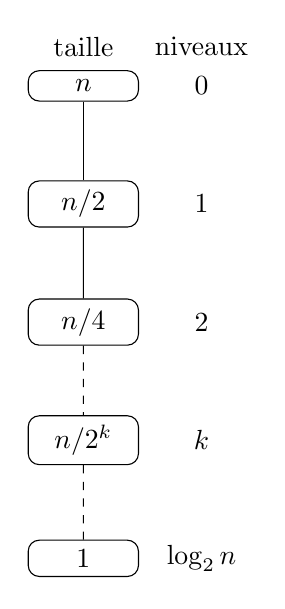
\begin{tikzpicture}[invis/.style={draw=none}]
    \tikzstyle{level 1}=[edge from parent/.style={draw}, sibling distance=17mm]
    \tikzstyle{level 3}=[edge from parent/.style={draw,dashed}, sibling distance=17mm]
    \tikzstyle{level 5}=[edge from parent/.style={draw=none}, sibling distance=17mm]
    \tikzstyle{level 10}=[edge from parent/.style={draw=none}, level distance=5mm]
    \tikzstyle{level 11}=[edge from parent/.style={draw=none}, level distance=15mm]
    \tikzstyle{every node}=[fill=white,rectangle, rounded corners,draw=black,solid,minimum width=14mm]
    \tikzstyle{every node}=[fill=white,rectangle, rounded corners,draw=black,solid,minimum width=14mm]
    \node {$n$}
    child {node {$n/2$}
      child {node {$n/4$}
        child {node {$n/2^k$}
          child {node {$1$}
            child[grow=right] {node[invis] {$\log_2 n$}
              child[grow=up] {node[invis] {$k$}
                child[grow=up] {node[invis] {2}
                  child[grow=up] {node[invis] {1}
                    child[grow=up] {node[invis] {0}
                      child[grow=up] {node[invis] {niveaux}
                        child[grow=left] {node[invis] {taille}
                        }
                      }
                  }
                }
              }
            }
          }
        }
      }
    }
};
  \end{tikzpicture}
\end{minipage}
\hfill\begin{minipage}[r]{.6\linewidth}
  \only<2->{Niveau $k$}
  \begin{itemize}
  \item<2-> $\mathbf{1}$ sous problème de taille $\mathbf{n/2^k}$
  \item<2-> $\Theta(1)$ opérations élémentaires  par niveau
  \end{itemize}
  \only<3->{Total:}
  \begin{itemize}
  \item<3-> taille du problème divisée par 2 à chaque niveau $\implies \log_2 n +1$ niveaux.
  \item<4-> \underline{Complexité} = $\Theta(\log n)$
\end{itemize}
\end{minipage}
\end{frame}
\begin{frame}{Diviser pour régner : Multiplication d'entiers}
  \begin{tabbing}
  \underline{Entrées} \= $x,y$ entiers de $\mathbf{n}$ chiffres en base $r$ \\
  \underline{Sortie}  \>  $x*y$
\end{tabbing}
\end{frame}


%%=======================================
%%=======================================
%\lecture{Représentation des entiers}{lec-binaire}
%%=======================================
%%=======================================

\begin{frame}{Représentation des entiers positifs}
La représentation numérique d'un entier poitif $x$ de $n$ chiffres en \red{\textbf{base $\mathbf{b}$}} est la suite 
$(x_{n-1}, x_{n-2} \ldots x_{0})$ des entiers $x_i \in [0,\ldots b)$, tels que ~\\~\\

$x=x_{n-1}b^{n-1}+x_{n-2}b^{n-2} \ldots + x_{2}b^{2}+x_{1}b+ x_{0} = \sum_{i=0}^{n-1} x_{i}b^{i} $

~\\~\\
\uncover<2->{En base {\red{$\mathbf{b}$}}, avec \red{$\mathbf{k}$} chiffres \\
  \begin{itemize}
  \item<3->[] $\red{\mathbf{\rightarrow}}$ représenter les entiers $\mathbf{0},\ldots,\mathbf{b^k-1}$
  \item<4->[] ex: $b = 10, k=4$ : entiers entre $0$ et $9999 = 10^4 -1$ 
  \end{itemize}}
\uncover<5->{Ainsi, la taille de \textbf{x} en base \textbf{b} est $\red{\mathbf{\lceil\log_b(x+1)\rceil}}$}

\end{frame}

\begin{frame}{Représentation binaire des entiers positifs}
Représentation binaire des entiers positifs (b=2) un exemple
~\\~\\
$
  \begin{array}{|*{8}{c|}}
    \hline
    1 & 0 & 0 & 1 & 1 & 0 & 1 & 1 \\
    \hline
  \end{array}
  =$ \only<1>{\mbox{???}}\only<2->{~\\~\\ $1 \times 2^7 + 0 \times 2^6 + 0  \times 2^5 + 1 \times 2^4 + 1 \times 2^3 + 0 \times 2^2 + 1 \times
  2^1 + 1 \times 2^0 $}
\only<3->{~\\ $= 128 + 0 +0 + 16 + 8 + 0 + 2 + 1$}
\only<4->{~\\ $=  155$}

%\textbf{Nombre de bits} nécessaires pour représenter un entier $\mathbf{n}$ ?
%~\\~\\
%\uncover<2->{En base {\red{$\mathbf{b}$}}, avec \red{$\mathbf{k}$} chiffres \\
%  \begin{itemize}
%  \item<3->[] $\red{\mathbf{\rightarrow}}$ représenter les entiers $\mathbf{0},\ldots,\mathbf{b^k-1}$
%  \item<4->[] ex: $b = 10, k=4$ : entiers entre $0$ et $9999 = 10^4 -1$ 
%  \end{itemize}}
%\uncover<5->{Ainsi, la taille de \textbf{x} en base \textbf{b} est $\red{\mathbf{\lceil\log_b(x+1)\rceil}}$}
~\\~\\
\uncover<6->{\textbf{nombre de bits} pour représenter l'entier \textbf{x}  $\red{\mathbf{\lceil\log_2(x+1)\rceil}} = \red{\mathbf{\Theta(\log(x))}}$}

\end{frame}


\begin{frame}{Diviser pour régner : Multiplication d'entiers}
  \begin{tabbing}
  \underline{Entrées} \= $x,y$ entiers de $\mathbf{n}$ chiffres en base $r$ \\
  \underline{Sortie}  \>  $x*y$
\end{tabbing}

\underline{Karatsuba}
\begin{tabbing}
  $x  = $ \framebox[3\width]{$x_L$} \framebox[3\width]{$x_R$} $ = x_L\cdot{}r^{n/2} + x_R$ \\
  $y  = $ \framebox[3\width]{$y_L$} \framebox[3\width]{$y_R$} $ = y_L\cdot{}r^{n/2} + y_R$ \\
\end{tabbing}

\only<2-3>{$xy = x_Ly_L\cdot{}r^n + (x_Ly_R + y_Lx_R)\cdot{}r^{n/2} + x_Ry_R$}\only<4>{$xy = $\framebox{\red{$\mathbf{x_Ly_L}$}}$\cdot{}r^n + (x_Ly_R + y_Lx_R)\cdot{}r^{n/2} + $\framebox{\red{$\mathbf{x_Ry_R}$}}} ~\\
\only<3>{$x_Ly_R + y_Lx_R = (x_L+x_R)(y_L+y_R)-x_Ly_L - x_Ry_R$}\only<4>{$x_Ly_R + y_Lx_R = $\framebox{\red{$\mathbf{(x_L+x_R)(y_L+y_R)}$}} $-x_Ly_L - x_Ry_R$} ~\\~\\

\uncover<4->{\red{\textbf{3 multiplications}} d'entiers de \red{$\mathbf{n/2}$} chiffres}
\end{frame}


\begin{frame}{Diviser pour régner}
  \begin{enumerate}
  \item<1-> \underline{Problème} : multiplier \\
  $x  = $ \framebox[3\width]{$x_L$} \framebox[3\width]{$x_R$} \hfill $\mathbf{n}$ chiffres \\
  $y  = $ \framebox[3\width]{$y_L$} \framebox[3\width]{$y_R$} \hfill $\mathbf{n}$ chiffres \\
  \item<2-> \underline{Sous problèmes} : multiplier des entiers de $\mathbf{\frac{n}{2}}$ (+1) chiffres
    \noindent\begin{tabular}[l]{ccc}
    $x_L$ & $~x_R$ & $~x_L+x_R$ \\
      $y_L$& $~y_R$ & $~y_L+y_R$ 
    \end{tabular}
    \item<3-> \underline{Combiner} les solutions des sous problèmes\\
      $xy = x_Ly_Lr^n + ((x_L+x_R)(y_L+y_R)-x_Ly_L - x_Ry_R)r^{n/2} + x_Ry_R$ \\
      \uncover<4->{$\mathbf{\red{\rightarrow}}$ complexité $O(n)$}
  \end{enumerate}
\end{frame}

\begin{frame}{Algorithme ``diviser pour régner'' pour la multiplication}
  \begin{tabbing}
    aaa\=aaa\=aaa\=\kill
    \textbf{\red{Multiplier}}($x,y$) \texttt{/* x,y entiers positifs en base r */} \\
    \> entier $n,p_1,p_2,p_3$ \\
    \> $n \leftarrow \max($taille de $x$, taille de $y)$ \\
    \> \textbf{si} $n = 1$ \textbf{alors} \textsl{retourner} $xy$ \textbf{fin si}\\
    \> $x_L \leftarrow$ $\lfloor  \frac{n}{2} \rfloor$ premiers chiffres de $x$;
     $x_R \leftarrow$ $\lceil \frac{n}{2} \rceil$ derniers chiffres  de $x$ \\ 
    \> $y_L \leftarrow$ $\lfloor \frac{n}{2} \rfloor$ premiers chiffres de $y$;
     $y_R \leftarrow$ $\lceil \frac{n}{2} \rceil$ derniers chiffres de $y$  \\
    \> $p_1 \leftarrow $ \textbf{\red{Multiplier}}($x_L,y_L$) \\
    \> $p_2 \leftarrow $ \textbf{\red{Multiplier}}($x_R,y_R$) \\*
    \> $p_3 \leftarrow $ \textbf{\red{Multiplier}}($x_L+x_R,y_L+y_R$) \\
    \> \textsl{retourner} $p_1 \times r^n + (p_3 - p_2 - p_1) \times r^{n/2} + p_2$
  \end{tabbing}
  
\end{frame}


\begin{frame}{Analyse}
  \only<1->{
    \begin{tabbing}
    aaa\=aaaaaaaaaaaaaaaaaaaaaaaaaaaaaaaaaaaaaaaaaaaaaaaa\=\kill
    \textbf{Multiplier}($x,y$) \texttt{/* x,y entiers positifs en base r */} \\
    \> $n \leftarrow \max($taille de $x$, taille de $y)$ \\
    \> \textbf{si} $n = 1$ \textbf{alors} \textsl{retourner} $xy$ \textbf{fin si}\\
    \> $x_L \leftarrow$ $\lfloor  \frac{n}{2} \rfloor$ premiers chiffres de $x$;
     $x_R \leftarrow$ $\lceil \frac{n}{2} \rceil$ derniers chiffres  de $x$ \\ 
    \> $y_L \leftarrow$ $\lfloor \frac{n}{2} \rfloor$ premiers chiffres de $y$;
     $y_R \leftarrow$ $\lceil \frac{n}{2} \rceil$ derniers chiffres de $y$  \\
       \> $p_1 \leftarrow $ \textbf{Multiplier}($x_L,y_L$) \only<3->{\> $\red{\mathbf{T(n/2)}}$} \\
    \> $p_2 \leftarrow $ \textbf{Multiplier}($x_R,y_R$) \only<3->{\> $\red{\mathbf{T(n/2)}}$} \\
    \> $p_3 \leftarrow $ \textbf{Multiplier}($x_L+x_R,y_L+y_R$) \only<3->{\> $\red{\mathbf{T(n/2)}}$} \\
    \> \textsl{retourner} $p_1 \times r^n + (p_3 - p_2 - p_1) \times r^{n/2} + p_2$ \only<3->{\> $\red{\mathbf{O(n)}}$} 
  \end{tabbing}
}
Supposons $n = 2^k$, $k$  entier $\geq 0$ \\
\only<2>{
  T(n) = ???
}\only<3->{
$\red{\mathbf{T(n)} = \mathbf{3T(n/2) + cn}}$}
\end{frame}

\begin{frame}{Arbre récursif}
\begin{tikzpicture}[skip/.style={edge from parent/.style={dashed,draw,black}},
  norm/.style={edge from parent/.style={solid,black,draw}},
  invis/.style={draw=none}]
    \tikzstyle{every node}=[fill=white,rounded corners,draw=black,solid]
    \tikzstyle{level 1}=[sibling distance=32mm]
    \tikzstyle{level 2}=[sibling distance=10mm]
    \tikzstyle{level 3}=[sibling distance=4mm,level distance=20mm]
    \tikzstyle{level 4}=[sibling distance=4mm,level distance=10mm]
    \tikzstyle{level 5}=[level distance=10mm,edge from parent/.style={draw=none}]
    \tikzstyle{level 6}=[level distance=15mm,edge from parent/.style={draw=none}]
    \tikzstyle{level 10}=[level distance=6mm]
    \node {taille $\mathbf{n}$}
    child { node {taille $\mathbf{n/2}$}
      child { node {$\mathbf{n/4}$} 
        child[skip] { node {$\mathbf{2}$} 
          child[norm] {node {$\mathbf{1}$}} 
          child[norm] {node {$\mathbf{1}$}}
          child[norm] {node {$\mathbf{1}$}}
        }
        child[skip]
        child[skip]
      }
      child {node {$\mathbf{n/4}$}}
      child {node {$\mathbf{n/4}$}}
    }
      child {node {taille $\mathbf{n/2}$}
        child {node {$\mathbf{n/4}$}}
        child {node {$\mathbf{n/4}$}}
        child {node {$\mathbf{n/4}$}}
      } 
      child {node {taille $\mathbf{n/2}$}
        child {node {$\mathbf{n/4}$}}
        child {node {$\mathbf{n/4}$}}
        child {node {$\mathbf{n/4}$}
          child[skip]
          child[skip]
          child[skip] { node {$\mathbf{2}$} 
            child[norm] {node {$\mathbf{1}$}} 
            child[norm] {node {$\mathbf{1}$}}
            child[norm] {node {$\mathbf{1}$}
              child[grow=right] {node[invis] {\only<4->{$\red{\mathbf{\log{}n}}$}}
                child[grow=up] {
                  child[grow=up] {node[invis] {\only<3->{$\red{\mathbf{2}}$} }
                    child[grow=up] {node[invis] {\only<3->{$\red{\mathbf{1}}$}}
                      child[grow=up] {node[invis] {\only<2->{$\red{\mathbf{0}}$}}
                        child[grow=up] {node[invis] {\red{niveaux}}
                        }
                      }
                    }
                  }
                }
              }
            }
          }
      }
    };
  \end{tikzpicture}
\end{frame}

\begin{frame}{Complexité}
  \begin{tikzpicture}[invis/.style={draw=none}]
    \tikzstyle{level 1}=[edge from parent/.style={draw=none}, sibling distance=17mm]
    \tikzstyle{level 2}=[edge from parent/.style={draw}]
    \tikzstyle{every node}=[fill=white,rounded corners,draw=black,solid]
    \node[invis] {\large\red{\textbf{Niveau} $\mathbf{k}$}}
    child {node {$\only<1>{\mathbf{n/???}}\only<2->{\mathbf{n/2^k}}$}
      child {node {$\only<1>{\mathbf{n/???}}\only<2->{\mathbf{n/2^{k+1}}}$}}
      child {node {$\only<1>{\mathbf{n/???}}\only<2->{\mathbf{n/2^{k+1}}}$}}
      child {node {$\only<1>{\mathbf{n/???}}\only<2->{\mathbf{n/2^{k+1}}}$}}
    }
    child {node {$\only<1>{\mathbf{n/???}}\only<2->{\mathbf{n/2^k}}$}
      % child {node {$\only<3->{\mathbf{n/2^{k+1}}}$}}
      % child {node {$\only<3->{\mathbf{n/2^{k+1}}}$}}
      % child {node {$\only<3->{\mathbf{n/2^{k+1}}}$}}
    }
    child {node[invis] {$\ldots$} edge from parent[draw=none]}
    child {node[invis] {$\ldots$} edge from parent[draw=none]}
    child {node {$\only<1>{\mathbf{n/???}}\only<2->{\mathbf{n/2^k}}$}
      child {node {$\only<1>{\mathbf{n/???}}\only<2->{\mathbf{n/2^{k+1}}}$}}
      child {node {$\only<1>{\mathbf{n/???}}\only<2->{\mathbf{n/2^{k+1}}}$}}
      child {node {$\only<1>{\mathbf{n/???}}\only<2->{\mathbf{n/2^{k+1}}}$}}
    }
    ;
  \end{tikzpicture}
  \begin{itemize}
  \item<3-> $\red{\mathbf{3^k}}$ sous problèmes, chacun de taille $\red{\mathbf{n/2^{k}}}$
  \item<4-> résolution \emph{d'un problème} de taille $\red{\mathbf{n/2^k}}$ : combiner les solutions de 3 sous problèmes $\longrightarrow \red{\mathbf{O(n/2^k)}}$ opérations
  \item<5->[$\red{\mathbf{\implies}}$] $\red{3^k \times \mathbf{O(n/2^k)}} = (3/2)^k \times O(n)$ opérations au niveau $\red{\mathbf{k}}$ de récursion
  \end{itemize}
\end{frame}

\begin{frame}{Complexité}
  \begin{center}
    {\large\textbf{\red{total}}}
  \end{center}
  \begin{itemize}
  \item<1-> Niveau $k$ :  $\red{\mathbf{(3/2)^k \times O(n)}}$ opérations
  \item<2-> La taille des sous problèmes est divisée par 2 à chaque niveau $\red{\implies \mathbf{O(\log_2(n))}}$ niveaux
  \item<3-> \underline{Au total}:
  \end{itemize}
  \only<3->{
    $$
    \sum_{k=0}^{\log_2(n)} \left(\frac{3}{2}\right)^k \times O(n) = O\left(n\frac{3^{\log_2 n}}{2^{\log_2 n}}\right) = \mathbf{O(3^{\log_2 n})} =$$ $$\red{\mathbf{O(n^{\log_2 3})}}\simeq O(n^{1,59})
    $$
  }
\end{frame}


\begin{frame}{Analyse des algorithmes diviser pour régner}
  \begin{theorem}[Théorème général] 
Soient $a \geq 1$ et $b>1$  deux constantes, soit $f(n)$ une fonction et soit $T(n)$ définie pour les entiers non négatifs par la récurrence $T(n) = aT(n/b) + f(n)$ où l'on interprète $n/b$ comme signifiant $\lceil n/b \rceil$ ou $\lfloor n/b \rfloor$, $T(n)$ peut être bornée de la façon suivante  :  

\begin{enumerate}
  \item Si $f(n)=O(n^{log_b(a)-\epsilon})$ pour une certaine constante $\epsilon >0$  alors $T(n)=\Theta(n^{log_b(a)})$ \\
   \item Si $f(n)=\Theta(n^{log_b(a)})$  alors $T(n)=\Theta(n^{log_b(a)}logn)$ \\
   \item Si $f(n)=\Omega(n^{log_b(a)+\epsilon})$ pour une certaine constante $\epsilon > 0$ et si   $a f(n/b)\leq cf(n)$ pour une constante $c<1$ et pour n suffisamment grand alors $T(n)=\Theta(f(n))$
  \end{enumerate}  
\end{theorem}
\end{frame}


%============================================
%============================================
\lecture{Structures de données élémentaires}{lec-sdelem}
%============================================
%============================================
% \begin{frame}
%   \begin{center}
%     \Large{\red{Structures de données }}
%   \end{center}
% \end{frame}


\begin{frame}{Objectifs}
  Gérer un \emph{ensemble} d'éléments (données)
  \begin{itemize}
  \item dynamique: données ajoutées/supprimées au cours du temps
  \item éléments de types variés: entiers, chaînes de caractères,
    objets complexes, etc.
  \end{itemize}
  \red{\textbf{Opérations}} sur les données:
  \begin{itemize}
  \item \textbf{Tester} si l'ensemble est \textbf{vide}
  \item \textbf{Insertion}/\textbf{suppression}
  \item \textbf{Chercher} un élément
  \item Éventuellement requêtes plus sophistiquées
  \end{itemize}
\end{frame}


\begin{frame}{Type de données abstrait et Structures de données}
\begin{itemize}
  \item Un \emph{type de données abstrait} est la description d’un ensemble organisé d’objets et des opérations qui les manipulent. 
\item Une \emph{structure de données} est l’implémentation explicite d’un type de données : 
\begin{itemize}
\item expliciter comment les objets sont représentés en termes de types élémentaires et d’autres types abstraits 
\item donner les algorithmes qui implementent les opérations.
 \end{itemize}
  \end{itemize}
Lorsqu’un type de données est implémenté, on peut l'utiliser dans l’implémentation de types de données plus complexes. Ceci conduit à une hïerarchie de types, où l’on trouve, tout en bas de l’échelle, des types  élémentaires comme les booléens, entiers, réels, tableaux etc.
  \end{frame}

\begin{frame}{Pile -- spécification}
Une pile est une suite finie d'éléments où les suppressions mettent en {\oe}uvre le principe \textbf{dernier entré, premier sorti} (\emph{LIFO}: \emph{last in, first out}).

  \red{Opérations :}
  \begin{itemize}
  \item $P \leftarrow \mathbf{CreerPileVide()}$
  \item $\mathbf{EstVide}(P)$ \\
    \emph{retourne \textbf{vrai} si la pile est vide, \textbf{faux} sinon}
  \item $\mathbf{Empiler}(P,e)$ \\
    \emph{insère $e$ au \textbf{sommet} de la pile, retourne rien}
  \item $\mathbf{Depiler}(P)$ \\
    \emph{retourne l'élément au \textbf{sommet}  et le
      supprime de la pile}
  \item $\mathbf{Sommet}(P)$ \\
    \emph{retourne l'élément au \textbf{sommet}  \underline{sans} le
      supprimer de la pile}
  \end{itemize}
\end{frame}



\begin{frame}{Pile -- exemple}
  \begin{minipage}{.3\linewidth}
    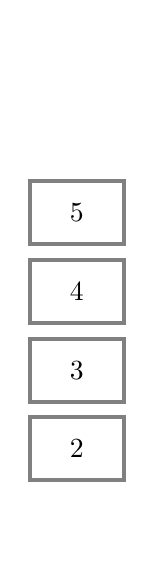
\begin{tikzpicture}[invis/.style={draw=none, minimum width=1.2cm, minimum height=.7cm, line width=1.4pt},
      cell/.style={draw=gray,minimum width=1.2cm, minimum height=.8cm, line width=1.4pt}]
      \foreach \d in {1,...,7} {
        \path   node[invis](R_\d)  at (0,\d) {\phantom{10}};
      }
      \foreach \d in {2,...,3} {
        \node[cell,visible on = <\d->]   at (R_\d) {\d};
      }
      \node[cell,visible on = <4-6>]   at (R_4) {4};
      \node[cell,visible on = <5-5>]   at (R_5) {5};
    \end{tikzpicture}
  \end{minipage}
  \begin{minipage}{.6\linewidth}
    \uncover<1->{$P \leftarrow$ \textbf{CreerPileVide}()} \\
    \uncover<2->{\textbf{Empiler}($P,2$)} \\
    \uncover<3->{\textbf{Empiler}($P,3$)} \\
    \uncover<4->{\textbf{Empiler}($P,4$)} \\
    \uncover<5->{\textbf{Empiler}($P,5$)} \\
    \uncover<6->{$x \leftarrow $ \textbf{Dépiler}($P$) \hfill \texttt{/* x = 5 */}}\\
    \uncover<7->{$x \leftarrow x+$ \textbf{Dépiler}($P$) \hfill \texttt{/* x = 9 */}}\\
    % \begin{tabbing}
    %   aaa\=aaaaa\=\kill
    %   \>  \\
    %   \> \uncover<2->{
    %   \> \uncover<3->{\textbf{Empiler}($P,4$)} \\
    %   \> \uncover<4->{\textbf{Empiler}($P,8$)} \\
    %   \> \uncover<5->{$x \leftarrow$ \textbf{Dépiler}($P$) \> \texttt{/* x = 2   */}}\\
    %   \> \uncover<6->{\textbf{Empiler}($F,7$); \textbf{Empiler}($P,5$); \textbf{Empiler}($F,3$);} \\
    %   \> \uncover<9->{$x \leftarrow x + $\textbf{Dépiler}($P$)} \\
    %   \> \uncover<10>{$x \leftarrow x + $\textbf{Dépiler}($P$); \> \texttt{/* x = 14 */}}
    % \end{tabbing}
 \end{minipage}
\end{frame}



\begin{frame}{Pile -- utilisation}
  \begin{itemize}
  \item gestion des appels de fonctions
  \item pages visités par un navigateur web
  \item annulation des modification d'un document (undo)
  \item évaluation d'expressions arithmétiques
  \item ...
  \end{itemize}
\end{frame}

\begin{frame}{Expressions arithmétiques}
  Une expression arithmétique se compose (version simplifiée)
  \begin{itemize}
  \item d'entiers naturels (i.e., $\geq 0$)
  \item d'opérateurs $+,*$ 
  \end{itemize}

  \uncover<2->{
    Une expression \red{\textbf{postfixée}} est :
    \begin{itemize}
    \item<3-> un entier naturel
    \end{itemize}
    ou de la forme
    \begin{itemize}
    \item<4-> $\mathbf{~~e1~~ e2~~ +}$ 
    \item<4-> $\mathbf{~~e1~~ e2~~ *}$
  \end{itemize}
 \uncover<4>{où $\mathbf{e1,e2}$ sont des expressions postfixées}}
\end{frame}

\begin{frame}{Expressions postfixées}
  \begin{tabular}{>{\ttfamily}l|l}
    \multicolumn{1}{l|}{Expression} & Évaluation \\
    \hline 
    21 & \uncover<2->{21} \\
    2 3 * & \uncover<3->{6} \\
    12 8 + & \uncover<4->{20} \\
    2 3 * 12 8 + + & \uncover<5->{26} \\
    30 32 +  6 8 + * 2 3 * 95 96 + * + & \uncover<6->{2014} 
  \end{tabular}
~\\~\\~\\
\uncover<7>{\underline{Représentation} : tableau \\
  \begin{tabbing}
    aaa\=aaa\=\kill
  \> \texttt{30 32 +  6 8 + * 2 3 * 95 96 + * +} \\
  \>
  \begin{tabular}{|*{15}{>{\ttfamily}l|}}
    \hline 
    30 &  32 & + &  6 & 8 & + & * & 2 & 3 & * & 95 & 96 & + & * & + \\
    \hline
  \end{tabular}
  \end{tabbing}
}
\end{frame}

\begin{frame}{Évaluation d'expressions postfixées}
  \begin{itemize}
  \item[\underline{entrée} :] tableau \textbf{T} représentant une expression postfixée \red{e}, \\sa taille \textbf{n}
  \item[\underline{sortie} :] l'évaluation de l'expression \red{e}
  \end{itemize}
~\\
  \uncover<2->{On dispose
    \begin{itemize}
    \item d'une \red{\textbf{pile}}
    \item d'une fonction \red{\textbf{calcul}} d'évaluation d'expr. élémentaires 
    \end{itemize}

    \begin{tabbing}
      aaa\=aaa\=\kill
      \textbf{calcul}(op,a,b) \hfill \texttt{/* op: opérateur + ou *; a,b: entiers */} \\
      \> \textbf{si} op $=$ \texttt{'+'} \textbf{alors} retourner $a+b$ \textbf{fin si} \\
      \> \textbf{si} op $=$ \texttt{'*'} \textbf{alors} retourner $a*b~$ \textbf{fin si} \\
    \end{tabbing}
}
\end{frame}

\begin{frame}{Évaluation d'expressions postfixées}
  \underline{principe }:
  \begin{itemize}
  \item<1-> Parcourir le tableau
  \item<2-> Empiler les entiers rencontrés
  \item<3-> Lorsqu'un opérateur \red{\texttt{op}} est rencontré:
    \uncover<4->{\begin{itemize}
      \item Dépiler les deux derniers entiers \red{\texttt{a}} et \red{\texttt{b}}
      \item Calculer \red{\texttt{a op b}}
      \item Empiler le résultat 
      \end{itemize}}
  \end{itemize}
\end{frame}

\begin{frame}{Évaluation d'expressions postfixées : exemple}
  \red{entrée :}
    \begin{tabular}{|*{15}{>{\ttfamily}l|}}
      \hline 
      30 &  32 & + &  6 & 8 & + & * & 2 & 3 & * & 95 & 96 & + & * & + \\
      \hline
    \end{tabular}

Évolution de la pile \\
\uncover<1->{\begin{tabular}{|C{.9cm}|}
  \\
  \\
  \hline
  30 \\
  \hline
\end{tabular}}
\uncover<2->{\begin{tabular}{|C{.9cm}|}
  \\
  \hline
  32 \\
  \hline
  30 \\
  \hline
\end{tabular}}
\uncover<3->{\begin{tabular}{|C{.9cm}|}
  \\
  \\
  \hline
  \red{62} \\
  \hline
\end{tabular}}
\uncover<4->{\begin{tabular}{|C{.9cm}|}
  \\
  \hline
  6 \\
  \hline
  62\\
  \hline
\end{tabular}}
\uncover<5->{\begin{tabular}{|C{.9cm}|}
  \hline
  8 \\
  \hline
  6 \\
  \hline
  62\\
  \hline
\end{tabular}}
\uncover<6->{\begin{tabular}{|C{.9cm}|}
   \\
  \hline
  \red{14} \\
  \hline
  62\\
  \hline
\end{tabular}}
\uncover<7->{\begin{tabular}{|C{.9cm}|}
     \\ \\
  \hline
  \red{868} \\
  \hline
\end{tabular}}
\uncover<8->{\begin{tabular}{|C{.9cm}|}
    \\ \\
  \hline
  2 \\
  \hline
  868 \\
  \hline
\end{tabular}}
\uncover<9->{\begin{tabular}{|C{1cm}|}
  \\
  \hline
  3 \\
  \hline
  2 \\
  \hline
  868 \\
  \hline
\end{tabular}}
\uncover<10->{\begin{tabular}{|C{.9cm}|}
  \\ \\
  \hline
  \red{6} \\
  \hline
  868 \\
  \hline
\end{tabular}}
\uncover<11->{\begin{tabular}{|C{.9cm}|}
  \\
  \hline
  95 \\
  \hline
  6 \\
  \hline
  868 \\
  \hline
\end{tabular}}
\uncover<12->{\begin{tabular}{|C{.9cm}|}
  \hline
  96 \\
  \hline
  95 \\
  \hline
  6 \\
  \hline
  868 \\
  \hline
\end{tabular}}
\uncover<13->{\begin{tabular}{|C{.9cm}|}
  \\
  \hline
  \red{191} \\
  \hline
  6 \\
  \hline
  868 \\
  \hline
\end{tabular}}
\uncover<14->{\begin{tabular}{|C{.9cm}|}
  \\ \\
  \hline
  \red{1146} \\
  \hline
  868 \\
  \hline
\end{tabular}}
\uncover<15->{\begin{tabular}{|C{.9cm}|}
  \\ \\
  \hline
  \red{2014} \\
  \hline
\end{tabular}}


\end{frame}

\begin{frame}{Évaluation d'expressions postfixées : algorithme}
  \begin{tabbing}
    aaa\=aaa\=aaa\=\kill
    \red{EvalExprPostfixée}(\textbf{T},\textbf{n}) \texttt{/* T: tableau représentant } \\
    \> \>   \texttt{une expr. postfixée, n: taille de T */} \\
    \> $P \leftarrow$ \textbf{CreerPileVide}() \\
    \> entier $a,b$ \\
    \> \textbf{pour} $i$  \textbf{allant de} $1$ \textbf{à} $n$ \textbf{faire} \\
    \> \> \textbf{si} \emph{estNombre($T[i]$)} \textbf{alors} \textbf{empiler}($P,T[i]$) \textbf{fin si} \\
    \> \> \textbf{si} \emph{estOpérateur($T[i]$)} \textbf{alors} \\
    \> \> \> $a \leftarrow $\textbf{dépiler}($P$) \\
    \> \> \> $b \leftarrow $\textbf{dépiler}($P$) \\
    \> \> \> \textbf{empiler}($P$, \textbf{calcul}($T[i]$,$a$,$b$)) \\
    \> \> \textbf{fin si} \\
    \> \textbf{fin pour}\\
    \> \textsl{retourner} \textbf{dépiler}($P$)
  \end{tabbing}
\end{frame}

\begin{frame}{Pile -- mise en {\oe}uvre}
  Ingrédients:
  \begin{itemize}
  \item<1-> Tableau \textbf{T} de taille $\mathbf{N}$
  \item<2-> Variable \textbf{hauteur}, initialement $0$
  \item<3-> $\mathbf{N}$ : nombre maximal d'éléments dans la pile
  \end{itemize}
  
  %\uncover<4>{Attention : ici indices du tableau sont $1,\ldots,\mathbf{N}$}
\end{frame}

\begin{frame}{Pile -- mise en {\oe}uvre}

\begin{tabbing}
  aaa\=aaa\=\kill
  \red{Empiler}($x$) \\
  \uncover<2->{
    \>  \textbf{si} $hauteur = N$ \textbf{alors} \textsl{afficher} \texttt{erreur:pile pleine} \\
    \>  \textbf{sinon} $hauteur \leftarrow hauteur + 1$; $T[hauteur] \leftarrow x$;  \\
    \>  \textbf{fin si}}
  \end{tabbing}

~\\

\begin{tabbing}
  aaa\=aaa\=\kill
  \red{Dépiler}() \\
  \uncover<3->{
    \> \textbf{si} $hauteur = 0$ \textbf{alors} \textsl{afficher} \texttt{erreur:pile vide} \\
    \> \textbf{sinon} $hauteur \leftarrow hauteur - 1$; \textsl{retourner} $T[hauteur+1]$ \\
    \> \textbf{fin si}}
\end{tabbing}

~\\
\begin{tabbing}
  aaa\=aaa\=\kill
  \red{EstVide}() \\
  \uncover<4->{
    \> \textsl{retourner} $hauteur = 0$}
  \end{tabbing}
~\\

\uncover<5->{Complexité : \textbf{O(1)}}
\end{frame}


\begin{frame}{File -- spécification}
Une file est une suite finie d'éléments où les suppressions mettent en {\oe}uvre le principe \textbf{premier entré, premier sorti} (\emph{FIFO}: \emph{first in, first out}).\\
La file comporte une \emph{tête} et une \emph{queue}. Lorsqu’un élément est inséré, il prend place à la  \emph{queue} de la file. L’élément supprimé est toujours le premier en  \emph{tête} de la file.

  \red{Opérations :}
  \begin{itemize}
  \item $F \leftarrow \mathbf{CreerFileVide()}$
  \item $\mathbf{EstVide}(F)$ \\
    \emph{retourne \textbf{vrai} si la file est vide, \textbf{faux} sinon}
  \item $\mathbf{Enfiler}(F,e)$ \\
    \emph{insère $e$ en \textbf{queue} de la file}
  \item $\mathbf{Defiler}(F)$ \\
    \emph{retourne l'élément de \textbf{tête}  et le
      supprime de la file}
  \end{itemize}
%\uncover<2->{Ordre \emph{FIFO}: first in, first out}
\end{frame}

\begin{frame}{File -- exemple}
  
\begin{tikzpicture}[invis/.style={draw=none, minimum width=1cm, minimum height=.8cm, line width=1.4pt}]
    \foreach \d in {-2,-1,...,7} {
      \path   node[invis](R_\d)  at (\d,0) {\phantom{10}};
    }
    \path (R_1) ++(110:.6cm) node[draw=none] (deb) {};
    \path (R_5) ++(70:.6cm) node[draw=none] (fin) {};
    \draw[draw=blue,->,very thick,visible on=<1->] (deb)  -- (fin);
    \node[draw=none,visible on=<2-4>] at (R_5) {\textbf{2}};
    \node[draw=none,visible on=<3-4>] at (R_4) {\textbf{4}};
    \node[draw=none,visible on=<4-4>] at (R_3) {\textbf{8}};
    \node[draw=none,visible on=<5-8>] at (R_5) {\textbf{4}};
    \node[draw=none,visible on=<5-8>] at (R_4) {\textbf{8}};
    \node[draw=none,visible on=<6-8>] at (R_3) {\textbf{7}};
    \node[draw=none,visible on=<7-8>] at (R_2) {\textbf{5}};
    \node[draw=none,visible on=<8-8>] at (R_1) {\textbf{3}};
    \node[draw=none,visible on=<9>] at (R_5) {\textbf{8}};
    \node[draw=none,visible on=<9>] at (R_4) {\textbf{7}};
    \node[draw=none,visible on=<9>] at (R_3) {\textbf{5}};
    \node[draw=none,visible on=<9>] at (R_2) {\textbf{3}};
    \node[draw=none,visible on=<10>] at (R_5) {\textbf{7}};
    \node[draw=none,visible on=<10>] at (R_4) {\textbf{5}};
    \node[draw=none,visible on=<10>] at (R_3) {\textbf{3}};

    
\end{tikzpicture}
~\\~\\
\begin{tabbing}
 aaa\=aaaaaaaaaaaaaaaaaaaaaaaaaaaaaaaaaaaaaaaaaaa\=\kill
 \> \uncover<1->{$F \leftarrow$ \textbf{CreerFileVide}()} \\
 \> \uncover<2->{\textbf{Enfiler}($F,2$)} \\
 \> \uncover<3->{\textbf{Enfiler}($F,4$)} \\
 \> \uncover<4->{\textbf{Enfiler}($F,8$)} \\
 \> \uncover<5->{$x \leftarrow$ \textbf{Défiler}($F$) \> \texttt{/* x = 2   */}}\\
 \> \uncover<6->{\textbf{Enfiler}($F,7$); \textbf{Enfiler}($F,5$); \textbf{Enfiler}($F,3$);} \\
 \> \uncover<9->{$x \leftarrow x + $\textbf{Défiler}($F$) \> \texttt{/* x = 6   */}}\\
 \> \uncover<10>{$x \leftarrow x + $\textbf{Défiler}($F$); \> \texttt{/* x = 14 */}}
\end{tabbing}
\end{frame}


\begin{frame}{File: mise en {\oe}uvre à l’aide d'un tableau}
Ingrédients:
  \begin{itemize}
  \item \textbf{T} : Tableau de taille \textbf{N}
  \item \textbf{deb} : indice dans le tableau du premier élément de la file
  \item \textbf{lg} : longueur de la file
  \item (au plus \textbf{N} éléments dans la file)
  \end{itemize}  
\end{frame}


 \begin{frame}{Tampon circulaire}
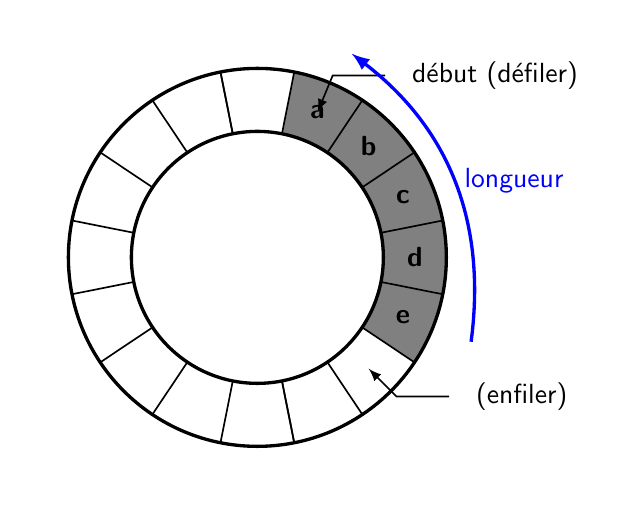
\begin{tikzpicture}[>=latex,font=\sffamily,semithick,scale=2]
  \foreach \id / \angle in
  {0/0,1/22.5,2/45,3/67.5,4/90,5/112.5,6/135,7/157.5,8/180,9/202.5,10/225,11/247.5,
    12/270,13/292.5,14/315,15/337.5}{
    \node(C\id) at (\angle:1) {}; 
    \node(O\id) at (\angle:1.4) {}; 
    \node(I\id) at (\angle:.8) {}; 
  }
  \fill [gray] (0,0) -- (78.75:1.2) arc [end angle=-33.75, start angle=78.75, radius=1.2] -- cycle;
  \foreach \angle in {101.25,78.75,...,-78.75}
  \draw (\angle:1.2) -- (\angle-180:1.2);
  \draw [black,very thick] (0,0) circle (1.2);

  \draw [<-] (67.5:1) -- (67.5:1.25) -- +(.333,0)
  node [right,inner xsep=.333cm] (Head) {\red{début} (défiler)};
  \draw [<-] (-45:1) -- (-45:1.25) -- +(.333,0)
  node [right,inner xsep=.333cm] (Tail) { (enfiler)};
  \draw [->,blue,very thick] (O15.east) to [bend right] 
  node [midway,above,right] {\red{longueur}}
  (O3.east);
  \draw [black, very thick, fill=white] (0,0) circle (.8);
  \node at (C3) {\textbf{a}};
  \node at (C2) {\textbf{b}};
  \node at (C1) {\textbf{c}};
  \node at (C0) {\textbf{d}};
  \node at (C15) {\textbf{e}};
\end{tikzpicture}


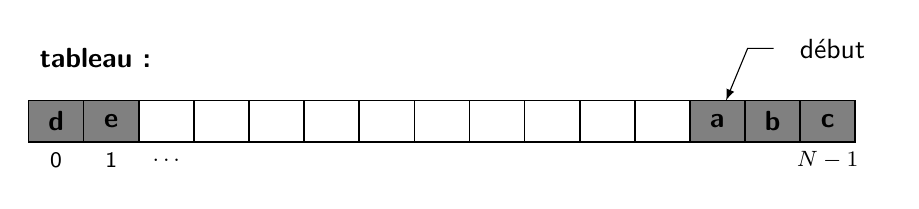
\begin{tikzpicture}[>=latex,font=\sffamily,every node/.style={minimum width=.7cm,minimum height=1.5em,outer sep=0pt,draw=black,fill=white,semithick}]
        \node at (0,0) (A) {};
        \foreach \L/\next in {A/B,B/C,C/D,D/E,E/F,F/G,G/H,H/I,I/J,J/K,K/L,L/M,M/N,N/O}{
        \node [anchor=west] at (\L.east) (\next) {};
        }
        \node[fill=gray] at (M) {\textbf{a}};
        \node[fill=gray] at (N) {\textbf{b}};
        \node[fill=gray] at (O) {\textbf{c}};
        \node[fill=gray] at (A) {\textbf{d}};
        \node[fill=gray] at (B) {\textbf{e}};
        \path (A) ++(0,-.5cm) node[draw=none,fill=none]   {\footnotesize 0};
        \path (B) ++(0,-.5cm) node[draw=none,fill=none]   {\footnotesize 1};
        \path (C) ++(0,-.5cm) node[draw=none,fill=none]   {\footnotesize $\ldots$};
        \path (O) ++(0,-.5cm) node[draw=none,fill=none]   {\footnotesize $N-1$};
        \path (B) ++(-.2cm,.8cm) node[draw=none,fill=none]   {\textbf{tableau :}};
        \draw [<-] (M) -- ++(67.5:1cm) -- +(.33cm,0)  node [right,inner xsep=.333cm,fill=none,draw=none] (Head) {\red{début}};
\end{tikzpicture}

 \end{frame}

\begin{frame}{File: mise en {\oe}uvre à l’aide d'un tableau}

\begin{tabbing}
  aaa\=aaa\=\kill
  \red{Enfiler}($x$) \\
  \uncover<2->{
    \>  \textbf{si} $lg = N$ \textbf{alors} \textsl{afficher} \texttt{erreur:file pleine} \\
    \>  \textbf{sinon} $T[(deb+lg) \mod N] \leftarrow x$; $lg \leftarrow lg + 1$;  \\
    \>  \textbf{fin si}}
  \end{tabbing}

~\\

\begin{tabbing}
  aaa\=aaa\=\kill
  \red{Défiler}() \\
  \uncover<3->{
    \> \textbf{si} $lg = 0$ \textbf{alors} \textsl{afficher} \texttt{erreur:file vide} \\
    \> \textbf{sinon} \= $lg \leftarrow lg - 1$; $y \leftarrow T[deb]$;\\\> \> $deb \leftarrow (deb+1) \mod N$; \\
   \>\>    \textsl{retourner} $y$ \\
    \> \textbf{fin si}}
\end{tabbing}

~\\
\begin{tabbing}
  aaa\=aaa\=\kill
  \red{EstVide}() \\
  \uncover<4->{
    \> \textsl{retourner} $lg = 0$}
\end{tabbing}
~\\
\end{frame}

\begin{frame}{File: mise en {\oe}uvre à l’aide d'un tableau}

\begin{tabbing}
  aaa\=aaa\=\kill
  \red{EstVide}() \\
  \uncover<4->{
    \> \textsl{retourner} $lg = 0$}
\end{tabbing}
~\\
\end{frame}


\begin{frame}{Liste}
Séquence finie d'éléments à laquelle on peut ajouter ou retirer  un  élément à  n'importe quelle place.
 
  \begin{itemize}
  \item $L =  (a,c,d,e,f,g,h)$
  \end{itemize}
  éventuellement vide :
  \begin{itemize}
  \item $L = () = \epsilon$
  \end{itemize}
\end{frame}

\begin{frame}
  \frametitle{Liste : quelques opérations de base}
 % $\mathbf{L =  (a,c,d,e,f,g,h)}$ \hfill $\mathbf{L' =  (u,v,w,x,z)}$
  \begin{itemize}
   \item<1-> \red{creerListeVide}() retourne une liste vide
  \item<2->  \red{estVide}(\textbf{L}) retourne vrai si la liste est  vide, faux sinon.
  \item<3-> \red{élément($p,\mathbf{L}$)} retourne l’élément en position $p$; $p$ doit être une place de $\mathbf{L}$.  
  \item<4-> \red{insérerElément($x,i,\mathbf{L}$)} retourne $\mathbf{L}$ avec l'élément $x$ en position $i$, les éléments initialement en position $p\geq i$ sont décalés à la position $p+1$ respectivement.
   \item<5-> \red{supprimerElément($i,\mathbf{L}$)} supprime et retourne l'élément de $\mathbf{L}$ à la position $i$. 
  %\item<5-> \red{insérertête($x,\mathbf{L}$) retourne \mathbf{L} avec l'élément $x$ ajouté en tête.
 \item<6-> \red{queue}($\mathbf{L}$) retourne la liste privée de sa tête (premier élément de $\mathbf{L}$)%$= (c,d,e,f,g,h)$ 
\item<7-> \red{tête}($\mathbf{L}$) retourne le premier élément de la liste $\mathbf{L}$ ($\mathbf{L}$ est inchangée)
\item<8-> \red{concaténation}($\mathbf{L}$,$\mathbf{L'}$) ($\mathbf{L} \mathbf{\circ} \mathbf{L'}$) retourne la liste $\mathbf{L}$ formée des éléments de $\mathbf{L}$ avant la concatenation suivis des éléments de $\mathbf{L'}$
% \item<6-> \red{longueur}(\textbf{L}) $= 7$. Nombre d'éléments dans la liste. Longueur($\epsilon$) $=0$. 
  \end{itemize}
\end{frame}

\begin{frame}
  \frametitle{Recherche dans une liste}
  Rechercher un élément dans une liste
  \begin{itemize}
  \item[] \underline{entrées} : liste \textbf{L}, élément \textbf{x}
  \item[] \underline{sortie} : vrai si $x \in L$, faux sinon
  \end{itemize}

  \begin{tabbing}
    aaa\=aaa\=aaa\kill
    \textbf{Rechercher}(L,x) \\
    \uncover<2->{\> \textbf{si} \red{estVide}(L) $\,$ \= \textbf{alors} \textsl{retourner} \textbf{faux} \textbf{fin si} \\}
    \uncover<3->{\> \textbf{si} \red{tête}(L) $= x$ \> \textbf{alors} \textsl{retourner} \textbf{vrai} \\}
    \uncover<4->{\>\> \textbf{sinon} \textsl{retourner} \textbf{Rechercher}(\red{queue}($L$),x) \\
     \> \textbf{fin si}}
  \end{tabbing}

 % \uncover<5->{Complexité $= $}\uncover<6->{\red{$\mathbf{O(n)}$} où $\mathbf{n}$ est la longueur de la liste.}   
\end{frame}

\begin{frame}
  \frametitle{Renverser une liste}
    \begin{itemize}
    \item[] \underline{entrées} : liste \textbf{L}
    \item[] \underline{sortie} :  liste contenant les éléments de \textbf{L} en ordre inverse
    \end{itemize}
    Exemple : \textbf{Renverser}(\textbf{(a,c,d,e,f,g,h)}) $ = $ \textbf{(h,g,f,e,d,c,a)}
    
  \begin{tabbing}
    aaa\=aaa\=aaa\kill
    \textbf{Renverser}(L) \\
    \uncover<2->{\> \textbf{si} \red{estVide}(L) \= \textbf{alors} \textsl{retourner} L \\}
    \uncover<3->{\> \textbf{sinon} \textsl{retourner} \red{concaténer}(\textbf{Renverser}(\red{queue}(L)),(\red{tête}(L)))  \\
     \> \textbf{fin si}}
  \end{tabbing}

 % \uncover<4->{Complexité $= $}\uncover<5->{\red{$\mathbf{O(n)}$} où $\mathbf{n}$ est la longueur de la liste.}   
\end{frame}

\begin{frame}
  \frametitle{Insertion dans une liste triée}
    \begin{itemize}
    \item[] \underline{entrées} : liste triée \textbf{L}, élément $\mathbf{x}$
    \item[] \underline{sortie} :  liste triée contenant les éléments de \textbf{L} et \textbf{x}
    \end{itemize}
    Exemple : \textbf{Insérer}(\textbf{(a,c,d,e,f,g,h)},\textbf{\red{b}}) $ = $ \textbf{(a,\textbf{\red{b}},c,d,e,f,g,h)}
    
  \begin{tabbing}
    aaa\=aaa\=aaa\kill
    \textbf{Insérer}(L,x) \\
    \uncover<2->{\> \textbf{si} \red{estVide}(L) $\;$\= \textbf{alors} \textsl{retourner} $\mathbf{(x)}$ \textbf{fin si}\\}
    \uncover<3->{\> \textbf{si} $x <$ \red{tête}(L) \textbf{alors} \textsl{retourner} \red{concaténer}(\textbf{(x)},\textbf{L})  \\}
      \uncover<4->{\> \textbf{sinon} \textsl{retourner} \red{concaténer}(\textbf{(}\red{tête}(L)\textbf{)},\textbf{Insérer}(\red{queue}(L),\textbf{x})) \\
     \> \textbf{fin si}}
  \end{tabbing}

 % \uncover<5->{Complexité $= $}\uncover<6->{\red{$\mathbf{O(n)}$} où $\mathbf{n}$ est la longueur de la liste.}     
\end{frame}


\tikzstyle{ptr}  = [draw, -latex',thick]
\tikzstyle{head} = [rectangle, draw, text height=3mm, text width=3mm, text centered, node distance=3cm, inner sep=0pt]
\tikzstyle{data} = [rectangle split, rectangle split parts=2, draw,
  text centered, minimum height=3em]


\begin{frame} \frametitle{Listes -- Mise en {\oe}uvre}
Plusieurs implémentations des listes sont possibles; le choix de l’implémentation dépend des opérations effectivement utilisées. \\

\emph{Implémentation par un tableau} : une place correspond à un indice, et la liste est conservée dans les premiers emplacements du tableau. Une variable supplémentaire tient à jour la longueur de la liste. \\
Certaines opérations seront simples et peu coûteuses à implementer (e.g.; \red{élément($p,\mathbf{L}$)}), d'autres  demanderont des décalages dans le tableau (e.g.\red{supprimerElément($i,\mathbf{L}$)}).
\end{frame}


\begin{frame} \frametitle{Listes -- Mise en {\oe}uvre}

\emph{Implémentation par listes chaînées} :
Chaque élément de la liste est représenté par un couple $(cont,succ)$ où $cont$ est du type des éléments de la liste et $succ$ indique (donne l'adresse de) l'élément suivant dans la liste. Pour le dernier élément $succ$ vaut $null$. 
La  tète  de  liste  contient  l'adresse  du  premier  élément. \\

Dans une liste chaînée nous n'avons pas d'accès direct à un élément, la liste doit être parcourue, élément par élément. Par contre elle permet une gestion dynamique de l'espace mémoire.

\end{frame}

\begin{frame}
%  \frametitle{Listes -- Mise en {\oe}uvre}
  Chaînage: 
  \begin{tikzpicture}[node distance=2cm, auto]
    %%% from stackoverflow http://tex.stackexchange.com/questions/93942/typesetting-classical-data-structures-in-tikz
    \node[head, label=below:\textbf{L}] (head) {};
    \node[data, right of=head]    (A) {\ldata[\textbf{a}]};
    \node[data, right of=A]       (B) {\ldata[\textbf{c}]};
    \node[data, right of=B]       (C) {\ldata[\textbf{d}]};
%    \node[above of=C,head,node distance=2cm,label=above:prev]   (prev){};
    \node[data, right of=C]       (D) {\ldata[\textbf{e}]};
%    \node[above of=D,head,node distance=2cm,label=above:curr]   (curr){};
    \node[data, right of=D]       (E) {\textbf{f}  \nodepart{second} null};
%    \node[data, right of=E]       (last) {data \nodepart{second} null};

    \draw[fill] (head.center)   circle (0.05);
%%    \draw[fill] (prev.center)   circle (0.05);
%%    \draw[fill] (curr.center)   circle (0.05);

    \path[ptr]  (head.center) --++(right:7.5mm)  |- (A.text west);
    \draw[fill] ($(A.south)!0.5!(A.text split)$) circle (0.05);
    \draw[ptr]  ($(A.south)!0.5!(A.text split)$) --++(right:10mm) |- (B.text west);
    \draw[fill] ($(B.south)!0.5!(B.text split)$) circle (0.05);
    \draw[ptr]  ($(B.south)!0.5!(B.text split)$) --++(right:10mm) |- (C.text west);
%%    \path[ptr] (prev) -- (C);
    \draw[fill] ($(C.south)!0.5!(C.text split)$) circle (0.05);
    \draw[ptr]  ($(C.south)!0.5!(C.text split)$) --++(right:10mm) |- (D.text west);
%%    \path[ptr] (curr) -- (D);
    \draw[fill] ($(D.south)!0.5!(D.text split)$) circle (0.05);
    \draw[ptr]  ($(D.south)!0.5!(D.text split)$) --++(right:10mm) |- (E.text west);
 %   \draw[fill] ($(E.south)!0.5!(E.text split)$) circle (0.05);
%    \draw[ptr]  ($(E.south)!0.5!(E.text split)$) --++(right:10mm) |- (last.text west);

\end{tikzpicture}
~\\~\\~\\
\uncover<2>{
  \begin{tikzpicture}[node distance=2cm, auto]
    %%% from stackoverflow http://tex.stackexchange.com/questions/93942/typesetting-classical-data-structures-in-tikz
    \node[head, label=below:\textbf{L},draw=none] (head) {};
    \node[data, right of=head, label=above:$x$]    (A) {\ldata[\textbf{a}]};
    \node[data, right of=A, label=above:$y$]       (B) {\textbf{c}  \nodepart{second} null};
%    \node[data, right of=E]       (last) {data \nodepart{second} null};

%%    \draw[fill] (head.center)   circle (0.05);
%%    \draw[fill] (prev.center)   circle (0.05);
%%    \draw[fill] (curr.center)   circle (0.05);

    \path[ptr,dotted]  (head.center) --++(right:7.5mm)  |- (A.text west);
    \draw[fill] ($(A.south)!0.5!(A.text split)$) circle (0.05);
    \draw[ptr,CadetBlue]  ($(A.south)!0.5!(A.text split)$) --++(right:10mm) |- (B.text west);
%    \draw[fill] ($(B.south)!0.5!(B.text split)$) circle (0.05);
%    \draw[ptr]  ($(B.south)!0.5!(B.text split)$) --++(right:10mm) |- (C.text west);
%%    \path[ptr] (prev) -- (C);
    \node[right=1.6cm of B] {\begin{tabular}{ll}
        \red{x.val} = \textbf{\red{a}} &  \blue{x.succ} = y \\
        \red{y.val} = \textbf{\red{c}} &  \blue{y.succ} = null
      \end{tabular}    };
\end{tikzpicture}}

\end{frame}

\begin{frame}
  \frametitle{Parcours de listes chaînées}
ex: longueur d'une liste
  \begin{itemize}
  \item[] \underline{entrées} : liste \textbf{L}
  \item[] \underline{sortie} : nombre d'élément de \textbf{L}, 0 si \textbf{L} est vide
  \end{itemize}

  \begin{tabbing}
    aaa\=aaa\=aaa\kill
    \textbf{Longueur}(L) \\
    \> crt $\leftarrow$ \textbf{L}; lgr $\leftarrow$ 0 \\
    \> \textbf{tant que} $crt \neq $ null \textbf{faire} \\
    \> \> $lgr \leftarrow lgr + 1$; \\
    \> \> $crt \leftarrow crt.succ$; \\
    \> \textbf{fin tant que} \\
    \> \textsl{retourner} lgr
  \end{tabbing}
  
\end{frame}

\begin{frame}
  \frametitle{Longueur d'une liste}

  \begin{tabbing}
    aaa\=aaa\=aaa\kill
    \textbf{Longueur}(L) \\
    \> crt $\leftarrow$ \textbf{L}; lgr $\leftarrow$ 0 \\
    \> \textbf{tant que} $crt \neq $ null \textbf{faire} \\
    \> \> $lgr \leftarrow lgr + 1$; \\
    \> \> $crt \leftarrow crt.succ$; \\
    \> \textbf{fin tant que} \\
    \> \textsl{retourner} lgr
  \end{tabbing}


  \begin{tikzpicture}[node distance=2cm, auto]
    %%% from stackoverflow http://tex.stackexchange.com/questions/93942/typesetting-classical-data-structures-in-tikz
    \node[head, label=below:\textbf{L}] (head) {};
    \node[head, label=below:\blue{\textbf{crt}},below=1.7cm of head]    (crt) {};
    \draw[fill] (crt.center)   circle (0.05);
    \node[right=3cm of crt] (lgr) {\textbf{lgr} $=$};
    \node[right=.1cm of lgr, visible on=<1>] {0};
    \node[right=.1cm  of lgr, visible on=<2>] {1};
    \node[right=.1cm  of lgr, visible on=<3>] {2};
    \node[right=.1cm of lgr, visible on=<4>] {3};
    \node[right=.1cm of lgr, visible on=<5>] {4};
    \node[right=.1cm  of lgr, visible on=<6>] {5};
    \node[data, right of=head]    (A) {\ldata[\textbf{a}]};
    \node[data, right of=A]       (B) {\ldata[\textbf{c}]};
    \node[data, right of=B]       (C) {\ldata[\textbf{d}]};
    \node[data, right of=C]       (D) {\ldata[\textbf{e}]};
    \node[data, right of=D]       (E) {\textbf{f}  \nodepart{second} null};
    \path[ptr, visible on=<1>, CadetBlue]  (crt.center) --++(right:7.5mm) --++(up:7.5mm) -| (A.south);
    \path[ptr, visible on=<2>, CadetBlue]  (crt.center) --++(right:7.5mm) --++(up:7.5mm) -| (B.south);
    \path[ptr, visible on=<3>, CadetBlue]  (crt.center) --++(right:7.5mm) --++(up:7.5mm) -| (C.south);
    \path[ptr, visible on=<4>, CadetBlue]  (crt.center) --++(right:7.5mm) --++(up:7.5mm) -| (D.south);
    \path[ptr, visible on=<5>, CadetBlue]  (crt.center) --++(right:7.5mm) --++(up:7.5mm) -| (E.south);
    \node[right=.1cm of crt,visible on=<6>] {$=$ null};

    \draw[fill] (head.center)   circle (0.05);
    \path[ptr]  (head.center) --++(right:7.5mm)  |- (A.text west);


    \draw[fill] ($(A.south)!0.5!(A.text split)$) circle (0.05);
    \draw[ptr]  ($(A.south)!0.5!(A.text split)$) --++(right:10mm) |- (B.text west);
    \draw[fill] ($(B.south)!0.5!(B.text split)$) circle (0.05);
    \draw[ptr]  ($(B.south)!0.5!(B.text split)$) --++(right:10mm) |- (C.text west);
    %% \path[ptr] (prev) -- (C);
    \draw[fill] ($(C.south)!0.5!(C.text split)$) circle (0.05);
    \draw[ptr]  ($(C.south)!0.5!(C.text split)$) --++(right:10mm) |- (D.text west);
    %% \path[ptr] (curr) -- (D);
    \draw[fill] ($(D.south)!0.5!(D.text split)$) circle (0.05);
    \draw[ptr]  ($(D.south)!0.5!(D.text split)$) --++(right:10mm) |- (E.text west);
    % \draw[fill] ($(E.south)!0.5!(E.text split)$) circle (0.05);
    % \draw[ptr]  ($(E.south)!0.5!(E.text split)$) --++(right:10mm) |- (last.text west);

\end{tikzpicture}  
\end{frame}

% ============================================
%============================================
\lecture{Graphes}{lec-graphe}
%============================================
%============================================
\begin{frame}
  \frametitle{Graphe}
  Un graphe $G = (V,E)$ se compose 
  \begin{itemize}
  \item<1-> d'un ensemble de \red{\textbf{sommets}} $V$ et
  \item<2-> d'un ensemble d'\blue{\textbf{arêtes}} $E$
  \end{itemize}

\uncover<3->{  exemple: $\red{\mathbf{V}} = \{1,2,3,4,5\}$ \\} \uncover<4->{ $~~~~~~~~~~~~\blue{\mathbf{E}} = \{\{1,2\}, \{1,5\}, \{2,3\}, \{2,5\}, \{3,4\}, \{4,5\} \}$
}
\begin{center}
    \begin{tikzpicture}[>=stealth',auto,node distance=1.8cm, very thick,
      main node/.style={visible on=<3->, circle,fill=BrickRed!90,draw,font=\sffamily\bfseries},
      every edge/.style={visible on=<4->, draw,very thick,CadetBlue}]

      \node[main node] (1) {1};
      \node[main node] (2) [below right of=1] {2};
      \node[main node] (3) [below  of=2] {3};
      \node[main node] (5) [below left  of=1] {5};
      \node[main node] (4) [below of=5] {4};

      
      \path[every node/.style={font=\sffamily\small}]
      (1) edge[CadetBlue] node [left] {} (2)
          edge  node[left] {} (5)
      (2) edge node [right] {} (3)
          edge node {} (5)
      (3) edge node [right] {} (4)
      (4) edge node [left] {} (5);
\end{tikzpicture}
\end{center}
\end{frame}

\begin{frame}
  \frametitle{Graphe orienté}
  Graphe orienté:
  \begin{itemize}
  \item ensemble de sommets \red{\textbf{V}} et
  \item ensemble d'\blue{\textbf{arcs A}} : arêtes orientées
  \end{itemize}

\uncover<2->{  exemple: $\red{\mathbf{V}} = \{1,2,3,4,5\}$ \\} \uncover<4->{ $~~~~~~~~~~~~\blue{\mathbf{A}} = \{(1,2), (1,5), (2,3), (2,5), (5,2), (3,4), (4,5) \}$
}
\begin{center}
  \begin{tikzpicture}[>=stealth',auto,node distance=1.8cm, very thick,
    main node/.style={visible on=<3->, circle,fill=BrickRed!90,draw,font=\sffamily\bfseries},
    every edge/.style={visible on=<4->, draw,very thick,CadetBlue,->,shorten >=1pt}]

      \node[main node] (1) {1};
      \node[main node] (2) [below right of=1] {2};
      \node[main node] (3) [below  of=2] {3};
      \node[main node] (5) [below left  of=1] {5};
      \node[main node] (4) [below of=5] {4};

      
      \path[every node/.style={font=\sffamily\small}]
      (1) edge[bend left] node [above] {} (2)
          edge[bend right]  node[above] {} (5)
      (2) edge node [right] {} (3)
          edge [bend right] node {} (5)
      (3) edge [bend left]node [right] {} (4)
      (4) edge node [left] {} (5)
      (5) edge [bend right] node {} (2);
    \end{tikzpicture}
  \end{center}
\end{frame}

\begin{frame}
  \frametitle{Applications}
  \begin{itemize}
  \item Modélisation/analyse de réseaux informatiques, sociaux, biologiques, etc.
  \item Analyse/conception de circuits
  \item Navigation, calcul de plus courts trajets
  \item Ordonnancement, emploi du temps
  \item Classement de pages web
  %\item Structure des langues
  \item $\ldots$
  \end{itemize}
\end{frame}


\begin{frame}{Coloriage}
  \begin{minipage}{0.4\linewidth}
  \includegraphics[clip=true, trim=4.8cm 3cm 3cm 4.3cm, scale=.3]{sam3.pdf}    
  \end{minipage}
  \begin{minipage}{0.58\linewidth}
    \only<1>{\includegraphics{amsud-graph}}
    \only<2->{\includegraphics{amsud-graph-color}}
  \end{minipage}

\end{frame}
\begin{frame}
  \frametitle{Plus court chemin}
\centering
  \includegraphics[scale=.4,clip=true,trim= 10cm 1cm 5cm 10cm]{trajet}
\end{frame}

\begin{frame}
  \frametitle{Graphe de pages web}
  \includegraphics[scale=2.72]{wikipedia-toppages}

  \hfill \tiny{source: \url{https://flic.kr/p/bJEQWe}}
\end{frame}

\begin{frame}
  \frametitle{Communautés}
  \includegraphics[scale=.11]{wikipedia_socialgraph.jpg}

  \hfill \tiny{source: \url{https://flic.kr/p/afsXkh}}
\end{frame}

\begin{frame}
  \frametitle{Représentation des graphes}
  \begin{enumerate}
  \item<1-> Matrice d'adjacence
  \item<2-> Liste d'adjacence 
  \end{enumerate}
\end{frame}

\begin{frame}
  \frametitle{Matrice d'adjacence}
  $\mathbf{G} = (V,E)$ avec $V = \{1,\ldots,n\}$
~\\
  \red{\textbf{M}} \red{matrice d'adjacence} de G:
  \begin{itemize}
  \item taille $n \times n$
  \item $M[i,j] = \left\{
      \begin{array}{ll}
        1 & \mbox{si $\{i,j\}$ \blue{arête} de G} \\
        0 & \mbox{sinon}
      \end{array}
    \right.$ 
  \end{itemize}
  \begin{minipage}{.48\linewidth}
\begin{center}
  \begin{tikzpicture}[>=stealth',auto,node distance=1.8cm, very thick,
    main node/.style={ circle,fill=BrickRed!90,draw,font=\sffamily\bfseries}
]

      \node[main node] (1) {1};
      \node[main node] (2) [below right of=1] {2};
      \node[main node] (3) [below  of=2] {3};
      \node[main node] (5) [below left  of=1] {5};
      \node[main node] (4) [below of=5] {4};
      \draw[very thick,black]
      (1) edge node [left] {} (2)
          edge node [left] {} (5)
      (2) edge node [right] {} (3)
%      (3) edge node [right] {} (4)
      (4) edge node [left] {} (5);
      \path[visible on=<1>,black, very thick] 
      (2) edge (5);
      \path[visible on=<1-2>,black, very thick] 
      (3) edge (4);
      \path[visible on=<2->,line width=2pt,color=CadetBlue]
      (5) edge (2);
      \path[visible on=<3>,line width=2pt,color=OliveGreen]
      (3) edge (4);
\end{tikzpicture}
\end{center}    
  \end{minipage}
  \begin{minipage}{.48\linewidth}
    $$
    \mathbf{M} = \left[
    \begin{array}{ccccc}
      0 & 1 & 0 & 0 & 1 \\
      1 & 0 & 1 & 0 & \only<1>{1}\only<2->{\blue{\mathbf{1}}} \\
      0 & 1 & 0 & \only<1-2>{1}\only<3->{\green{\mathbf{1}}} & 0 \\
      0 & 0 & \only<1-2>{1}\only<3->{\green{\mathbf{1}}} & 0 & 1 \\
      1 & \only<1>{1}\only<2->{\blue{\mathbf{1}}} & 0 & 1 & 0
    \end{array}
    \right]
    $$
  \end{minipage}
\end{frame}

\begin{frame}
  \frametitle{Listes d'adjacences}
  À chaque sommet $i$ est associé la \red{\textbf{liste de ses
      voisins}}

~\\~\\
  \begin{minipage}{.48\linewidth}
\begin{center}
  \begin{tikzpicture}[>=stealth',auto,node distance=1.8cm, very thick,
    main node/.style={ circle,fill=BrickRed!90,draw,font=\sffamily\bfseries}
]

      \node[main node] (1) {1};
      \node[main node] (2) [below right of=1] {2};
      \node[main node] (3) [below  of=2] {3};
      \node[main node] (5) [below left  of=1] {5};
      \node[main node] (4) [below of=5] {4};
      \draw[very thick,black]
      (1) edge node [left] {} (2)
      (2) edge node [right] {} (3)
      (3) edge node [right] {} (4);
      \path[visible on=<1>,black, very thick] 
      (5) edge (2)
          edge (1)
          edge (4);
      \path[visible on=<2->,line width=2pt,color=CadetBlue]
      (5) edge (2)
          edge (1)
          edge (4);
    \end{tikzpicture}
\end{center}    
  \end{minipage}
  \begin{minipage}{.48\linewidth}
    $$
    \begin{array}{c|l}
      \mbox{sommet} & \mbox{liste} \\
      \hline
      1 & (2,5) \\
      2 & (1,5,3) \\
      3 & (2,4) \\
      4 & (3,5) \\
      \only<1>{5}\only<2>{\red{\mathbf{5}}} & \only<1>{(1,2,4)}\only<2>{\blue{\mathbf{(1,2,4)}}}
    \end{array}
    $$
  \end{minipage}
\end{frame}

\begin{frame}
  \frametitle{Matrice \emph{vs} Listes d'adjacences}
  
Soit $G = (\mathbf{V},\mathbf{E})$ un graphe. Quelle représentation
choisir ?
~\\~\\

\begin{tabular}{l|cc}
  & \red{Matrice} & \blue{Listes} \\
  \hline
  $\exists ? ~~(u,v)$ & \uncover<2->{$O(1)$} & \uncover<3->{$> O(1)$} \\
Espace total & \uncover<4->{$O(|V|^2)$} & \uncover<5->{$O( |E|)$}
\end{tabular}
~\\~\\
\uncover<6->{\begin{minipage}{.38\linewidth}
~\\~\\
  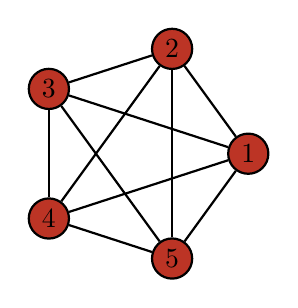
\begin{tikzpicture}
    \foreach \x in {1,...,5}{%
      \pgfmathparse{(\x-1)*360/5}
      \node[draw,circle,inner sep=0.08cm,fill=BrickRed!90] (\x) at (\pgfmathresult:1.4cm) [thick] {\x};
    }
    \foreach \x in {1,...,5}{%
      \foreach \y in {\x,...,5}{%
        \path (\x) edge[thick,-] (\y);
      }
    }
  \end{tikzpicture}
  \centering
  \uncover<7->{$\red{|E|} = \mathbf{O(|V|^2)}$}
\end{minipage}
\begin{minipage}{.6\linewidth}
  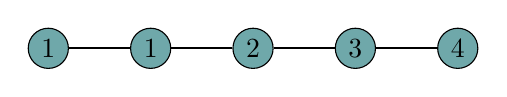
\begin{tikzpicture}[node distance=1.3cm]
    \node[draw,circle,inner sep=0.08cm,fill=CadetBlue!90] (N0) {1};
    \foreach \x/\y in {1/0,2/1,3/2,4/3}{%
      \node[draw,circle,inner sep=0.08cm,fill=CadetBlue!90] (N\x)
      [right of=N\y] {\x};
      \path (N\y) edge[thick,-] (N\x);
    }
  \end{tikzpicture}
  \centering
  \uncover<8->{$\blue{|E|} = \mathbf{O(|V|)}$}
\end{minipage}}
\end{frame}

\begin{frame}
  \frametitle{Chaînes}
  Soit $s,t$ deux sommets. Une \red{\textbf{chaîne}} est une suite
  d'arêtes consécutive reliant $s$ à $t$. 

  ~\\~\\
  \begin{minipage}{.48\linewidth}
    \begin{center}
      \begin{tikzpicture}[>=stealth',auto,node distance=1.8cm, very thick,
        main node/.style={ circle,fill=BrickRed!90,draw,font=\sffamily\bfseries},
        other node/.style={ circle,fill=white,draw}]
        \node[main node] (1) {1};
        \node[other node] (2) [below right of=1] {2};
        \node[main node] (3) [below  of=2] {3};
        \node[other node] (5) [below left  of=1] {5};
        \node[other node] (4) [below of=5] {4};
        \draw[very thick,black]
           (5) edge (2);
        \path[visible on=<1>,black, very thick] 
           (1) edge (5)
           (5) edge (4)
           (4) edge  (3);
         \path[visible on=<1-2>,black, very thick] 
           (1) edge  (2)
           (2) edge  (3);
         \path[visible on=<2->,line width=2pt,color=CadetBlue]
           (1) edge (5)
           (5) edge (4)
           (4) edge  (3);
         \path[visible on=<3->,line width=2pt,color=OliveGreen]
           (1) edge  (2)
           (2) edge  (3);
            \end{tikzpicture}
          \end{center}    
        \end{minipage}
  \begin{minipage}{.48\linewidth}
    chaînes des sommets  $\red{\mathbf{1}}$ à $\red{\mathbf{3}}$:
    \begin{itemize}
    \item<2-> $\blue{\{1,5\},\{5,4\},\{4,3\}}$
    \item<3-> $\green{\{1,2\},\{2,3\}}$
    \item<4-> $\ldots$
    \end{itemize}
  \end{minipage}

\end{frame}

\begin{frame}
  \frametitle{Distance}
  La \red{\textbf{distance}} entre deux sommets $u,v$ est le \textbf{nombre d'arêtes} dans une \textbf{plus petite chaîne} reliant $u$ à $v$.
  ~\\~\\
  \begin{minipage}{.48\linewidth}
    \begin{center}
      \begin{tikzpicture}[>=stealth',auto,node distance=1.8cm, very thick,
        main node/.style={ circle,fill=BrickRed!90,draw,font=\sffamily\bfseries},
        other node/.style={ circle,fill=white,draw}]
        \node[other node] (1) {1};
        \node[other node] (2) [below right of=1] {2};
        \node[other node] (3) [below  of=2] {3};
        \node[other node] (5) [below left  of=1] {5};
        \node[other node] (4) [below of=5] {4};
        \path[black, very thick] 
           (1) edge[CadetBlue,line width=2pt] (5)
           (5) edge (2)
           (5) edge[BrickRed,line width=2pt] (4)
           (4) edge[BrickRed,line width=2pt]  (3)
           (1) edge[OliveGreen,line width=2pt]  (2)
           (2) edge[OliveGreen,line width=2pt]  (3);
         \end{tikzpicture}
          \end{center}    
        \end{minipage}
  \begin{minipage}{.48\linewidth}

    \begin{align*}
      \blue{dist(1,5)} & = 1 \\
      \red{dist(5,3)} & = 2 \\
      \green{dist(1,3)} & = 2
    \end{align*}
  \end{minipage}
\end{frame}


\begin{frame}
  \frametitle{Calcul des distances}
  \begin{itemize}
  \item[] \underline{entrées} : graphe $\mathbf{G} = (V,E)$, sommet $\mathbf{s} \in V$
  \item[] \underline{sortie} : tableau $\mathbf{dist}$ des distances à partir de $s$  \\
    $~~~~~~~~~\forall u \in V, \mathbf{dist}[u] = $ distance de $s$ à $u$ dans $\mathbf{G}$
  \end{itemize}
  ~\\~\\
  \uncover<2->{
    \begin{minipage}{.46\linewidth}
      \begin{tikzpicture}[>=stealth',auto,node distance=1.4cm,very thick,
    main/.style={circle,fill=BrickRed!90,draw,font=\footnotesize\sffamily\bfseries},
    other/.style={circle,fill=white,draw,font=\footnotesize}]
    \node[other] (F) {F};
    \node[other] (E) [right of=F] {E};
    \node[main] (S) [right of=E] {S};
    \node[other] (A) [right of=S] {A};
    \node[other] (B) [below of=A] {B};
    \node[other] (C) [left of=B] {C};
    \node[other] (D) [left of=C] {D};
    \draw
    (A) edge (B)
        edge (S)
    (B) edge (C)
    (C) edge (S)
    (D) edge (E)
        edge (S)
    (E) edge (S)
        edge (F);
  \end{tikzpicture}
\end{minipage}
}
\uncover<4->{
  \begin{minipage}{.48\linewidth}
    \includegraphics[scale=1]{distance-graph}
  \end{minipage}
}
\uncover<3->{
  \begin{tabular}{c|cccccc}
 sommet & A & B & C & D & E & F \\
    \hline
   distance& 1 & 2 & 1 & 1 & 1 & 2 
  \end{tabular}
}
\end{frame}

\begin{frame}
  \frametitle{Calcul des distances}
  Procéder \emph{couche par couche}
  \begin{itemize}
  \item<2-> Couche $\blue{\mathbf{d}}$ : sommets à distance $\blue{\mathbf{d}}$
  \item<3-> Couche $\green{\mathbf{d+1}}$ : sommets 
    \begin{itemize}
    \item<4-> $\notin$ couches $0,\ldots,\blue{\mathbf{d}}$ et
    \item<4-> adjacents aux sommets de la couche $\blue{\mathbf{d}}$
    \end{itemize}
  \end{itemize}
~\\~\\
  \begin{minipage}{.48\linewidth}
    \includegraphics[scale=.8]{distance-graph-color}
  \end{minipage}
\end{frame}

\begin{frame}
  \frametitle{Parcours en largeur}
Algorithme itératif
\begin{itemize}
\item<1-> À tout moment 2 couches actives 
  \begin{enumerate}
  \item<2-> couche \blue{\textbf{d}}, précédemment complètement identifiée
  \item<3-> couche \green{\textbf{d+1}}, en cours d'identification (à l'aide de la couche \blue{\textbf{d}})
  \end{enumerate}
\item<4-> Structure de données adaptée ?? \uncover<5->{\red{$\longrightarrow$ File}}
\end{itemize}
\end{frame}
\begin{frame}
  \frametitle{Parcours en largeur}
  \framesubtitle{Breadth-First Search}

  \begin{tabbing}
    aa\=aa\=aaa\=aaa\=aaa\=\kill
    \textbf{ParcoursEnLargeur}(G = (V,E),s) \hfill \texttt{/* G graphe, s sommet */}\\
    \> $dist \leftarrow$ CréerTableau($|V|$) \\
    \> $Q \leftarrow$ CréerFileVide() \\
    \> \textbf{pour chaque} $u \in V$ \textbf{faire} $dist[u] \leftarrow +\infty$ \textbf{fin pour} \\
    \> $dist[s] \leftarrow 0$; $Enfiler(Q,s)$ \\~\\

    \> \textbf{tant que} EstNonVide($Q$) \textbf{faire} \\
    \> \> $u \leftarrow$ Défiler($Q$) \\
    \> \> \textbf{pour chaque} arête $\{u,v\}$ \textbf{faire} \\
    \> \> \> \textbf{si} $dist[v] = +\infty$ \textbf{alors} $dist[v] \leftarrow dist[u]+1$; Enfiler($Q,v$) \\    \> \> \> \textbf{fin si} \\
    \>\> \textbf{fin pour} \\
    \> \textbf{fin tant que} \\
    \> \textsl{retourner} $dist$
  \end{tabbing}
\end{frame}

\begin{frame}
  \frametitle{Parcours en largeur : exemple}
  entrée :
      \begin{tikzpicture}[>=stealth',auto,node distance=1.4cm,very thick,
    main/.style={circle,fill=BrickRed!90,draw,font=\footnotesize\sffamily\bfseries},
    other/.style={circle,fill=white,draw,font=\footnotesize}]
    \node[other] (F) {F};
    \node[other] (E) [right of=F] {E};
    \node[main] (S) [right of=E] {S};
    \node[other] (A) [right of=S] {A};
    \node[other] (B) [below of=A] {B};
    \node[other] (C) [left of=B] {C};
    \node[other] (D) [left of=C] {D};
    \draw
    (A) edge (B)
        edge (S)
    (B) edge (C)
    (C) edge (S)
    (D) edge (E)
        edge (S)
    (E) edge (S)
        edge (F);
    \node[other,fill=CadetBlue,visible on=<6->] at (A) {A};
    \node[other,fill=CadetBlue,visible on=<7->] at (C) {C};
    \node[other,fill=CadetBlue,visible on=<8->] at (D) {D};
    \node[other,fill=CadetBlue,visible on=<9->] at (E) {E};
    \node[other,fill=CadetBlue,visible on=<10->] at (B) {B};
    \node[other,fill=CadetBlue,visible on=<11->] at (F) {F};
  \end{tikzpicture}

~\\~\\~\\
  \begin{tabular}{c|c}
    Ordre de visite & File \\
    \hline 
      & $[ S ]$ \\
    \uncover<1->{S} & \only<2>{$[A]$}\only<3>{$[C,A]$}\only<4>{$[D,C,A]$}\only<5->{$[E,D,C,A]$} \\
      \uncover<6->{ A & $[B,E,D,C]$ \\}
    \uncover<7->{ C & $[B,E,D]$ \\}
    \uncover<8->{ D & $[B,E]$ \\}
    \uncover<9->{ E & $[F,B]$ \\}
    \uncover<10->{ B & $[F]$ \\}
    \uncover<11->{ F & $[]$}
  \end{tabular}
\end{frame}

\begin{frame}
  \frametitle{Parcours en largeur : analyse}
  \underline{Complexité} : \uncover<4->{$\red{\mathbf{O(|V|+|E|)}}$}
  \begin{itemize}
  \item<2-> Chaque sommet mis en file \textbf{exactement une fois} \\
    \hfill $\red{\longrightarrow \mathbf{2|V|}}$ opérations sur la file
  \item<3-> Chaque arête est parcourue $\red{\mathbf{2}}$ fois 
    \hfill $\red{\longrightarrow \mathbf{2|E|}}$ opérations 
  \end{itemize}
~\\
  \uncover<5->{\underline{Correction} : }
  \begin{itemize}
  \item<6->[] Montrer que. pour chaque $d=0,1,\ldots$, il existe un état dans lequel sont vérifiées :
    \begin{enumerate}
    \item pour chaque sommet $u$ à distance $d^{'}\leq d$, $dist[u]=d^{'}$
    \item pour tout autre sommet $v$, $dist[v] = +\infty$
    \item la file contient exactement les sommets à distance $d$.
    \end{enumerate}
  \end{itemize}
\end{frame}


\begin{frame}
  \frametitle{Graphes pondérés}
  \begin{center}
    \includegraphics[width=.8\linewidth]{villes-graph}
  \end{center}
% \begin{itemize}
%  \item[] Chaque arête est munie d'un \red{\emph{poids positif}} (distance, coût,...)
% % \item [] Le poids d’une chaîne est la somme des poids des arêtes qui la composent.
%  \item[] Une plus courte chaîne entre deux sommets est, parmi les chaînes qui les relient, une chaîne de poids minimum.
%  \end{itemize}   
\end{frame}


\begin{frame}
  \frametitle{Plus courtes chaînes dans les graphes pondérés}
  \begin{itemize}
 \item[] Chaque arête est munie d'un \red{\emph{poids positif}} (distance, coût,...)
  \item [] Le poids d’une chaîne est la somme des poids des arêtes qui la composent.
 \item[]  \red{\emph{Une plus courte chaîne}} entre deux sommets est, parmi les chaînes qui les relient, une chaîne de poids minimum.
 \end{itemize}   
\end{frame}

\begin{frame}
  \frametitle{Plus courtes chaînes dans les graphes pondérés}
  \begin{itemize}
  \item[] \underline{entrées} : graphe $\mathbf{G} = (V,E)$ pondéré, sommet
    $\mathbf{s} \in V$
  \item[] \underline{sortie} : tableau $\mathbf{dist}$ des distances à partir de $s$  \\
    $~~~~~~~~~\forall u \in V, \mathbf{dist}[u] = $ distance de $s$ à $u$ dans $\mathbf{G}$
  \end{itemize}
  \uncover<2->{\underline{Notation}: pour chaque arête $e = \{u,v\} \in
    E$,  \\
    \hspace{1.6cm} soit \red{$\mathbf{\ell(e)} = \mathbf{\ell(\{u,v\})}$} le poids de
    l'arête $e$ }

  \uncover<3->{~\\\underline{Hypothèse}: tous les poids sont
    \red{\emph{positifs}}, i.e., $\forall e \in E, \ell(e) > 0$. }
\end{frame}

\begin{frame}
  \frametitle{Plus courtes chaînes dans les graphes pondérés}
  \begin{itemize}
  \item[] \underline{entrées} : graphe $\mathbf{G} = (V,E)$ pondéré, sommet
    $\mathbf{s} \in V$
  \item[] \underline{sortie} : tableau $\mathbf{dist}$ des distances à partir de $s$  \\
    $~~~~~~~~~\forall u \in V, \mathbf{dist}[u] = $ distance de $s$ à $u$ dans $\mathbf{G}$
  \end{itemize}

    %\begin{center}
  \begin{minipage}{.56\linewidth}
      \begin{tikzpicture}[>=stealth',auto, very thick,
        main node/.style={circle,fill=BrickRed!90,draw,font=\sffamily\bfseries},
        other node/.style={ circle,fill=white,draw},
        lnode/.style=CadetBlue,font=\bfseries]
        \begin{scope}[node distance=1.2cm and 2.5cm,on grid]
          \node[main node] (A)  {A};
          \node[other node] (B) [above right= of A]{B};
        \node[other node] (C) [right= of B] {C};
        \node[other node] (E) [below right= of A]  {E};
        \node[other node] (D) [right= of E] {D};
        \path[black, very thick] 
        (A) edge node[below,CadetBlue,font=\bfseries] {2} (E)
                edge node[above,lnode] {1}(B)
            (B) edge node[above,lnode]{4}(C)
                edge node[right,lnode]{3}(E)
                edge node[above,lnode]{2}(D)
            (C) edge node[right,lnode]{1}(D)
            (D) edge node[above,lnode]{1}(E);
      \end{scope}
    \end{tikzpicture}
  \end{minipage}
  \begin{minipage}[t]{.23\linewidth}
    \uncover<2->{
      \begin{tabular}{r|cccc}
        $u$ & B & C & D & E \\
        \hline
        dist(\red{A},$u$) & 1 & 4 & 3 & 2 
   \end{tabular}
}
\end{minipage}
\end{frame}

\begin{frame}
  Parcours en largeur (BFS) : le poids de chaque arête est
  $\mathbf{\blue{1}}$

\uncover<2->{\textbf{G}
%  \begin{minipage}{.56\linewidth}
      \begin{tikzpicture}[>=stealth',auto, very thick,
        main node/.style={circle,fill=BrickRed!90,draw,font=\sffamily\bfseries},
        other node/.style={ circle,fill=white,draw},
        lnode/.style=CadetBlue,font=\bfseries]
        \begin{scope}[node distance=1.2cm and 2.5cm,on grid]
          \node[main node] (A)  {A};
          \node[other node] (B) [above right= of A]{B};
        \node[other node] (C) [right= of B] {C};
        \node[other node] (E) [below right= of A]  {E};
        \node[other node] (D) [right= of E] {D};
        \path[black, very thick] 
        (A) edge node[below,CadetBlue,font=\bfseries] {2} (E)
                edge node[above,lnode] {1}(B)
            (B) edge node[above,lnode]{4}(C)
                edge node[right,lnode]{3}(E)
                edge node[above,lnode]{2}(D)
            (C) edge node[right,lnode]{1}(D)
            (D) edge node[above,lnode]{1}(E);
        \node[draw=none] (L) [visible on=<4->,right=8.5cm of A] {\parbox{4cm}{$\forall u \in
          \{B,C,D,E\}$ $\mathbf{dist_G(A,u) = \red{dist_{G'}(A,u)}}$}};
      \end{scope}
    \end{tikzpicture} 
 % \end{minipage}
}
\uncover<3->{
~\\\red{\textbf{G'}}
    \begin{tikzpicture}[>=stealth',auto, very thick,
      main node/.style={circle,fill=BrickRed!90,draw,font=\sffamily\bfseries},
      other node/.style={ circle,fill=white,draw,font=\bfseries},
      lnode/.style={CadetBlue,font=\bfseries},
      dummy/.style={circle,minimum width=.3cm,fill=white,draw=black}]
      \begin{scope}[node distance=1.8cm and 4.5cm,on grid]
        \node[main node] (A)  {A};
        \node[other node] (B) [above right= of A]{B};
        \node[other node] (C) [right= of B] {C};
        \node[other node] (E) [below right= of A]  {E};
        \node[other node] (D) [right= of E] {D};
      \path[black, very thick] 
      (A) edge  (E)
      edge (B)
      (B) edge (C)
      edge (E)
      edge (D)
      (C) edge (D)
      (D) edge (E);
        % A -- E
        \node[dummy] at (barycentric cs:A=.5,E=.5) {};
        % B -- E
        \node[dummy] at (barycentric cs:B=.33,E=.66) {};
        \node[dummy] at (barycentric cs:B=.66,E=.33) {};
        % B -- D 2 
        \node[dummy] at (barycentric cs:B=.5,D=.5) {};
        % B -- C 4
        \node[dummy] at (barycentric cs:B=.25,C=.75) {};
        \node[dummy] at (barycentric cs:B=.5,C=.5) {};
        \node[dummy] at (barycentric cs:B=.75,C=.25) {};
      \end{scope}        
      \end{tikzpicture}}
  \end{frame}

  \begin{frame}
    ~\\
    \begin{tikzpicture}[>=stealth',auto, very thick,
      main node/.style={circle,fill=BrickRed!90,draw,font=\sffamily\bfseries},
      other node/.style={ circle,fill=white,draw,font=\bfseries},
      lnode/.style={CadetBlue,font=\bfseries},
      dummy/.style={circle,minimum width=.3cm,fill=white,draw=black}]
      \begin{scope}[node distance=1.8cm and 4.5cm,on grid]
        \node[main node] (A)  {A};
        \node[other node] (B) [above right= of A]{B};
        \node[other node] (C) [right= of B] {C};
        \node[other node] (E) [below right= of A]  {E};
        \node[other node] (D) [right= of E] {D};
      \path[black, very thick] 
      (A) edge  (E)
      edge (B)
      (B) edge (C)
      edge (E)
      edge (D)
      (C) edge (D)
      (D) edge (E);
        % A -- E
        \node[dummy] at (barycentric cs:A=.5,E=.5) {};
        % B -- E
        \node[dummy] at (barycentric cs:B=.33,E=.66) {};
        \node[dummy] at (barycentric cs:B=.66,E=.33) {};
        % B -- D 2 
        \node[dummy] at (barycentric cs:B=.5,D=.5) {};
        % B -- C 4
        \node[dummy] at (barycentric cs:B=.25,C=.75) {};
        \node[dummy] at (barycentric cs:B=.5,C=.5) {};
        \node[dummy] at (barycentric cs:B=.75,C=.25) {};
      \end{scope}        
      \end{tikzpicture}
      Construction de $\red{\mathbf{G'}}$
      \begin{itemize}
      \item<2-> Remplacer chaque arête $e$ de \textbf{G} par $\ell(e)$
        arêtes en ajoutant $\ell(e)-1$ sommets
      \end{itemize}
      Calcul des distance dans $G$ 
      \begin{itemize}
      \item<3->[] $\red{\mathbf{\longrightarrow}}$  Parcours en largeur dans $\red{\mathbf{G'}}$
    \end{itemize}
  \end{frame}

  \begin{frame}
    Calcul des distances dans $\red{\mathbf{G'}}$: %\uncover<2->{\textbf{Inefficace}}

    \begin{tikzpicture}[>=stealth',auto, very thick,
      main node/.style={circle,fill=BrickRed!90,draw,font=\sffamily\bfseries},
      other node/.style={ circle,fill=white,draw,font=\bfseries},
      lnode/.style={CadetBlue,font=\bfseries},
      dummy/.style={circle,minimum width=.3cm,fill=white,draw=black},
      node distance=1cm and 2.5cm,on grid]
      \node[main node] (A)  {A};
      \node[other node] (B) [above right= of A]{B};
      \node[other node] (C) [below right= of A]{C};
      \node[right=-1cm of A] {\textbf{G}};
      \path[black, very thick] 
      (A) edge node[lnode] {100} (B) 
          edge node[below,lnode] {200} (C)
       (B)   edge node[right,lnode] {50} (C);  
     \end{tikzpicture}

    \begin{tikzpicture}[>=stealth',auto,  
      main node/.style={circle,fill=BrickRed!90,draw,font=\sffamily\bfseries},
      other node/.style={circle,fill=white,draw,font=\bfseries},
      lnode/.style={CadetBlue,font=\bfseries},
      dummy/.style={circle,minimum
        width=.2cm,fill=white,draw=black,inner sep=0},
      node distance=1cm and 7.5cm,on grid]
      \node[main node] (A)  {A};
      \node[other node] (B) [above right= of A]{B};
      \node[] (Cdum) [below right= of A]{};
      \node[other node] (C) [right=2cm of Cdum]{C};
      \node[right=-1cm of A,BrickRed] {\textbf{G'}};
      \node[dummy] (Bnd) at (barycentric cs:A=.5,B=.5) {};
      \node[dummy] (Cnd) at (barycentric cs:A=.52,C=.48) {};
      \node[dummy] (X) at (barycentric cs:B=.70,C=.30) {};
      \node[dummy] (Y) at (barycentric cs:C=.70,B=.30) {};
      \path[black] 
        (A) edge   (Bnd) 
            edge   (Cnd)
       (Bnd) edge[dashed] (B)
       (Cnd) edge[dashed] (C)
        (B)  edge  (X)
        (C) edge (Y)
        (X) edge[dashed] (Y);

      \node[dummy] (B1) at (barycentric cs:A=.90,B=.1) {};
      \node[dummy] (B2) at (barycentric cs:A=.80,B=.2) {};
      \node[dummy] (B3) at (barycentric cs:A=.70,B=.3) {};
      \node[dummy] (B4) at (barycentric cs:A=.60,B=.4) {};
      \node[dummy] (C1) at (barycentric cs:A=.92,C=.08) {};
      \node[dummy] (C2) at (barycentric cs:A=.84,C=.16) {};
      \node[dummy] (C3) at (barycentric cs:A=.76,C=.24) {};
      \node[dummy] (C4) at (barycentric cs:A=.68,C=.32) {};
      \node[dummy] (C5) at (barycentric cs:A=.6,C=.4) {};

      \node[dummy,visible on=<2->,fill=CadetBlue,label=above:\footnotesize{\onslide<2->{1}}] at (B1) {};
      \node[dummy,visible on=<2->,fill=CadetBlue,label=below:\footnotesize{\onslide<2->{1}}] at (C1) {};
      \node[dummy,visible on=<3->,fill=CadetBlue,label=above:\footnotesize{\onslide<3->{2}}] at (B2) {};
      \node[dummy,visible on=<3->,fill=CadetBlue,label=below:\footnotesize{\onslide<3->{2}}] at (C2) {};
      \node[dummy,visible on=<4->,fill=CadetBlue,label=above:\footnotesize{\onslide<4->{3}}] at (B3) {};
      \node[dummy,visible on=<4->,fill=CadetBlue,label=below:\footnotesize{\onslide<4->{3}}] at (C3) {};
      \node[dummy,visible on=<5->,fill=CadetBlue,label=above:\footnotesize{\onslide<5->{4}}] at (B4) {};
      \node[dummy,visible on=<5->,fill=CadetBlue,label=below:\footnotesize{\onslide<5->{4}}] at (C4) {};
     \end{tikzpicture}

     \begin{itemize}
       \item<2-> Calcul de distances pour de nombreux sommets non pertinents
       \item<2-> Attente avant de connaître les distances dans $G$ \\
%         dépend des poids 
     \end{itemize}
   \end{frame}



%  \begin{frame}
%    \begin{tikzpicture}[>=stealth',auto, thick,
%      main node/.style={circle,fill=BrickRed!90,draw,inner sep=2pt},
%      other node/.style={ circle,fill=white,draw,inner sep=2pt},
%      lnode/.style={CadetBlue,font=\footnotesize},
%      dummy/.style={circle,minimum width=.3cm,fill=white,draw=black},
%      node distance=.6cm and 2.2cm,on grid]
%      \node[main node] (A)  {A};
%      \node[other node] (B) [above right= of A]{B};
%      \node[other node] (C) [below right= of A]{C};
%      \node[right=-1cm of A] {\textbf{G}};
%      \path[black,  thick] 
%      (A) edge node[lnode] {100} (B) 
%          edge node[below,lnode] {200} (C)
%       (B)  edge node[right,lnode] {50} (C);  
%     \end{tikzpicture}
%
%    \begin{tikzpicture}[>=stealth',auto,  
%      main node/.style={circle,fill=BrickRed!90,draw,font=\sffamily,inner sep=2pt},
%      other node/.style={circle,fill=white,draw,inner sep=2pt},
%      lnode/.style={CadetBlue,font=\footnotesize},
%      dummy/.style={circle,minimum
%        width=.2cm,fill=white,draw=black,inner sep=0},
%      node distance=.8cm and 5.5cm,on grid]
%      \node[main node] (A)  {A};
%      \node[other node] (B) [above right= of A]{B};
%      \node[] (Cdum) [below right= of A]{};
%      \node[other node] (C) [right=2cm of Cdum]{C};
%      \node[right=-1cm of A,BrickRed] {\textbf{G'}};
%      \node[dummy] (Bnd) at (barycentric cs:A=.5,B=.5) {};
%      \node[dummy] (Cnd) at (barycentric cs:A=.52,C=.48) {};
%      \node[dummy] (X) at (barycentric cs:B=.70,C=.30) {};
%      \node[dummy] (Y) at (barycentric cs:C=.70,B=.30) {};
%      \path[black] 
%        (A) edge   (Bnd) 
%            edge   (Cnd)
%       (Bnd) edge[dashed] (B)
%       (Cnd) edge[dashed] (C)
%        (B)  edge  (X)
%        (C) edge (Y)
%        (X) edge[dashed] (Y);
%
%      \node[dummy] (B1) at (barycentric cs:A=.90,B=.1) {};
%      \node[dummy] (B2) at (barycentric cs:A=.80,B=.2) {};
%      \node[dummy] (B3) at (barycentric cs:A=.70,B=.3) {};
%      \node[dummy] (B4) at (barycentric cs:A=.60,B=.4) {};
%      \node[dummy] (C1) at (barycentric cs:A=.92,C=.08) {};
%      \node[dummy] (C2) at (barycentric cs:A=.84,C=.16) {};
%      \node[dummy] (C3) at (barycentric cs:A=.76,C=.24) {};
%      \node[dummy] (C4) at (barycentric cs:A=.68,C=.32) {};
%      \node[dummy] (C5) at (barycentric cs:A=.6,C=.4) {};
%
%      \node[dummy,visible on=<1->,fill=CadetBlue,label=above:\tiny{1}] at (B1) {};
%      \node[dummy,visible on=<1->,fill=CadetBlue,label=below:\tiny{1}] at (C1) {};
%      \node[dummy,visible on=<1->,fill=CadetBlue,label=above:\tiny{2}] at (B2) {};
%      \node[dummy,visible on=<1->,fill=CadetBlue,label=below:\tiny{2}] at (C2) {};
%      \node[dummy,visible on=<1->,fill=CadetBlue,label=above:\tiny{3}] at (B3) {};
%      \node[dummy,visible on=<1->,fill=CadetBlue,label=below:\tiny{3}] at (C3) {};
%      \node[dummy,visible on=<1->,fill=CadetBlue,label=above:\tiny{4}] at (B4) {};
%      \node[dummy,visible on=<1->,fill=CadetBlue,label=below:\tiny{4}] at (C4) {};
%     \end{tikzpicture}
%
%     \underline{Supp.} parcours d'une unité de distance par minute
%     \begin{itemize}
%     \item<2-> Sommet \textbf{A} atteint au bout de 100 minutes
%     \item<3->[] $\red{\longrightarrow}$ Alarme associé à chaque sommet $v$ \\ $~~~~$= temps estimé pour atteindre $v$
%     \item<4-> initialement
%       \begin{tabular}{l|ccc}
%         & A & B & C \\
%         \hline
%         \blue{\textbf{\clock}} & 0 & 100 & 200
%       \end{tabular}
%     \item<5-> à $T=100$,  une fois B atteint 
%       \begin{tabular}{l|ccc}
%         & A & B & C\\
%         \hline
%         \blue{\textbf{\clock}} & 0  & 100 & \blue{\textbf{150}}
%       \end{tabular}
%     \end{itemize}
%   \end{frame}
%
%   \begin{frame}{Algorithme : esquisse}
%     à chaque sommet $u$ est associé une alarme $\blue{\mathbf{alarme}}(u)$ \\
%     \begin{tabbing}
%       aaa\=aaa\=aaa\=\kill
%       \uncover<2->{CalculDistance(s,G) \\}
%       \uncover<3->{\> Initialement:  $\blue{\mathbf{alarme}}(s) = 0$; $\blue{\mathbf{alarme}}(u) = +\infty$ pour $u\neq s$;  \\~\\}
%       \uncover<3->{\> \textbf{tant qu}'il existe des alarmes actives \textbf{faire}\\
%         \> \> supp. que l'alarme du sommet \textbf{u} soit la prochaine  à sonner \\
%         \> \>  au temps $\blue{\mathbf{T}}$ alors : \\}
%       \uncover<4->{\> \> \red{1)} \textbf{dist}(s,u) = T \\}
%       \uncover<5->{\> \> \red{2)} \textbf{pour chaque} voisin $v$ de $u$ \textbf{faire} \\
%         \> \> \> $\blue{\mathbf{alarme}}(u) = \min(\mathbf{alarme}(u),T+\ell(\{u,v\}))$ \\
%       \> \textbf{fin tant que}}
%     \end{tabbing}
%   \end{frame}

%   \begin{frame}
%     \frametitle{Gestion des alarmes : \\ structure de données}
%     Quelle structure de données pour gérer les alarmes ? \\
%     
%     ~\\
%     \uncover<6->{\red{\textbf{File de priorités}}}
%~\\
%     \underline{Opérations} :
%     \begin{itemize}
%     \item<2-> \red{Insérer}($v$,\blue{T}): insère  $v$ avec alarme qui sonne à $T$
%     \item<3-> \red{SupprimerMin}(): supprime l'élément qui a la plus petite alarme et le retourne
%     \item<4-> \red{EstVide}(): retourne vrai si l'ensemble est vide, faux sinon
%     \item<5-> \red{DiminuerAlarme}(v,\blue{T'}): règle l'alarme de $v$ pour sonner à $T'$ 
%     \end{itemize}
%   \end{frame}

   \begin{frame}
     \frametitle{File de priorité}
 Une file de priorité permet de gérer un ensemble d’éléments, dont chacun a une valeur associée  baptisée \emph{clé} qui denote la priorité de l'élément.\\ Dans une file de priorité min, plus petite est la clé d'un élément plus grande est sa priorité. \\ 
   \underline{Opérations pour file de priorité min }:
   \begin{itemize}
     \item \red{Insérer}(F,$v$,\blue{T}): insère  $v$ avec clé  $T$
     \item \red{SupprimerMin}(F): supprime et retourne l'élément qui a la plus petite clé 
     \item \red{EstVide}(F): retourne \emph{vrai} si F  est vide, \emph{faux} sinon
     \item \red{AugmenterPriorité}(F,v,\blue{T'}): diminue la valeur de la \emph{clé} de $v$ en lui donnant la valeur $T'$
     \item \red{CreerFilePriorité}(): crée une file de priorité vide 
     \end{itemize}
 \end{frame}

   \begin{frame}
     \frametitle{Algorithme de Dijkstra}
     \subtitle{Calcul de plus courtes chaînes}
     \begin{tabbing}
       aaa\=aaa\=aaaaaaaaaaaa\=\kill
       \textbf{dijkstra}($G,\ell,s$) \texttt{/* G= (V,E) graphe (orienté ou non)} \\
       \>\>\> \texttt{$\ell:E \rightarrow \mathbb{R}^{+}$ pondération des arêtes} \\
       \>\>\> \texttt{$s\in V$ */} \\
       \> $H \leftarrow$ \red{CreerFilePriorité}() \\
       \> \textbf{pour chaque} $u \in V$ \textbf{faire} \\
       \> \ $dist[u] \leftarrow \blue{\mathbf{+\infty}}$; $prev[u]\leftarrow null$; \red{Insérer}($H,u,dist[u]$)    \\ \> \textbf{fin pou} \\
        \>  $dist(s) \leftarrow$ 0;\\
       \> \red{AugmenterPriorité}($H,s,\blue{0}$) \\
       \> \textbf{tant que} \red{EstNonVide}(H) \textbf{faire} \\
       \> \> $u \leftarrow$ \red{SupprimerMin}(H) \\
       \> \> \textbf{pour}\= \textbf{ chaque} arête $(u,v)$ \textbf{faire} \\
       \> \> \> \textbf{si} \=$dist[v] > dist[u]+ \ell(u, v)$ \textbf{alors} \\
       \> \> \> \> $dist[v] \leftarrow dist[u]+ \ell(u, v)$; $ prev[v] \leftarrow u$ \\
       \> \> \> \> \red{AugmenterPriorité}(H,v,dist[v])  \textbf{fin si}\\
       \> \textsl{retourner} dist
     \end{tabbing}
   \end{frame}

%   \begin{frame}
%     \frametitle{Algorithme de Dijkstra : exemple}
%     \begin{tikzpicture}[>=stealth',auto,thick,
%       main/.style={circle,draw=BrickRed!90,font=\sffamily\bfseries,inner sep=2pt,thick},
%       other/.style={circle,fill=white,draw,inner sep=2pt},
%       done/.style={circle,fill=CadetBlue,draw,inner sep=2pt},
%       lnode/.style={font=\tiny}]
%       \begin{scope}[node distance=1.2cm and 2.5cm,on grid]
%         \node[main]  (A)  {A};
%         \node[other] (B) [above right= of A] {B};
%         \node[other] (C) [below right= of A] {C};
%         \node[other] (D) [right= of B]       {D};
%         \node[other] (E) [right= of C]       {E};
%         \path[black,->] 
%         (A) edge node[above,lnode] {4} (B)
%             edge[visible on=<1-2>] node[below,lnode] {2} (C)
%         (B) edge[bend right=20] node[left,lnode] {3} (C)
%             edge node[near end,lnode] {3} (E)
%             edge node[above,lnode] {2} (D)
%         (C) edge[bend right=20] node[right,lnode] {1} (B)
%             edge node[near end,lnode] {4} (D)
%             edge node[below,lnode] {5} (E)
%         (E) edge node[right,lnode] {1} (D);
%
%         
%         \node[done,visible on=<2->] at (A) {A};
%         \node[done,visible on=<3->] at (C) {C};
%         \node[done,visible on=<4->] at (B) {B};
%         \node[done,visible on=<5->] at (D) {D};
%         \node[done,visible on=<6->] at (E) {E};
%         \path[CadetBlue,->,very thick]
%         (A) edge[visible on=<3->] node[below,lnode] {2} (C)
%         (C) edge[bend right=20,visible on=<4->] node[right,lnode] {1} (B)
%         (B) edge[visible on=<5->] node[above,lnode] {2} (D)
%         (B) edge[visible on=<6->] node[near end,lnode] {3} (E);
%       \end{scope}
%    \end{tikzpicture} 
%~\\~\\
%    $H =$ \only<1>{$\{(A,0);(B,+\infty);(C,+\infty);(D,+\infty);(E,+\infty)\}$} 
%          \only<2>{$\{\mathbf{(B,4)};\mathbf{(C,2)};(D,+\infty);(E,+\infty)\}$} 
%          \only<3>{$\{\mathbf{(B,3)};\mathbf{(D,6)};\mathbf{(E,7)}\}$} 
%          \only<4>{$\{\mathbf{(D,5)};\mathbf{(E,6)}\}$} 
%          \only<5>{$\{(E,6)\}$} 
%          \only<6>{$\{\}$} 
%          ~\\~\\
%    \begin{tabular}{l|p{1cm}p{1cm}p{1cm}p{1cm}p{1cm}}
%      & A & B & C & D & E \\
%      \hline
%      $dist(A,\cdot{})$ & 
%      \only<1>{ 0}\only<2->{ \textbf{0}} & %A 
%      \only<1-3>{$+\infty$}\only<4->{\textbf{3}} & %B
%      \only<1-2>{$+\infty$}\only<3->{\textbf{2}} & %C
%      \only<1-4>{$+\infty$}\only<5->{\textbf{5}} & %D 
%      \only<1-5>{$+\infty$}\only<6->{\textbf{6}}  \\%E 
%         $prev$ & 
%      \only<1->{null} & %A 
%      \only<1>{null}\only<2>{A}\only<3->{C} & %B
%      \only<1>{null}\only<2->{A} & %C
%      \only<1-2>{null}\only<3>{C}\only<4->{B} & %D 
%      \only<1-2>{null}\only<3>{C}\only<4->{B}  %E 
%    \end{tabular} 
%   \end{frame}

   \begin{frame}
     \frametitle{Algorithme de Dijkstra : Complexité}
          \begin{tabbing}
       aa\=aa\=aaaaaaaaaaaa\=\kill
       \textbf{dijkstra}($G,\ell,s$) \\
       \> \textbf{pour chaque} $u \in V$ \textbf{faire} \\
       \> \> $dist(u) = \blue{\mathbf{+\infty}}$; $prev(u) = null$; \red{Insérer}($H,u,dist(u)$)         \textbf{fin pour} \\
       \>  $dist(s) \leftarrow 0$;\\
       \>  \red{AugmenterPriorité}($H,s,\blue{0}$) \\
       \> \textbf{tant que} \red{EstNonVide}(H) \textbf{faire} \\
       \> \> $u \leftarrow$ \red{SupprimerMin}(H) \\
       \> \> \textbf{pour}\= \textbf{ chaque} arête $(u,v)$ \textbf{faire} \\
       \> \> \> \textbf{si} \=$dist(v) > dist(u) + \ell(u, v)$ \textbf{alors} \\
       \> \> \> \> $dist(v) \leftarrow dist(u) + \ell(u, v)$; $ prev(v) \leftarrow u$ \\
       \> \> \> \> \red{AugmenterPriorité}(H,v,dist(v)) \textbf{fin si}
     \end{tabbing}
     nb. appels : \\ 
     \red{Insérer} : \uncover<2->{$\mathbf{|V|}$}
      \red{SupprimerMin} : \uncover<3->{$\mathbf{|V|}$}
      \red{AugmenterPriorité} : \uncover<4->{ $\mathbf{|E|}$}
     
     \uncover<5->{Tas : Insérer, SupprimerMin, AugmenterPriorité  $\mathbf{O(\log |V|)}$ \\
       Complexité(Dijkstra) = $\red{\mathbf{O((|E|+|V|)\log |V|)}}$}
   \end{frame}
   

% ============================================
%============================================
\lecture{Arbres}{lec-arbre}
%============================================
%============================================
\begin{frame}
  \frametitle{Définition}
  Un \red{arbre} est un \textbf{graphe connexe sans cycle} %\\
~\\~\\
Une \red{arborescence} est définie à partir d'un arbre en choisissant un sommet appelé \red{racine} et 
en orientant les arêtes de sorte qu'il existe un chemin de la racine vers tous les autres sommets.


\begin{tikzpicture}[every node/.style={circle,fill,draw,minimum width=3pt,thick},level distance=1cm]
    \node[fill=BrickRed] (Rac) {}
    child{ node[fill=OliveGreen] {}
       child{ node[fill=OliveGreen] {}
           child{ node[fill=CadetBlue] {}} }}
    child{ node[fill=CadetBlue] {}}
    child{ node[fill=OliveGreen] (L1) {}
       child{ node[fill=OliveGreen] (L2){} 
         child{ node[fill=CadetBlue] {}}
         child { node[fill=CadetBlue] {}}
         %child{ node[fill=OliveGreen] (L3) {}
            %   child { node[fill=CadetBlue] {}}
          %     child { node[fill=CadetBlue] {}}}
        % child{ node[fill=CadetBlue] {}}
       }}
    ;
    \node[fill=BrickRed] (LT1) [right=3.8cm of L1,label=right:\red{racine}] {};
%    \node[fill=CadetBlue] (LT2) [right=3.8cm of L2,label=right:\blue{feuille}] {};
%    \node[fill=CadetBlue] (LT3) [right=3.8cm of L3,label=right:\green{n\oe{}ud interne}] {};
  \end{tikzpicture}\end{frame}

\begin{frame}
  \frametitle{Vocabulaire :Ancêtres et descendants }
\begin{itemize}
\item Soit x un nœud d’un arbre T de racine r, un nœud y sur le chemin unique allant de r à x est appelé \emph{ancêtre} de x. x est un \emph{descendant} de y.
\item Pour tout arc $(y,x)\in T$, y est le \emph{père} de $x$ et $x$ est un \emph{fils} de $y$
\end{itemize}
\end{frame}


\begin{frame}
  \frametitle{Ancêtres et descendants}
\begin{tikzpicture}[every child node/.style={circle,fill,draw,minimum width=3pt,thick},level distance=1cm,
    tnode/.style={circle,fill,draw,minimum width=3pt,thick}]
    \node[tnode,fill=CadetBlue] (Rac) {}
    child{ node[fill=white] {}
       child{ node[fill=white] {}
           child{ node[fill=white] {}} }}
    child{ node[fill=white] {}}
    child{ node[fill=CadetBlue] (L1) {}
       child{ node[fill=BrickRed,inner sep=1pt] (L2){\textbf{v}} 
         child{ node[fill=OliveGreen] (fils1) {}}
         child{ node[fill=OliveGreen] (L3) {}
               child { node[fill=OliveGreen] {}}
               child { node[fill=OliveGreen] {}}}
         child{ node[fill=OliveGreen] (fils2) {}}
       }}
    ;
    \node[tnode,fill=CadetBlue] (LT1) [above right=1.8cm of L1,label=right:\blue{ancêtres} de \textbf{v}] {};
    \node[tnode,fill=OliveGreen] (LT2) [below =.2cm of LT1,label=right:\green{descendants} de \textbf{v}] {};
    \node (Lpere) [right=3cm of L1] {père de \textbf{v}};
    \node (Lfils) [right=3cm of L2] {fils de \textbf{v}};
    \path[->,draw]
    (Lfils) edge (fils1)
            edge (L3)
            edge (fils2)
    (Lpere) edge (L1);
  \end{tikzpicture}
~\\~\\
\underline{Propriété}: tout n\oe{u}d a au plus un père
\end{frame}


\begin{frame}
  \frametitle{Vocabulaire : racine, feuille, ...}
\begin{itemize}
\item La \emph{racine} est le seul nœud de T sans père
\item Deux nœuds avec le même père sont dits \emph{frères} 
\item Un nœud sans fils est dit \emph{feuille}
\item Un nœud qui n’est pas une feuille est dit \emph{nœud interne}
\end{itemize}
\end{frame}


\begin{frame}
  \frametitle{Vocabulaire racine, feuille, ...}
  \begin{tikzpicture}[every node/.style={circle,fill,draw,minimum width=3pt,thick},level distance=1cm]
    \node[fill=BrickRed] (Rac) {}
    child{ node[fill=OliveGreen] {}
       child{ node[fill=OliveGreen] {}
           child{ node[fill=CadetBlue] {}} }}
    child{ node[fill=CadetBlue] {}}
    child{ node[fill=OliveGreen] (L1) {}
       child{ node[fill=OliveGreen] (L2){} 
         child{ node[fill=CadetBlue] {}}
         child{ node[fill=OliveGreen] (L3) {}
               child { node[fill=CadetBlue] {}}
               child { node[fill=CadetBlue] {}}}
         child{ node[fill=CadetBlue] {}}
       }}
    ;
    \node[fill=BrickRed] (LT1) [right=3.8cm of L1,label=right:\red{racine}] {};
    \node[fill=CadetBlue] (LT2) [right=3.8cm of L2,label=right:\blue{feuille}] {};
    \node[fill=OliveGreen] (LT3) [right=3.8cm of L3,label=right:\green{n\oe{}ud interne}] {};
  \end{tikzpicture}
\end{frame}


\begin{frame}
  \frametitle{Hauteur et profondeur}
  \begin{minipage}{.32\linewidth}
  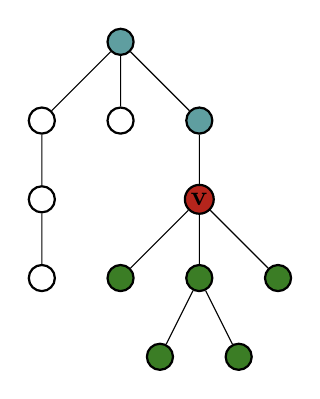
\begin{tikzpicture}[every child node/.style={circle,fill,draw,minimum width=3pt,thick},level distance=1cm,
    tnode/.style={circle,fill,draw,minimum width=3pt,thick},sibling distance=1.0cm]
    \node[tnode,fill=CadetBlue] (Rac) {}
    child{ node[fill=white] {}
       child{ node[fill=white] {}
           child{ node[fill=white] {}} }}
    child{ node[fill=white] {}}
    child{ node[fill=CadetBlue] (L1) {}
       child{ node[fill=BrickRed,inner sep=1pt] (L2){\textbf{v}} 
         child{ node[fill=OliveGreen] (fils1) {}}
         child{ node[fill=OliveGreen] (L3) {}
               child { node[fill=OliveGreen] {}}
               child { node[fill=OliveGreen] {}}}
         child{ node[fill=OliveGreen] (fils2) {}}
       }}
    ;
  \end{tikzpicture}    
  \end{minipage}
  \begin{minipage}{.66\linewidth}
    \red{profondeur d'un n{\oe}ud} $u$ = distance de $u$ à la racine \\~\\
     \red{hauteur d'un n{\oe}ud} $u$ = le nombre d’arcs du chemin le plus long qui le relie à une feuille \\~\\
    hauteur(racine) = 4 \\
    profondeur(\textbf{v}) = 2 
   \end{minipage}
~\\~\\    \red{hauteur d'un arbre} = hauteur de sa racine
\end{frame}

\begin{frame}
  \frametitle{Arbre binaire}
  
Tout n{\oe}ud a au plus \red{\textbf{2 fils}}


  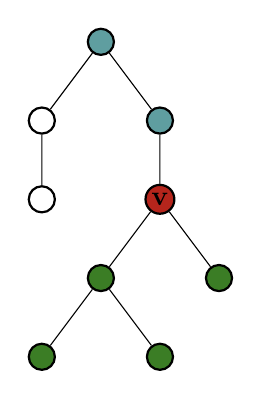
\begin{tikzpicture}[every child node/.style={circle,fill,draw,minimum width=3pt,thick},level distance=1cm,
    tnode/.style={circle,fill,draw,minimum width=3pt,thick}]
    \node[tnode,fill=CadetBlue] (Rac) {}
    child{ node[fill=white] {}
      child{ node[fill=white] {}
 %       child{ node[fill=white] {}} 
      }}
%    child{ node[fill=white] {}}
    child{ node[fill=CadetBlue] (L1) {}
       child{ node[fill=BrickRed,inner sep=1pt] (L2){\textbf{v}} 
         child{ node[fill=OliveGreen] (L3) {}
               child { node[fill=OliveGreen] {}}
               child { node[fill=OliveGreen] {}}}
         child{ node[fill=OliveGreen] (fils2) {}}
       }}
    ;
  \end{tikzpicture}
~\\
\uncover<2->{Arbre binaire \red{complet} : tout n{\oe}ud interne a exactement 2 fils}~\\~\\
\uncover<3->{Un arbre binaire \red{parfait} est un arbre binaire complet dans lequel toutes les feuilles sont à la même profondeur}.
~\\
\uncover<4->{ Le \red{nombre de n{\oe}uds} d'un arbre binaire parfait de \red{hauteur h} est }\uncover<4->{$\red{\mathbf{2^{h+1}-1}}$} 
\end{frame}


\begin{frame}
  \frametitle{Parcours en profondeur d'un arbre binaire}
\begin{itemize}
 \item \red{Parcours préfixe}, la racine d'un sous-arbre est visitée avant les éléments du sous-arbre gauche et du sous-arbre droit. \red{Parcours préfixe des sous-arbres gauche et droit}
\item \red{Parcours postfixe}, la racine d'un sous-arbre est visitée après les éléments du sous-arbre gauche et du sous-arbre droit. \red{Parcours postfixe des sous-arbres gauche et droit}
\item \red{Parcours infixe}, la racine d'un sous-arbre est visitée entre les éléments du sous-arbre gauche et du sous-arbre droit. \red{Parcours infixe des sous-arbres gauche et droit}
 \end{itemize}
  \end{frame}

%\begin{frame}
%  \frametitle{Arbres binaires de recherche}
%Dans un arbre binaire de recherche chaque nœud $x$ a une étiquette $l(x)$ (et une valeur associée) et satisfait la propriété suivante,\\
%Soit $L_G(x)$ et $L_D(x)$ les clés des nœuds du sous-abre gauche et du sous-abre droit de $x$ alors
%$\red{\forall y\in L_G(x) et z\in L_D(x),   y\geq l(x)<z}$  
%  \end{frame}
%
%\begin{frame}
%  \frametitle{Arbres binaires de recherche}
%Le \red{successeur d’un nœud} est le nœud possédant la plus petite étiquette supérieure à l'étiquette  de x 
%\end{frame}
%  
%\begin{frame}
%Théorème. 
%Les opérations Rechercher, Minimum, Maximum, Successeur et Prédécesseur peuvent se faire en temps O(h) sur un arbre binaire de recherche de hauteur h.
%\end{frame}

\begin{frame}
  \frametitle{Tas binaire (heap)}
  Arbre \red{quasi parfait}:
  \begin{itemize}
  \item Tous les niveaux sont pleins, à l'exception du dernier
  \item Le dernier niveau est rempli de gauche à droite
  \end{itemize}
  \red{Contrainte d'ordre (Tas min)}
  \begin{itemize}
  \item Valeur de chaque n{\oe}ud \red{$\mathbf{\leq}$} valeurs de ses fils 
  \end{itemize}
\red{Contrainte d'ordre (Tas max)}
  \begin{itemize}
  \item Valeur de chaque n{\oe}ud \red{$\mathbf{\geq}$} valeurs de ses fils 
  \end{itemize}
\end{frame}

\begin{frame}
  \frametitle{Tas binaire min}
  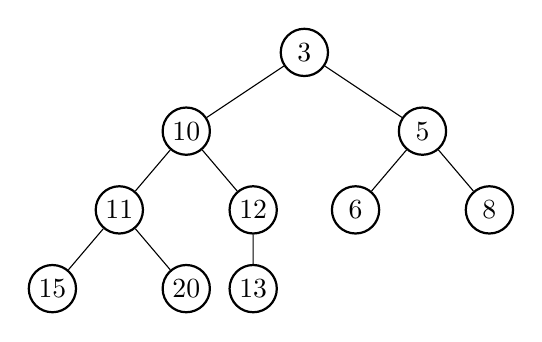
\begin{tikzpicture}[level distance=1cm,
    tnode/.style={circle,draw,minimum width=3pt,thick}]
    \tikzstyle{every node}=[circle,draw,minimum size=.6cm,thick,inner sep=1pt]
    \tikzstyle{level 1}=[sibling distance=30mm]
    \tikzstyle{level 2}=[sibling distance=17mm]
    \node (Rac) {3} %L0
    child{ node {10}       %L1
      child{ node {11}
        child{ node {15}}
        child{ node {20}}}
      child{ node {12}
        child{ node {13}}}}
    child{ node {5}     %L1
      child{ node {6}}  
      child{ node {8}}}
    ;
  \end{tikzpicture}
\end{frame}

\begin{frame}
  \frametitle{Insertion}
  Insérer n{\oe}ud avec valeur \red{\textbf{7}}:\\~\\

  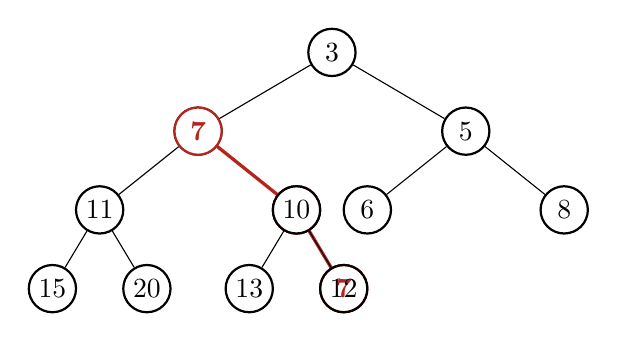
\begin{tikzpicture}[level distance=1cm,
    tnode/.style={circle,draw,minimum width=3pt,thick}]
    \tikzstyle{every node}=[circle,draw,minimum size=.6cm,thick,inner sep=1pt]
    \tikzstyle{level 1}=[sibling distance=34mm]
    \tikzstyle{level 2}=[sibling distance=25mm]
    \tikzstyle{level 3}=[sibling distance=12mm]
    \node (Rac) {3} %L0
    child{ node (F3) {10}       %L1
      child{ node {11}
        child{ node {15}}
        child{ node {20}}}
      child{ node (F2) {12}
        child{ node {13}}
        child{ node[BrickRed,visible on=<2>] (F1) {\textbf{7}}
          edge from parent[visible on=<2>, very thick, BrickRed]}
      }}
    child{ node {5}     %L1
      child{ node {6}}  
      child{ node {8}}}
    ;
    \path
    (F1) edge[visible on=<3->] (F2)
    (F2) edge[visible on=<4>,BrickRed,very thick] (F3);
    \node[visible on=<3->] at (F1) {12};
    \node[visible on=<3->,BrickRed,fill=white] at (F2) {\textbf{7}};
    \node[visible on=<5->,BrickRed,fill=white] at (F3) {\textbf{7}};
    \node[visible on=<5->,fill=white] at (F2) {10};
  \end{tikzpicture}
~\\~\\
\uncover<6->{Complexité:  }\uncover<7>{$\mathbf{\red{O(\log n)}}$ où $\mathbf{n}$ est le nombre de n\oe{}uds}
\end{frame}


\begin{frame}
  \frametitle{Suppression}
  Supprimer la \red{valeur minimale}

  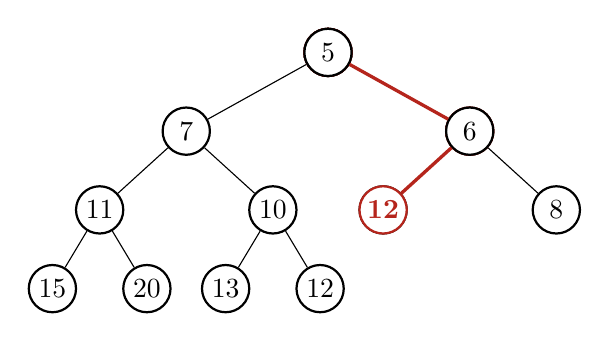
\begin{tikzpicture}[level distance=1cm,
    tnode/.style={circle,draw,minimum width=3pt,thick}]
    \tikzstyle{every node}=[circle,draw,minimum size=.6cm,thick,inner sep=1pt]
    \tikzstyle{level 1}=[sibling distance=36mm]
    \tikzstyle{level 2}=[sibling distance=22mm]
    \tikzstyle{level 3}=[sibling distance=12mm]
    \node (Rac) {3} %L0
    child{ node  {7}       %L1
      child{ node {11}
        child{ node {15}}
        child{ node {20}}}
      child{ node  {10}
        child{ node {13}}
        child{ node[visible on=<1-2>] {12} edge from parent[visible on=<1-2>]}
      }}
    child{ node (D1) {5}     %L1
      child{ node (D2) {6}}  
      child{ node {8}}}
    ;
    \node[visible on=<2>,fill=white] at (Rac) {};
    \node[visible on=<3-4>,BrickRed,fill=white] at (Rac) {\textbf{12}};
    \node[visible on=<5->,fill=white] at (Rac) {5};
    \node[visible on=<5-6>,BrickRed,fill=white] at (D1) {\textbf{12}};
    \node[visible on=<7->,BrickRed,fill=white] at (D2) {\textbf{12}};
    \node[visible on=<7->,fill=white] at (D1) {6};
    \path
    (Rac) edge[BrickRed,very thick,visible on=<4>] (D1)
    (D1) edge[BrickRed,very thick,visible on=<6>] (D2);
    
  \end{tikzpicture}
~\\~\\
\uncover<8->{Complexité:  }\uncover<9>{$\mathbf{\red{O(\log n)}}$ où $\mathbf{n}$ est le nombre de n\oe{}uds}
\end{frame}


\begin{frame}
  \frametitle{Diminution de la valeur d'un n\oe{}ud}
  Similaire à \red{Insertion}:
  \begin{enumerate}
  \item<2-> Modifier la valeur du n{\oe}ud
  \item<3-> Remonter au besoin la valeur pour respecter la contrainte d'ordre
  \end{enumerate}
\uncover<4->{Complexité:  $\mathbf{\red{O(\log n)}}$ où $\mathbf{n}$ est le nombre de n\oe{}uds}
\end{frame}

\begin{frame}
  \frametitle{Tas et tableau}
\only<1>{
  \begin{center}
    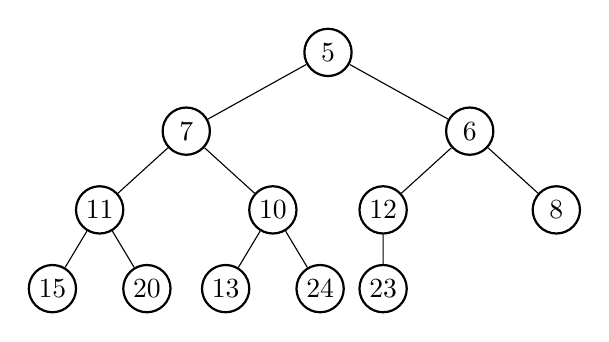
\begin{tikzpicture}[level distance=1cm,
      tnode/.style={circle,draw,minimum width=3pt,thick}]
      \tikzstyle{every node}=[circle,draw,minimum
      size=.6cm,thick,inner sep=1pt] \tikzstyle{level 1}=[sibling
      distance=36mm] \tikzstyle{level 2}=[sibling distance=22mm]
      \tikzstyle{level 3}=[sibling distance=12mm] \node[] (Rac)
      {5} %L0
      child{ node[] {7} %L1
        child{ node[] {11} child{ node[] {15}} child{ node[] {20}}}
        child{ node[] {10} child{ node[] {13}} child{ node[] {24}}}}
      child{ node[] (D1) {6} %L1
        child{ node[] (D2) {12} child{node[] {23}}} child{ node[] {8}
        }} ;
    \end{tikzpicture}
  \end{center}

  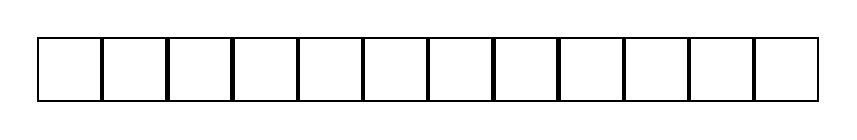
\begin{tikzpicture}
    [every node/.style={inner sep=4pt,draw,thick,minimum size=.8cm},%
    lineDecorate/.style={-,thick}]
%    \footnotesize
    \pgfmatrix{rectangle}{center}{}
    {\pgfusepath{}}{\pgfpointorigin}{\let\&=\pgfmatrixnextcell}
    {
      \node(0){}; \& \node(2){}; \& \node(3){}; \& \node(6){}; \&
      \node(4){}; \& \node(8){}; \& \node(10){}; \& \node(17){}; \&
      \node(13){}; \& \node(19){}; \& \node(24){}; \&
      \node(23){}; \\
    }
\end{tikzpicture}
}
\only<2>{
  \begin{center}
    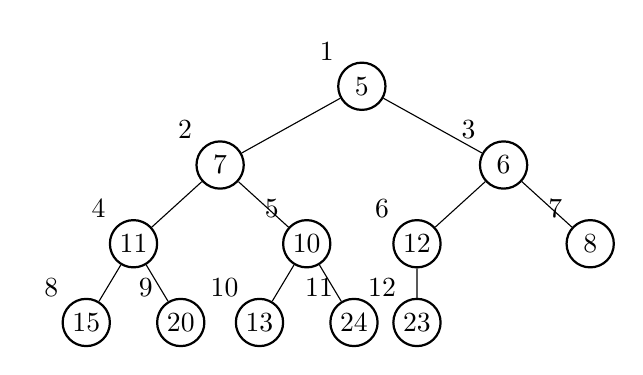
\begin{tikzpicture}[level distance=1cm,
      tnode/.style={circle,draw,minimum width=3pt,thick}]
      \tikzstyle{every node}=[circle,draw,minimum
      size=.6cm,thick,inner sep=1pt] \tikzstyle{level 1}=[sibling
      distance=36mm] \tikzstyle{level 2}=[sibling distance=22mm]
      \tikzstyle{level 3}=[sibling distance=12mm] \node[label=above
      left:\blue{1}] (Rac) {5} %L0
      child{ node[label=above left:\blue{2}] {7} %L1
        child{ node[label=above left:\blue{4}] {11} child{
            node[label=above left:\blue{8}] {15}} child{
            node[label=above left:\blue{9}] {20}}} child{
          node[label=above left:\blue{5}] {10} child{ node[label=above
            left:\blue{10}] {13}} child{ node[label=above
            left:\blue{11}] {24}}}} child{ node[label=above
        left:\blue{3}] (D1) {6} %L1
        child{ node[label=above left:\blue{6}] (D2) {12}
          child{node[label=above left:\blue{12}] {23}}} child{
          node[label=above left:\blue{7}] {8} }} ;
    \end{tikzpicture}
  \end{center}

  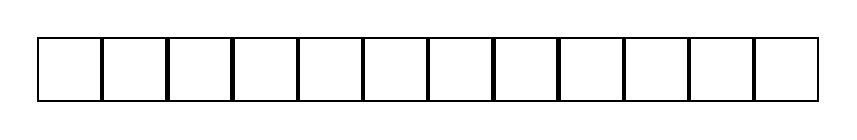
\begin{tikzpicture}
    [every node/.style={inner sep=4pt,draw,thick,minimum size=.8cm},%
    lineDecorate/.style={-,thick}]
%    \footnotesize
    \pgfmatrix{rectangle}{center}{}
    {\pgfusepath{}}{\pgfpointorigin}{\let\&=\pgfmatrixnextcell}
    {
      \node(0){}; \& \node(2){}; \& \node(3){}; \& \node(6){}; \&
      \node(4){}; \& \node(8){}; \& \node(10){}; \& \node(17){}; \&
      \node(13){}; \& \node(19){}; \& \node(24){}; \&
      \node(23){}; \\
    }
\end{tikzpicture}
}

\only<3->{
  \begin{center}
    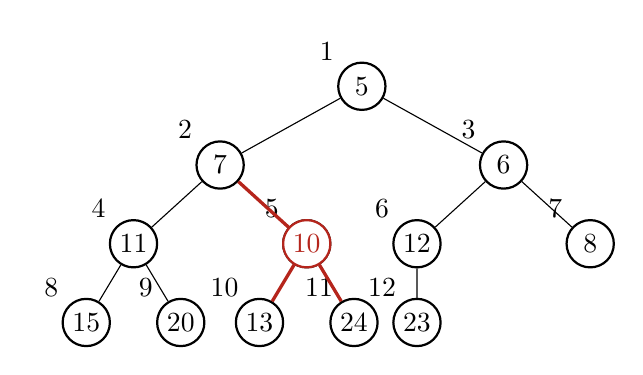
\begin{tikzpicture}[level distance=1cm,
      tnode/.style={circle,draw,minimum width=3pt,thick}]
      \tikzstyle{every node}=[circle,draw,minimum
      size=.6cm,thick,inner sep=1pt] \tikzstyle{level 1}=[sibling
      distance=36mm] \tikzstyle{level 2}=[sibling distance=22mm]
      \tikzstyle{level 3}=[sibling distance=12mm] \node[label=above
      left:\blue{1}] (Rac) {5} %L0
      child{ node[label=above left:\blue{2}] (P) {7} %L1
        child{ node[label=above left:\blue{4}] {11} child{
            node[label=above left:\blue{8}] {15}} child{
            node[label=above left:\blue{9}] {20}}} child{
          node[label=above left:\blue{5}] (V) {10} child{ node[label=above
            left:\blue{10}] (F1) {13}} child{ node[label=above
            left:\blue{11}] (F2) {24}}}} child{ node[label=above
        left:\blue{3}] (D1) {6} %L1
        child{ node[label=above left:\blue{6}] (D2) {12}
          child{node[label=above left:\blue{12}] {23}}} child{
          node[label=above left:\blue{7}] {8} }} ;
      \node[visible on=<4->,BrickRed,fill=white] at (V) {10};
      \path[very thick]
      (V) edge[visible on=<4->,BrickRed] (P)
          edge[visible on=<4->,BrickRed] (F1)
          edge[visible on=<4->,BrickRed] (F2);
    \end{tikzpicture}
  \end{center}

  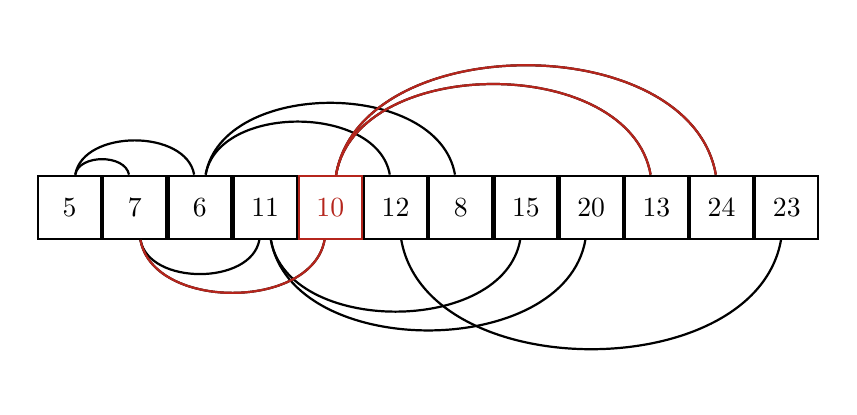
\begin{tikzpicture}
    [every node/.style={inner sep=4pt,draw,thick,minimum size=.8cm},%
    lineDecorate/.style={-,thick}]
%    \footnotesize
    \pgfmatrix{rectangle}{center}{}
    {\pgfusepath{}}{\pgfpointorigin}{\let\&=\pgfmatrixnextcell}
    {
      \node(0){$5$}; \& \node(2){$7$}; \& \node(3){$6$}; \& \node(6){$11$}; \&
      \node(4){$10$}; \& \node(8){$12$}; \& \node(10){$8$}; \& \node(17){$15$}; \&
      \node(13){$20$}; \& \node(19){$13$}; \& \node(24){$24$}; \&
      \node(23){$23$}; \\
    }
    \path
    \foreach \startNode/\endNode/\bend in {
      0/2/bend left, 0/3/bend left, 2/6/bend right, 2/4/bend right,
      3/8/bend left, 3/10/bend left, 6/17/bend right, 6/13/bend right,
      4/19/bend left, 4/24/bend left, 8/23/bend right}
    {
      (\startNode) edge[lineDecorate,\bend=80] (\endNode)
    };
    \node[BrickRed,visible on=<5->,fill=white] at (4) {10};
    \path 
    (4) edge[visible on=<5->,BrickRed,lineDecorate,bend left=80] (19)
    (4) edge[visible on=<5->,BrickRed,lineDecorate,bend left=80] (24)
    (2) edge[visible on=<5->,BrickRed,lineDecorate,bend right=80] (4);
\end{tikzpicture}
}
\end{frame}

\begin{frame}
  \frametitle{Tas et tableau}
  Soit \textbf{v} le n{\oe}ud à la position \red{i} du tableau ($v = T[i]$)
  \begin{itemize}
  \item \red{père}(\textbf{v}) $=$ \uncover<2->{$\red{\mathbf{T[\lfloor\frac{i}{2}\rfloor]}}$}
  \item \red{fils}(\textbf{v}) $=$ \uncover<3->{$\red{\mathbf{T[2i]}}$ et $\red{\mathbf{T[2i+1]}}$}
  \end{itemize}
\end{frame}



% ============================================
%============================================
\lecture{Arbres binaires de recherche}{lec-arbre-recherche}
%============================================
%============================================
\begin{frame}
  \frametitle{Arbre binaire de recherche}
 Arbre binaire dont les clés sont stockées de manière à satisfaire à la propriété d’arbre binaire de recherche :
Soit $x$ un n{\oe}ud d’un arbre binaire de recherche 
 \begin{itemize}
  \item Si y est un n{\oe}ud du \red{sous-arbre gauche} de x, alors la clé de $y$ est \red{$\mathbf{\leq}$} à la clé de $x$
 \item Si y est un n{\oe}ud du \red{sous-arbre droit} de x, alors la clé de $y$ est \red{$\mathbf{\geq}$} à la clé de $x$
  \end{itemize}
  \end{frame}

\begin{frame} \frametitle{Arbre binaire de recherche : représentation}
Chaque n{\oe}ud de l'arbre est un objet.\\ En plus du champ \red{\emph{clé}} (et des données satellites), chaque n{\oe}ud contient les champs \red{\emph{gauche}}, \red{\emph{droit}} et \red{\emph{pere}}
qui pointent sur le n{\oe}ud correspondant respectivement à son fils gauche, à son fils droit et à son père. 
\\ Si le père ou l'un des fils, est absent, le champ correspondant contient la valeur $NIL$. \\
La racine est le seul n{\oe}ud de l'arbre dont le champ \emph{pere} vaut $NIL$.
%\begin{itemize}
%\item estVide(T) retourne vrai si l’arbre T est vide
%\item val(T) retourne la clé de la racine d’un arbre T non vide
%\item filsgauche(T) et filsdroit(T) retournent respectivement la racine du sous-arbre gauche et du sous-arbre droit de l’arbre T.
%\end{itemize}
\end{frame}

\begin{frame}
\frametitle{Recherche d'un n{\oe}ud ayant une clé donnée}
Etant donné un pointeur sur la racine de l'arbre $x$ et une clé $k$ retourne un pointeur sur un n{\oe}ud ayant la clé donnée s'il en existe un; sinon retourne $NIL$.\\
   \begin{tabbing}
    aaa\=aaa\=aaa\kill
    \textbf{Rechercher}(x,k) \\
    \uncover<2->{\> \textbf{si} x=NIL ou clé(x)=k$\,$ \= \textbf{alors} \textsl{retourner} \textbf{x} \textbf{fin si} \\}
  \uncover<3->{\> \textbf{si} k$<$ clé(x) \\ \> \ \textbf{alors} \textsl{retourner} \textbf{Rechercher}(gauche(x),k) 
\\}
 \uncover<4->{\> \ \textbf{sinon} \textsl{retourner} \textbf{Rechercher}(droit(x),k)  \\
  \> \textbf{fin si}}
 \end{tabbing}
%  \uncover<5->{Complexité $= $}\uncover<6->{\red{$\mathbf{O(n)}$} où $\mathbf{n}$ est la longueur de la liste.}   
\end{frame}

\begin{frame}
  \frametitle{Minimum}
Retourne le n{\oe}ud ayant la clé minimale de l’arbre binaire de recherche enraciné au n{\oe}ud $x$
s'il en existe un; sinon retourne $NIL$ \\
\uncover<2->{   \begin{tabbing}
    aaa\=aaa\=aaa\kill
    \textbf{Minimum}(x) \\
    \textbf{tant que} gauche(x)$\neq NIL$ \textbf{faire} \\ \> $x\leftarrow gauche(x)$\\
  \textbf{fin tant que}\\
    % }
 \textsl{retourner} x \\
   \end{tabbing}}
%  \uncover<5->{Complexité $= $}\uncover<6->{\red{$\mathbf{O(n)}$} où $\mathbf{n}$ est la longueur de la liste.}   
\end{frame}

\begin{frame}
  \frametitle{Successeur d’un n{\oe}ud}
Considérer un arbre binaire de recherche ayant toutes les clés distinctes. Etant donné un n{\oe}ud $x$, retourner le successeur de $x$ s’il existe ou $NIL$ autrement. \\
Le \red{successeur d’un n{\oe}ud $x$ est le n{\oe}ud possédant la plus petite clé supérieure à la clé de $x$}. \\
\uncover<2->{
Deux cas :
\begin{enumerate}
\item \red{Le sous-arbre droit de l'arbre enraciné en $x$ n’est pas vide $\rightarrow$}} \uncover<3->{ le successeur de $x$ est le n{\oe}ud  le plus à gauche dans ce sous-arbre droit }
\uncover<4->{\item \red{Le sous-arbre droit de l'arbre enraciné en $x$ est vide et $x$ a un successeur $y$ $\rightarrow$} }  \uncover<5->{$y$ est le premier ancêtre de $x$ dont le fils de gauche est aussi un ancêtre de $x$}
\end{enumerate}

\end{frame}


\begin{frame}
\frametitle{Successeur d’un n{\oe}ud}
 \begin{tabbing}
   aaa\=aaa\=aaa\kill
 \textbf{Successeur}(x) \\
\textbf{si} droit(x) $\neq$ NIL \textbf{alors}\\  \> \textbf{retourner}  \textbf{Minimum}(droit(x))\\
$y \leftarrow pere(x)$ \\
\textbf{tant que} $y\neq NIL$ et $x=droit(y)$ \textsl{faire} \\
\>$x \leftarrow y$ \\
\> $y \leftarrow pere(y)$ \\
\textbf{fin tant que} \\
\textbf{retourner} y
\end{tabbing}
%%  \uncover<5->{Complexité $= $}\uncover<6->{\red{$\mathbf{O(h)}$} où $\mathbf{h}$ est la hateur de l'arbre de recherche.}   
\end{frame}


\begin{frame}
\frametitle{Insertion d’une nouvelle valeur dans un arbre binaire de recherche}
Pour insérer une nouvelle valeur $v$ dans un arbre binaire de recherche $T$, la procédure \textbf{Insérer} prend en entrée $T$ et un n{\oe}ud $z$ avec clé $v$ et ayant les champs \emph{gauche(z)}=NIL et \emph{droit(z)}=NIL.\\
\end{frame}

\begin{frame}
\frametitle{Insertion: pseudocode}
\begin{tabbing}
   aaa\=aaa\=aaa\kill
 \textbf{Insérer}(T,z) \\
\{$y \leftarrow NIL$\\
$x \leftarrow T$\\
\textbf{tant que} x $\neq$ NIL \textbf{faire} \\ 
\> $y \leftarrow x$ \\
\> \textbf{si} clé(z) $<$ clé(x) \\
\>\> \textbf{alors}  $x \leftarrow gauche(x)$ \\
\> \> \textbf{sinon} $x \leftarrow droit(x)$ \\
\textbf{fin tant que} \\
$pere(z) \leftarrow y$\\
\textbf{si} y =NIL \textbf{alors} $T \leftarrow z$ \hfill $~~~~~~~~~~~~~~~$\texttt{/* arbre T était vide */}\\
\textbf{sinon si} clé(z)$<$clé(y) \\ \> \> \textbf{alors} $gauche(y) \leftarrow z$\\
\> \> \textbf{sinon} $droit(y) \leftarrow z$\\ \} 
\end{tabbing}
%%  \uncover<5->{Complexité $= $}\uncover<6->{\red{$\mathbf{O(h)}$} où $\mathbf{h}$ est la hateur de l'arbre de recherche.}   
\end{frame}



\begin{frame}
\frametitle{Suppression d’un n{\oe}ud dans un arbre binaire de recherche}
La procédure pour supprimer un n{\oe}ud  $z$ donné dans un arbre binaire de recherche $T$, prend en entrée un pointeur sur $z$.\\
Trois cas possibles :
\begin{itemize}
\item \red{$z$ n'a pas de fils} $\rightarrow$ on modifie le père de $z$ pour remplacer $z$ par NIL dans le champ fils correspondant.
\item \red{$z$ a un seul fils} $\rightarrow$ on "détache" $z$ en créant un nouveau lien entre le père de $z$ et le fils de $z$.
\item \red{$z$ a deux fils} $\rightarrow$ on "détache" le successeur de $z$, $y$, qui n'a pas de fils gauche et on remplace la clé de $z$ par la clé de $y$.
\end{itemize}
\end{frame}



\begin{frame}\frametitle{Suppression d’un n{\oe}ud}
\begin{tabbing}
   aaa\=aaa\=aaa\kill
 \textbf{Supprimer}(T,z) \\
\{\textbf{si} gauche(z)=NIL ou droit(z)=NIL \\ 
 \> \textbf{alors}  $y \leftarrow z$ \\
 \> \textbf{sinon}  y $\leftarrow$ \textbf{Successeur(z)} \textbf{fin si}\\
\ \textbf{si} gauche(y) $\neq$ NIL \\
\ \> \textbf{alors}  $x \leftarrow gauche(y)$ \\
\ \> \textbf{sinon}  $x \leftarrow droit(y)$ \textbf{fin si}\\
\ \textbf{si} x $\neq$ NIL  \\
\ \>\textbf{alors}  $pere(x) \leftarrow pere(y)$ \textbf{fin si}\\
\ \textbf{si} $pere(y)= NIL$ \\
\ \> \textbf{alors} $T \leftarrow x$ \\
\ \> \textbf{sinon si} y=gauche(pere(y))\\
\ \>\> \textbf{alors}  $gauche(pere(y)) \leftarrow x$ \\
\ \>\> \textbf{sinon}  $droit(pere(y)) \leftarrow x$ \textbf{fin si}\\
\ \textbf{si} $y \neq z$ \textbf{alors} clé(z) $\leftarrow$ clé(y) \textbf{fin si}\\
%\ \textbf{retourner} $y$
\}
\end{tabbing}
%%%  \uncover<5->{Complexité $= $}\uncover<6->{\red{$\mathbf{O(h)}$} où $\mathbf{h}$ est la hateur de l'arbre de recherche.}   
\end{frame}
\begin{frame}\frametitle{Complexité}
On peut  exécuter les opérations d'ensemble dynamique \textbf{Rechercher, Minimum, Maximum, Successeur, Insérer} et \textbf{Supprimer} en temps O(h) sur un arbre binaire de recherche de hauteur $h$.
\end{frame}

\end{document}
%%% Local Variables: 
%%% mode: latex
%%% TeX-master: t
%%% End: 
